\casesection{Upstream bedload sediment boundary condition (bcm)}
\label{case:e22-f22-c21}

\paragraph*{Purpose}
The purpose of these tests is to assess model behaviour for different options of upstream sediment boundary conditions that are available in Delft3D-FM. Following are the options for boundary conditions, which can be imposed at upstream open boundary: 

(i) 'bed level fixed', default or can be specified in morphological input file (no need to have boundary condition file)

(ii) 'depth', which implies specifying constant or varying bed level change in *.bcm file 

(iii) 'depth change', which implies constant or time varying rate of bed level change (i.e. bed level acceleration) in $*.bcm$ file, and 

(iv) 'transport including pores', which implies sediment transport rate including pores in *.bcm file. 
The test case number is e02-f22-c21.
\paragraph*{Linked claims}
Claims that are related to the test case are:
\begin{itemize}
\item The imposed upstream sediment transport conditions work in a proper way 
\end{itemize}
\begin{itemize}
	\item The results are consistent and comparable
\end{itemize}

\paragraph*{Approach}
A simple model is used to test the model behaviour for different options of upstream boundary condition for both Delft3D and Delft3D-FM. Four options are considered as mentioned above. Firstly, basic model behaviour is checked by imposing the conditions for 'Depth' and 'Depth change' such that there is no bed change at the boundary, and also zero transport for 'transport incl pores' option. Additional simulations are made by imposing certain values for these options to assess whether the changes at the boundary are consistent.     

Some tests are made with multiple sediment fractions (two in current tests) under similar condition as for single fraction. Besides, some additional tests are made under inclined bed (in transverse direction) condition to assess the model results for somewhat complex condition.    

\paragraph*{Model description}
A simple model of 16 m long, 1.6 m wide with a flat bed at a constant level of -0.5 is used. A discharge of 2000 l/s is imposed.  At the downstream boundary a water level of 0.17 m is imposed. A Ch\'ezy coefficient of 60 m$^0.5$/s is used for the channel roughness.   

\paragraph*{Results}
The comparison between bed levels and water levels simulated by Delft3D and Delft3D-FM after 20 minutes for fixed bed level condition is shown in Figure \ref{fig:e02-fxx-cxx:bedlevelstr0} and Figure \ref{fig:e02-fxx-cxx:waterlevelstr0} respectively. For the conditions with unchanged 'depth' (i.e. kept at level of -0.5), zero 'depth change' and zero 'transport', the results are depicted in Figure \ref{fig:e02-fxx-cxx:bedlevelstr001}, Figure \ref{fig:e02-fxx-cxx:waterlevelstr001}, Figure \ref{fig:e02-fxx-cxx:bedlevelstr002}, Figure \ref{fig:e02-fxx-cxx:waterlevelstr002}, Figure \ref{fig:e02-fxx-cxx:bedlevelstr003} and Figure \ref{fig:e02-fxx-cxx:waterlevelstr003} respectively.   

Similarly, the comparisons for other imposed conditions, namely 'Depth' (changing from -0.5 to -1.0 in 20 min of simulation time), 'Depth change' (from 0 to -0.5 m in 20 min of simulation time) and 'transport incl pores' (0.0002 m$^2$/s) are depicted in Figure \ref{fig:e02-fxx-cxx:bedlevelstr2}, Figure \ref{fig:e02-fxx-cxx:waterlevelstr2}, Figure \ref{fig:e02-fxx-cxx:bedlevelstr3}, Figure \ref{fig:e02-fxx-cxx:waterlevelstr3}, Figure \ref{fig:e02-fxx-cxx:waterlevelstr4} and Figure \ref{fig:e02-fxx-cxx:bedlevelstr4} respectively. 

For computations with multiple fractions, two similar fractions are used for the sake of simplicity. Several options with boundary condition 'transport incl pores' is tested to ensure correctness based on output results. Four scenarios of sediment boundary condition are tested and compared, namely (i) imposing same amount (0.0002 m$^2$/s) for both fractions, (ii) imposing 0.0002 m$^2$/s for fraction 1 and 0 m$^2$/s for fraction 2, (iii) imposing 0 m$^2$/s for fraction 1 and 0.0002 m$^2$/s, and (iv) imposing 0.0001 m$^2$/s for both fractions. 

The results for all four scenarios are depicted in Figure \ref{fig:e02-fxx-cxx:bedlevelstr5}, Figure \ref{fig:e02-fxx-cxx:waterlevelstr5}, Figure \ref{fig:e02-fxx-cxx:bedlevelstr6}, Figure \ref{fig:e02-fxx-cxx:waterlevelstr6}, Figure \ref{fig:e02-fxx-cxx:waterlevelstr7}, Figure \ref{fig:e02-fxx-cxx:bedlevelstr7}, Figure \ref{fig:e02-fxx-cxx:waterlevelstr8} and Figure \ref{fig:e02-fxx-cxx:bedlevelstr8} respectively.  

Results show consistency, for example result for first scenario shows decrease of erosion by half (comparing to uniform case) due to similar diameter and amount of additional sediment fraction imposed at the boundary (this can be assessed by comparing Figure \ref{fig:e02-fxx-cxx:bedlevelstr5} and Figure \ref{fig:e02-fxx-cxx:bedlevelstr4}). Also, results for second and third scenarios are consistent with the result of uniform case, since one of the fractions is 0 in these computations (this can be assessed by comparing Figure \ref{fig:e02-fxx-cxx:bedlevelstr6} and Figure \ref{fig:e02-fxx-cxx:bedlevelstr4}).

Results for some computational tests for inclined bed condition (in transverse direction) are depicted in Figure \ref{fig:e02-fxx-cxx:bedlevelstr9}, Figure \ref{fig:e02-fxx-cxx:waterlevelstr9}, Figure \ref{fig:e02-fxx-cxx:bedlevelstr10}, Figure \ref{fig:e02-fxx-cxx:waterlevelstr10}, Figure \ref{fig:e02-fxx-cxx:waterlevelstr11}, Figure \ref{fig:e02-fxx-cxx:bedlevelstr11}, Figure \ref{fig:e02-fxx-cxx:waterlevelstr12} and Figure \ref{fig:e02-fxx-cxx:bedlevelstr12}. 

There are some discrepancies for the computational scenarios with inclined channel bed.  Although this is expected given the fact that inclined bed causes transverse gradients. Imposing uniform sediment (or bed change) condition along the inclined boundary appears to be leading to some discrepancies and issues. This is evident even for fixed bed condition (as depicted in Figure \ref{fig:e02-fxx-cxx:bedlevelstr9}), so this issue cannot be fully attributed to the morphological boundary condition only. 
    

\paragraph*{Conclusion}

The computational results for different options and scenarios indicate the consistency in model behaviour, which implies that imposed sediment (bed) boundary conditions do work properly. Besides, most results of Delft3D FM resemble the result of Delft3D except for the condition 'depth change' (from 0 to -0.5 m) as shown in Figure \ref{fig:e02-fxx-cxx:bedlevelstr3}. As it can be seen from this figure, Delft3D shows larger erosion than imposed value (i.e. more than 1 m), while Delft3D-FM shows erosion of about 0.5 m, which is consistent with imposed condition. For the imposed boundary condition, which corresponds to unchanged bed level, the results are consistent for both models (as inferred from Figure \ref{fig:e02-fxx-cxx:bedlevelstr002}). This implies that the 'depth change' condition seems to induce some additional erosion in Delft3D model. This has to be explored further. 

There are some discrepancies for the computational scenarios with inclined channel bed. Although this is expected given the fact that inclined bed causes transverse gradients. Imposing uniform sediment (or bed change) condition along the inclined boundary appears to be leading to some discrepancies and issues. This is evident even for fixed bed condition, so this issue cannot be fully attributed to the morphological boundary condition only.

\pagebreak

\begin{figure}[htb]
	\begin{center}
		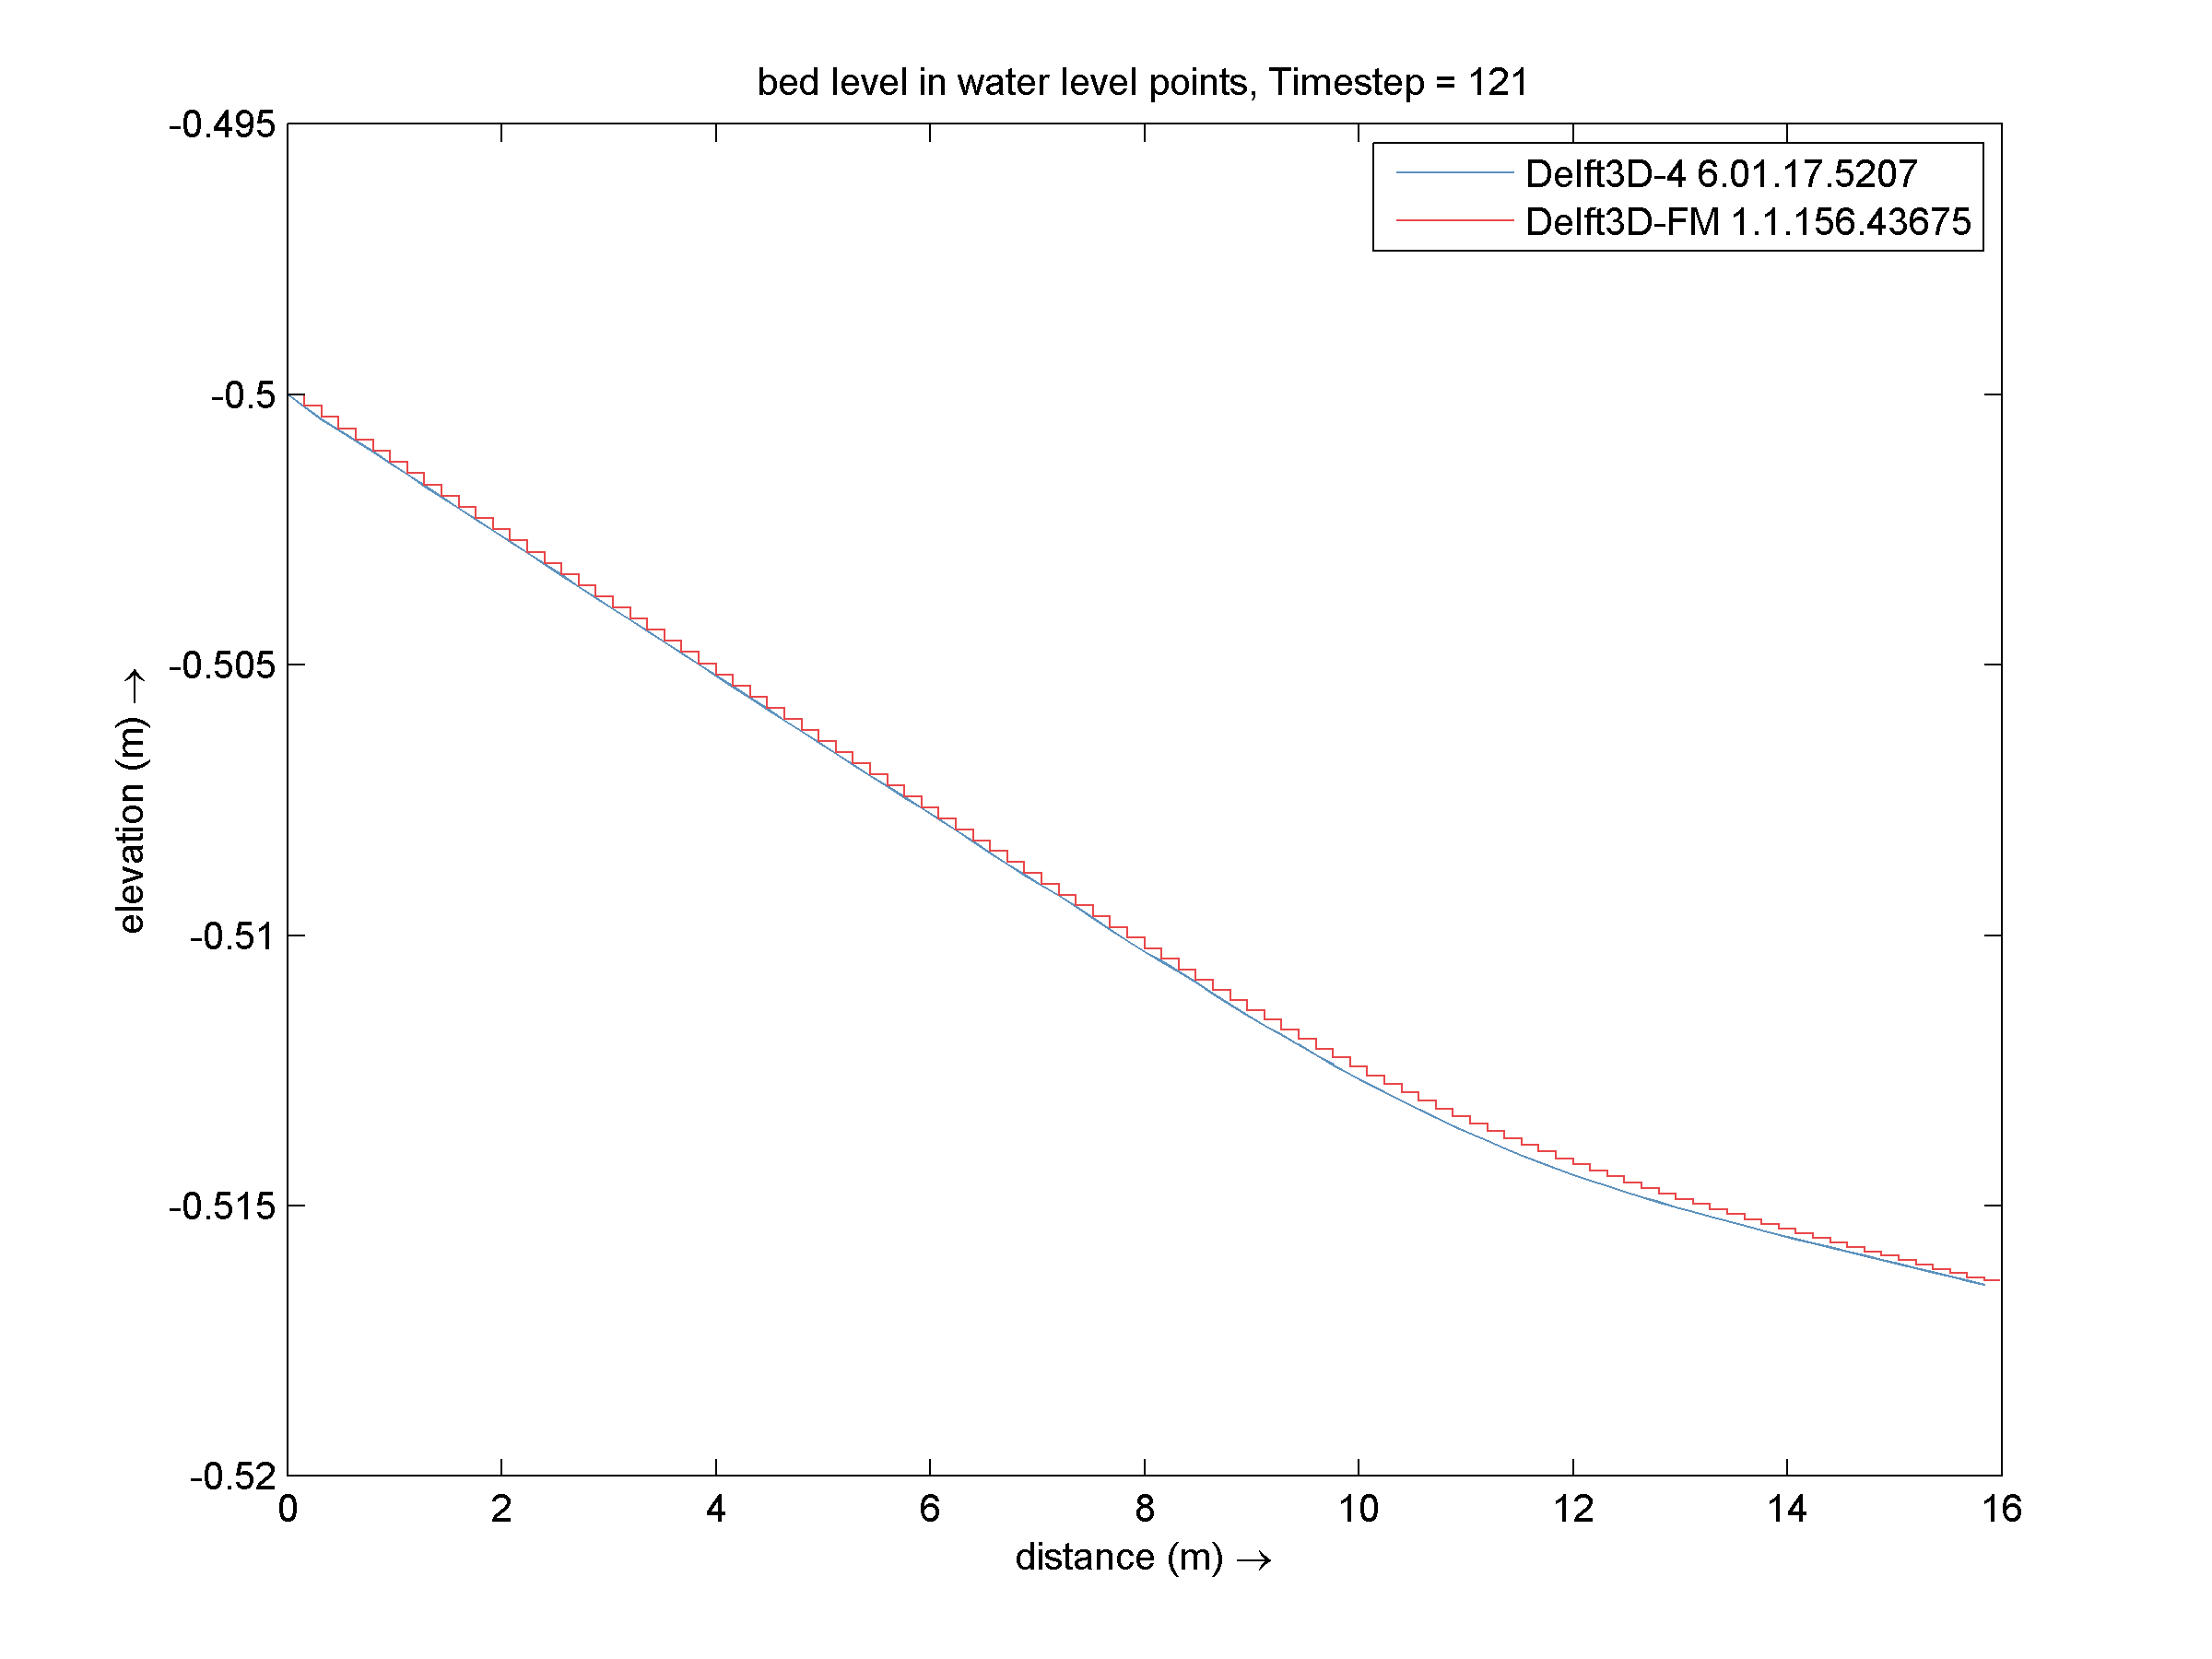
\includegraphics[width=0.70\textwidth]{figures/comparison_d3d_fm_blstr0.png}
	\end{center}
	\caption{Comparison of bed levels (fixed bed boundary condition).}\label{fig:e02-fxx-cxx:bedlevelstr0}
\end{figure}

\begin{figure}[htb]
	\begin{center}
		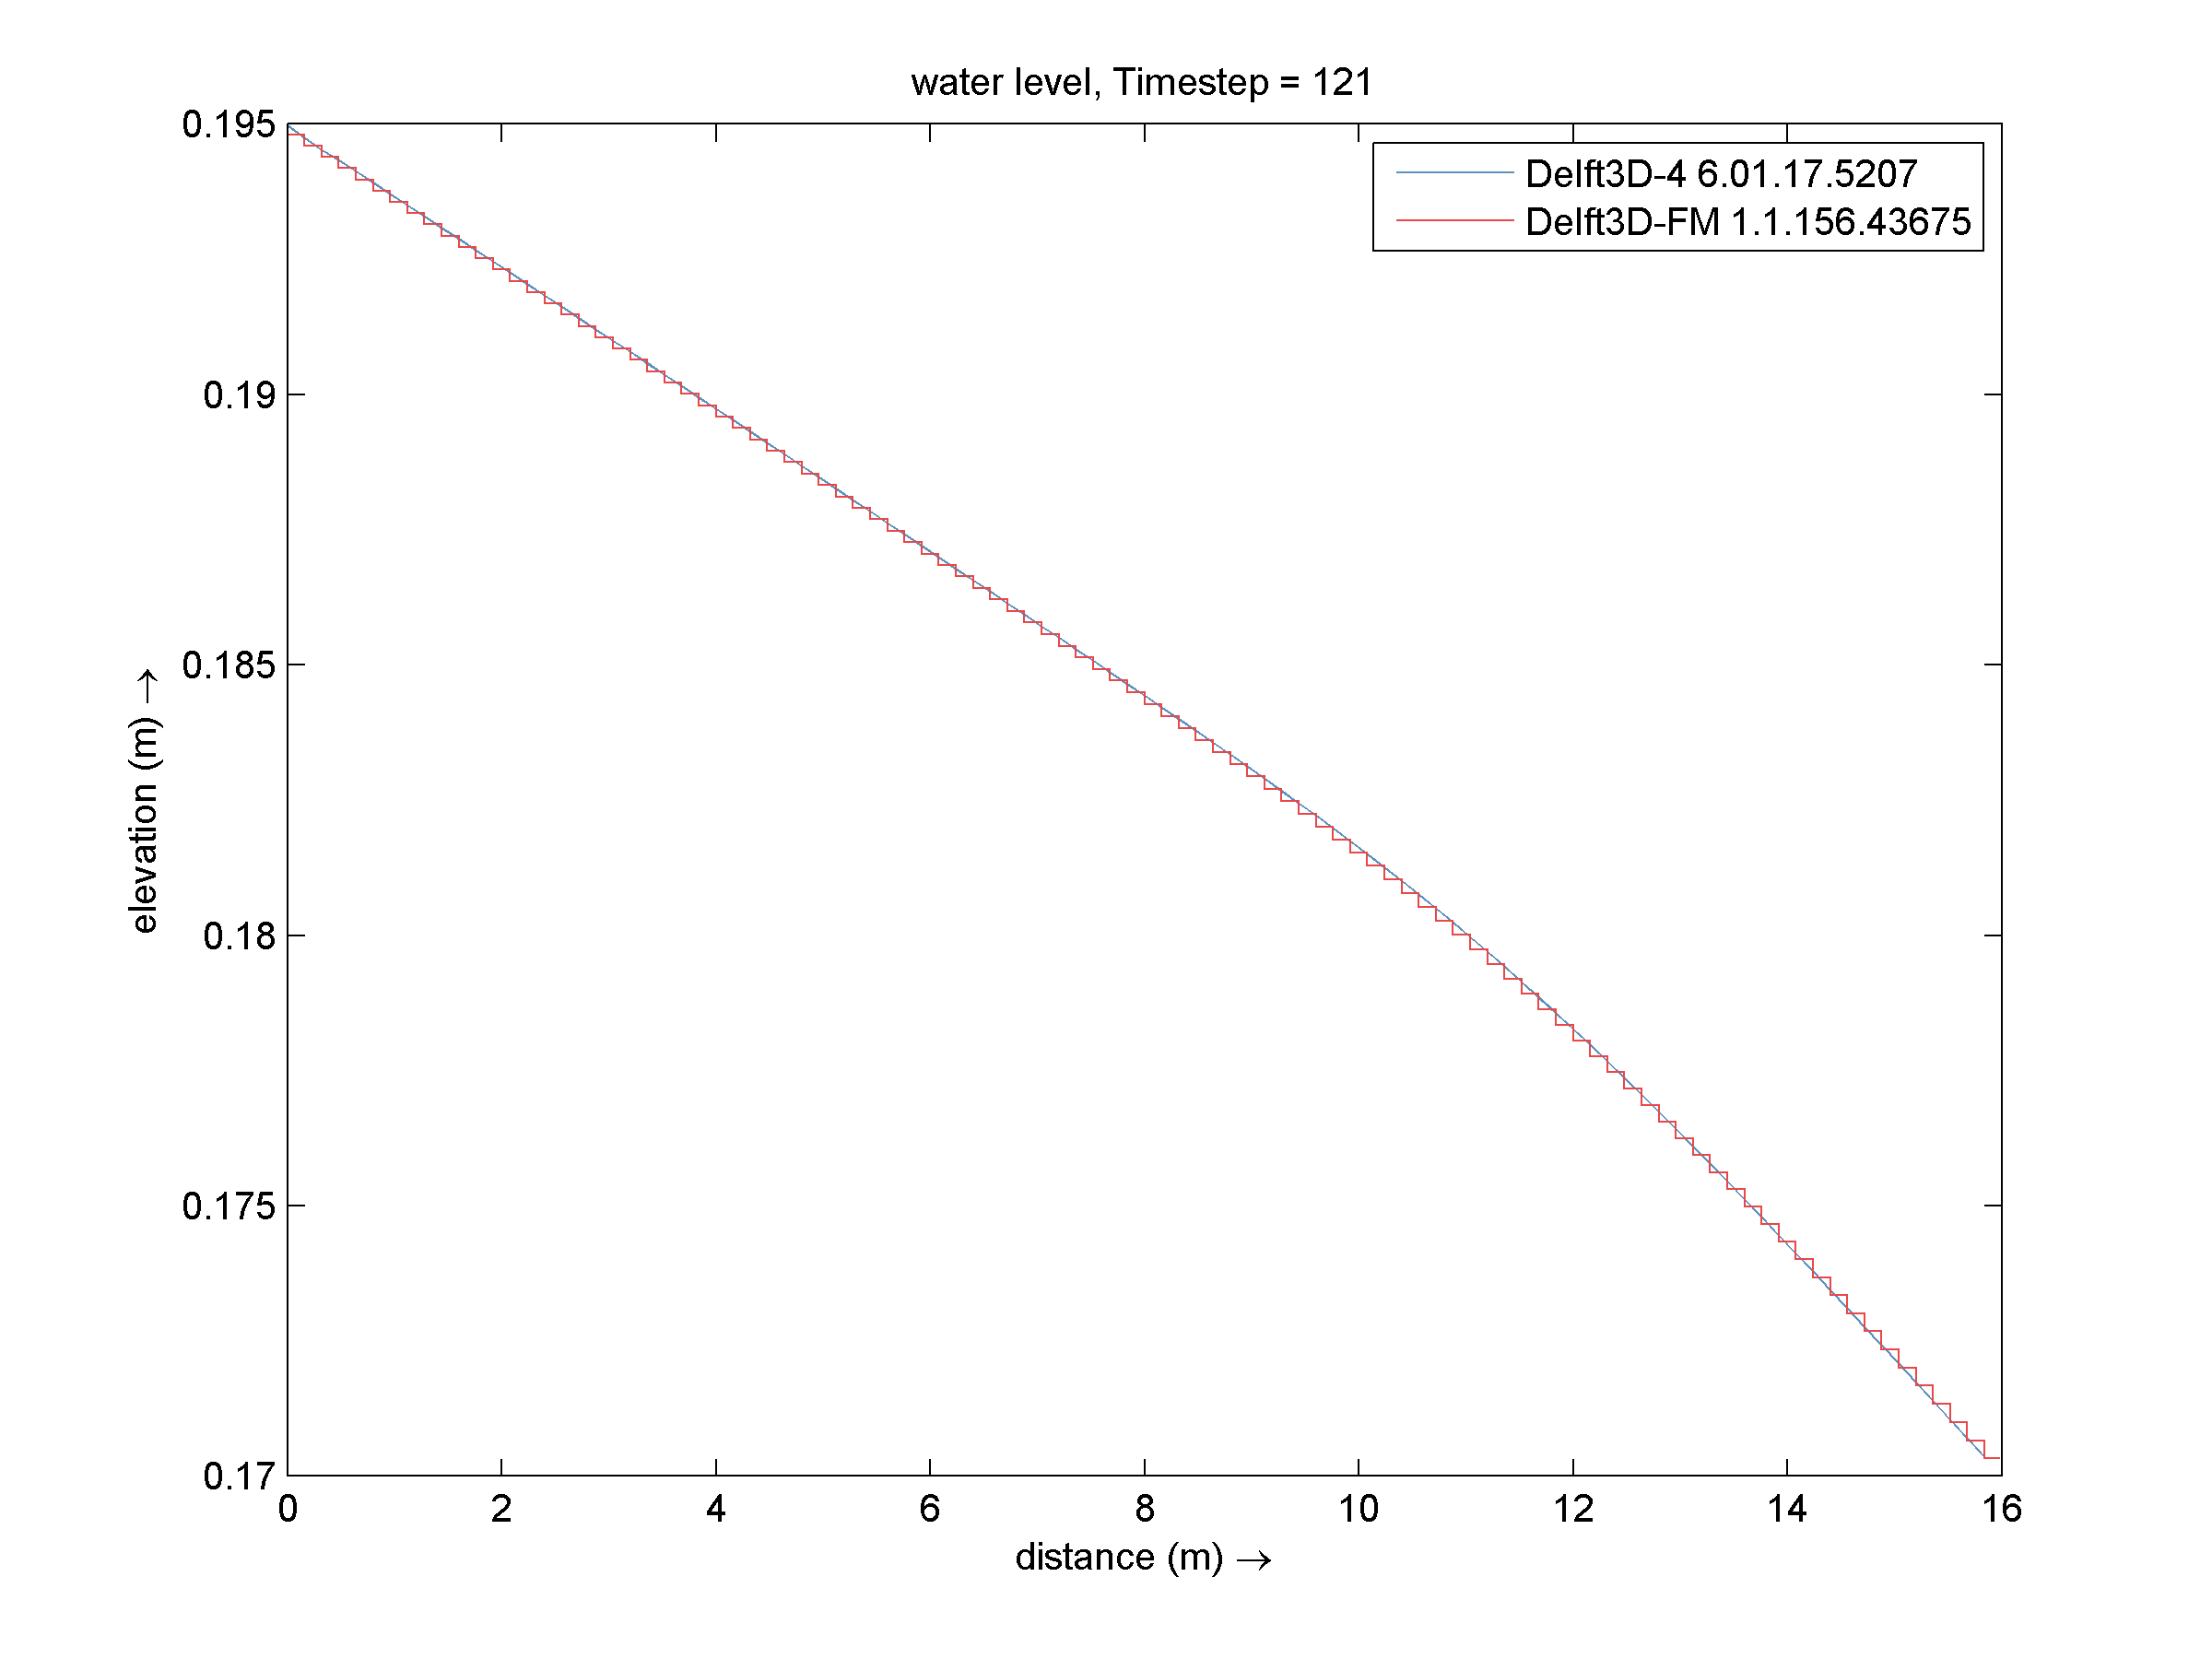
\includegraphics[width=0.70\textwidth]{figures/comparison_d3d_fm_wlstr0.png}
	\end{center}
	\caption{Comparison of water levels (fixed bed boundary condition).}\label{fig:e02-fxx-cxx:waterlevelstr0}
\end{figure}

\begin{figure}[htb]
	\begin{center}
		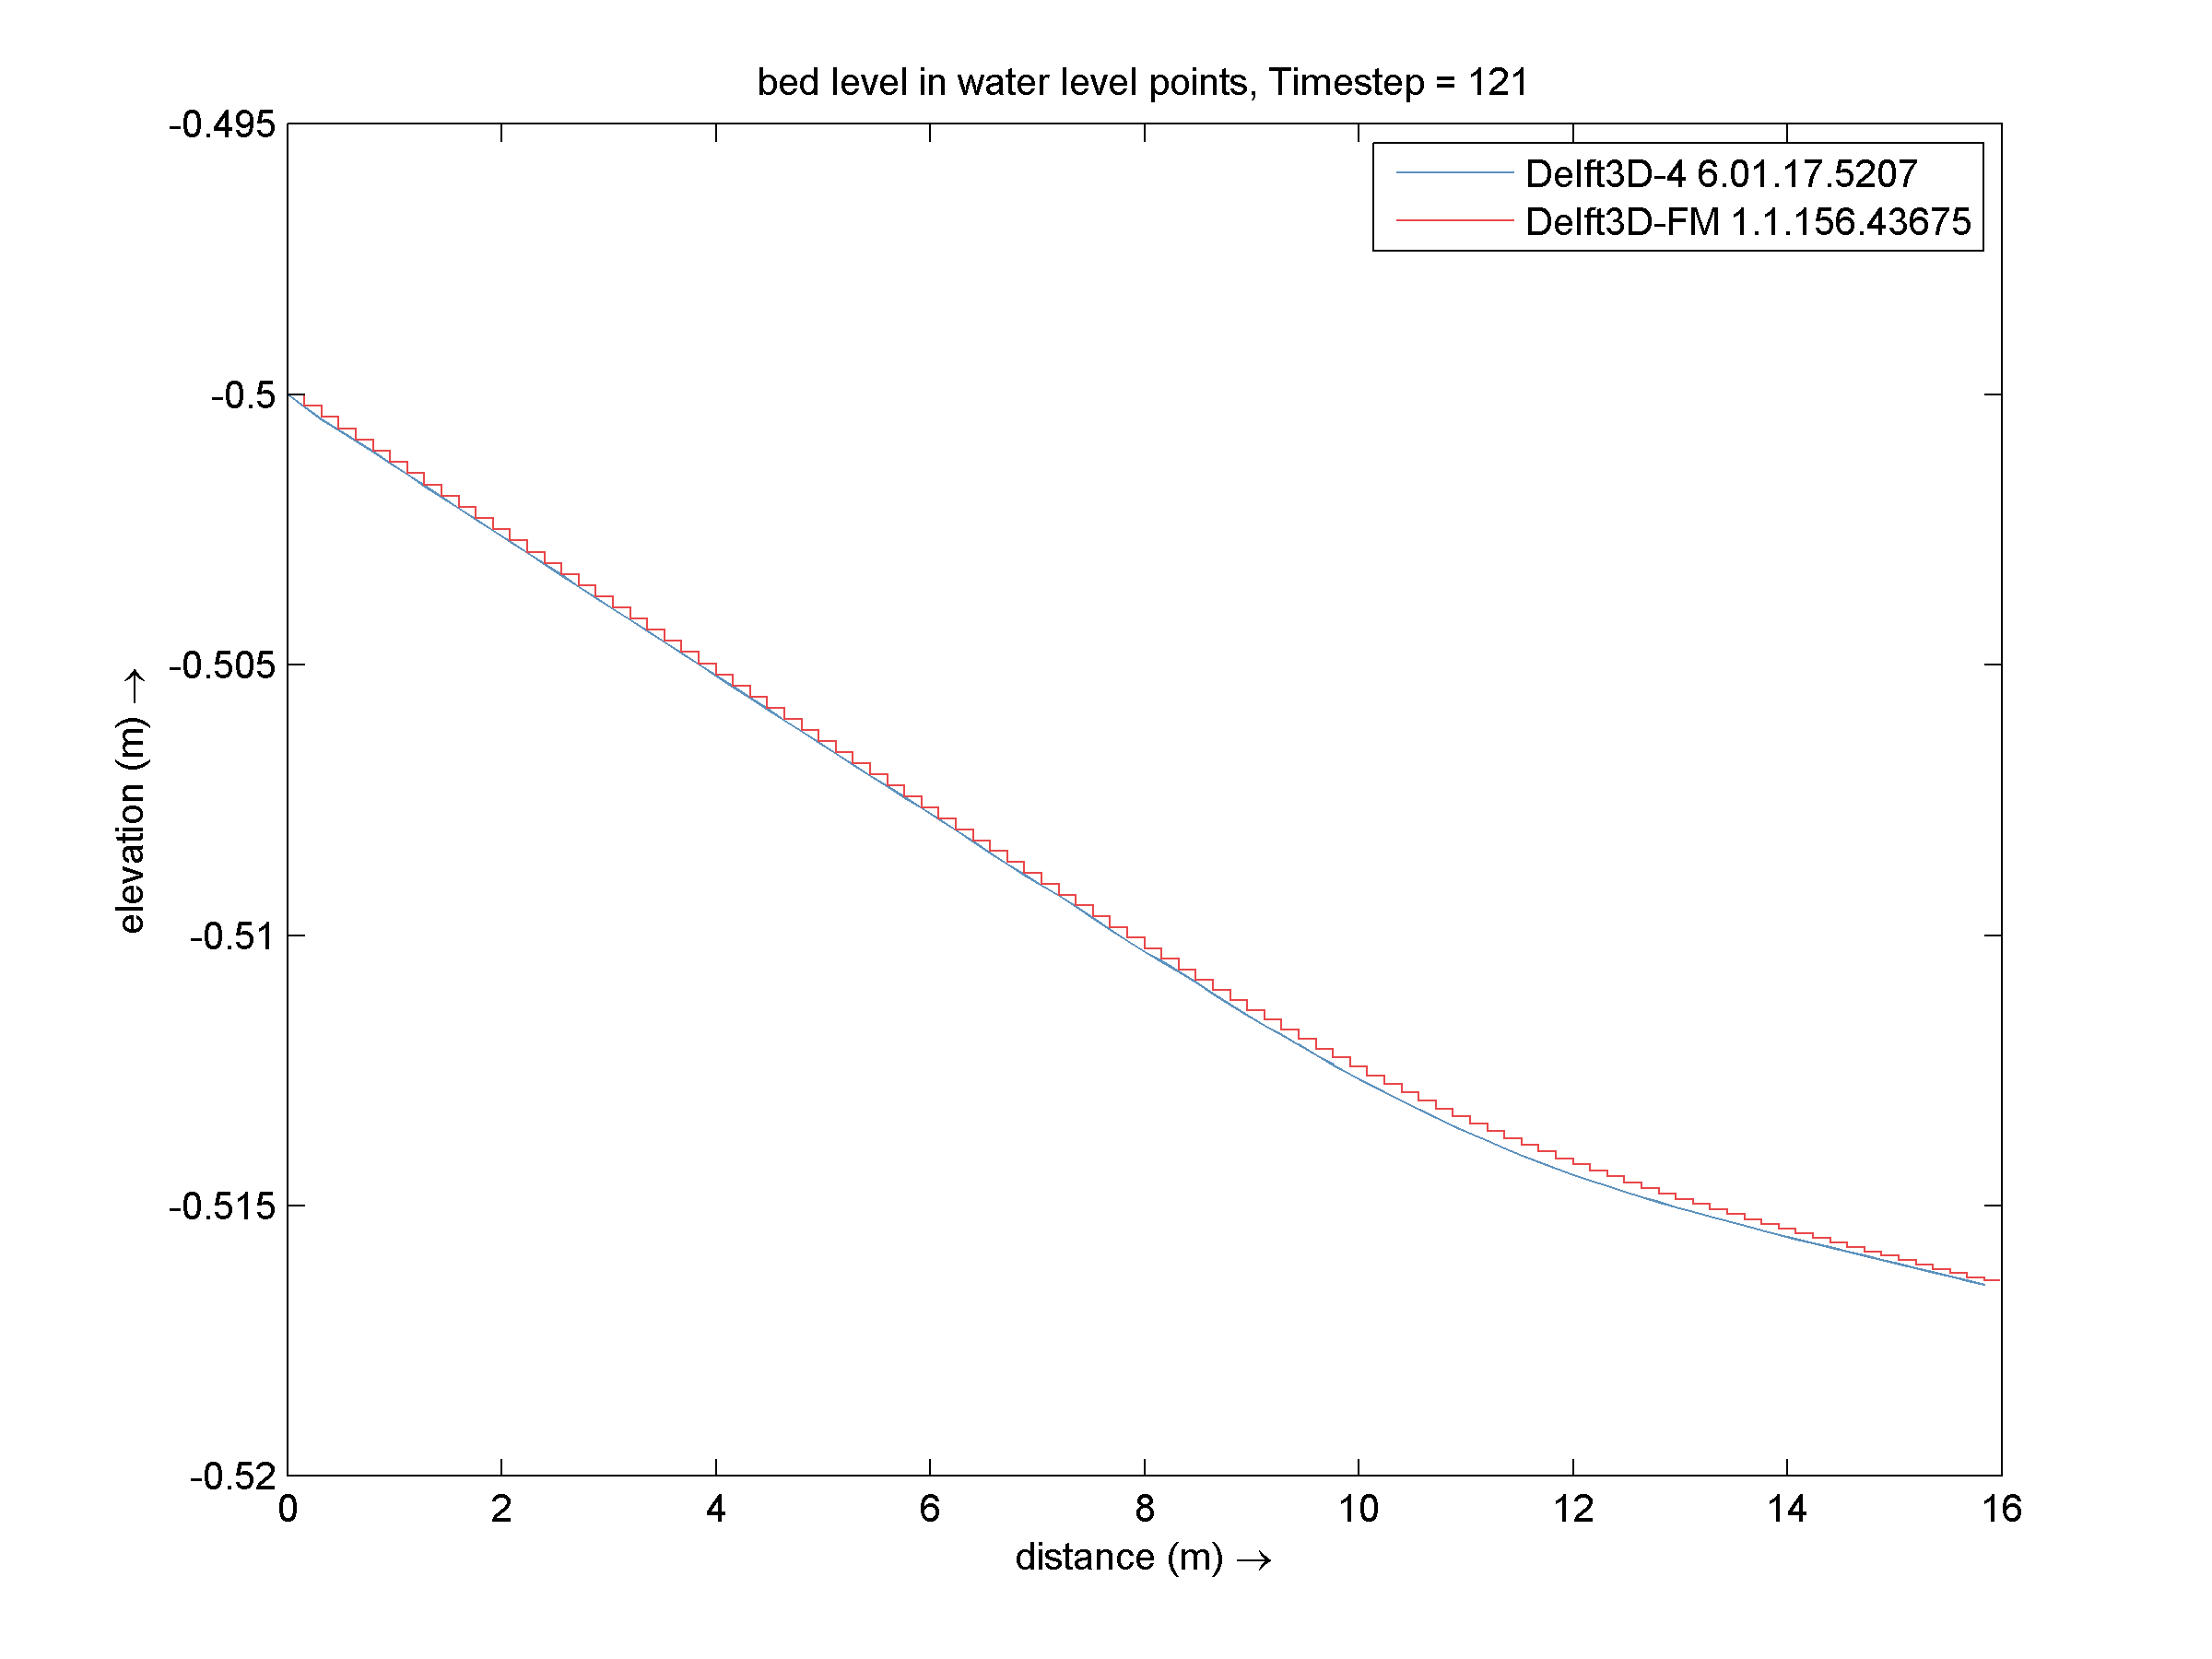
\includegraphics[width=0.70\textwidth]{figures/comparison_d3d_fm_blstr001.png}
	\end{center}
	\caption{Comparison of bed levels ('depth' = -0.5 m).}\label{fig:e02-fxx-cxx:bedlevelstr001}
\end{figure}

\begin{figure}[htb]
	\begin{center}
		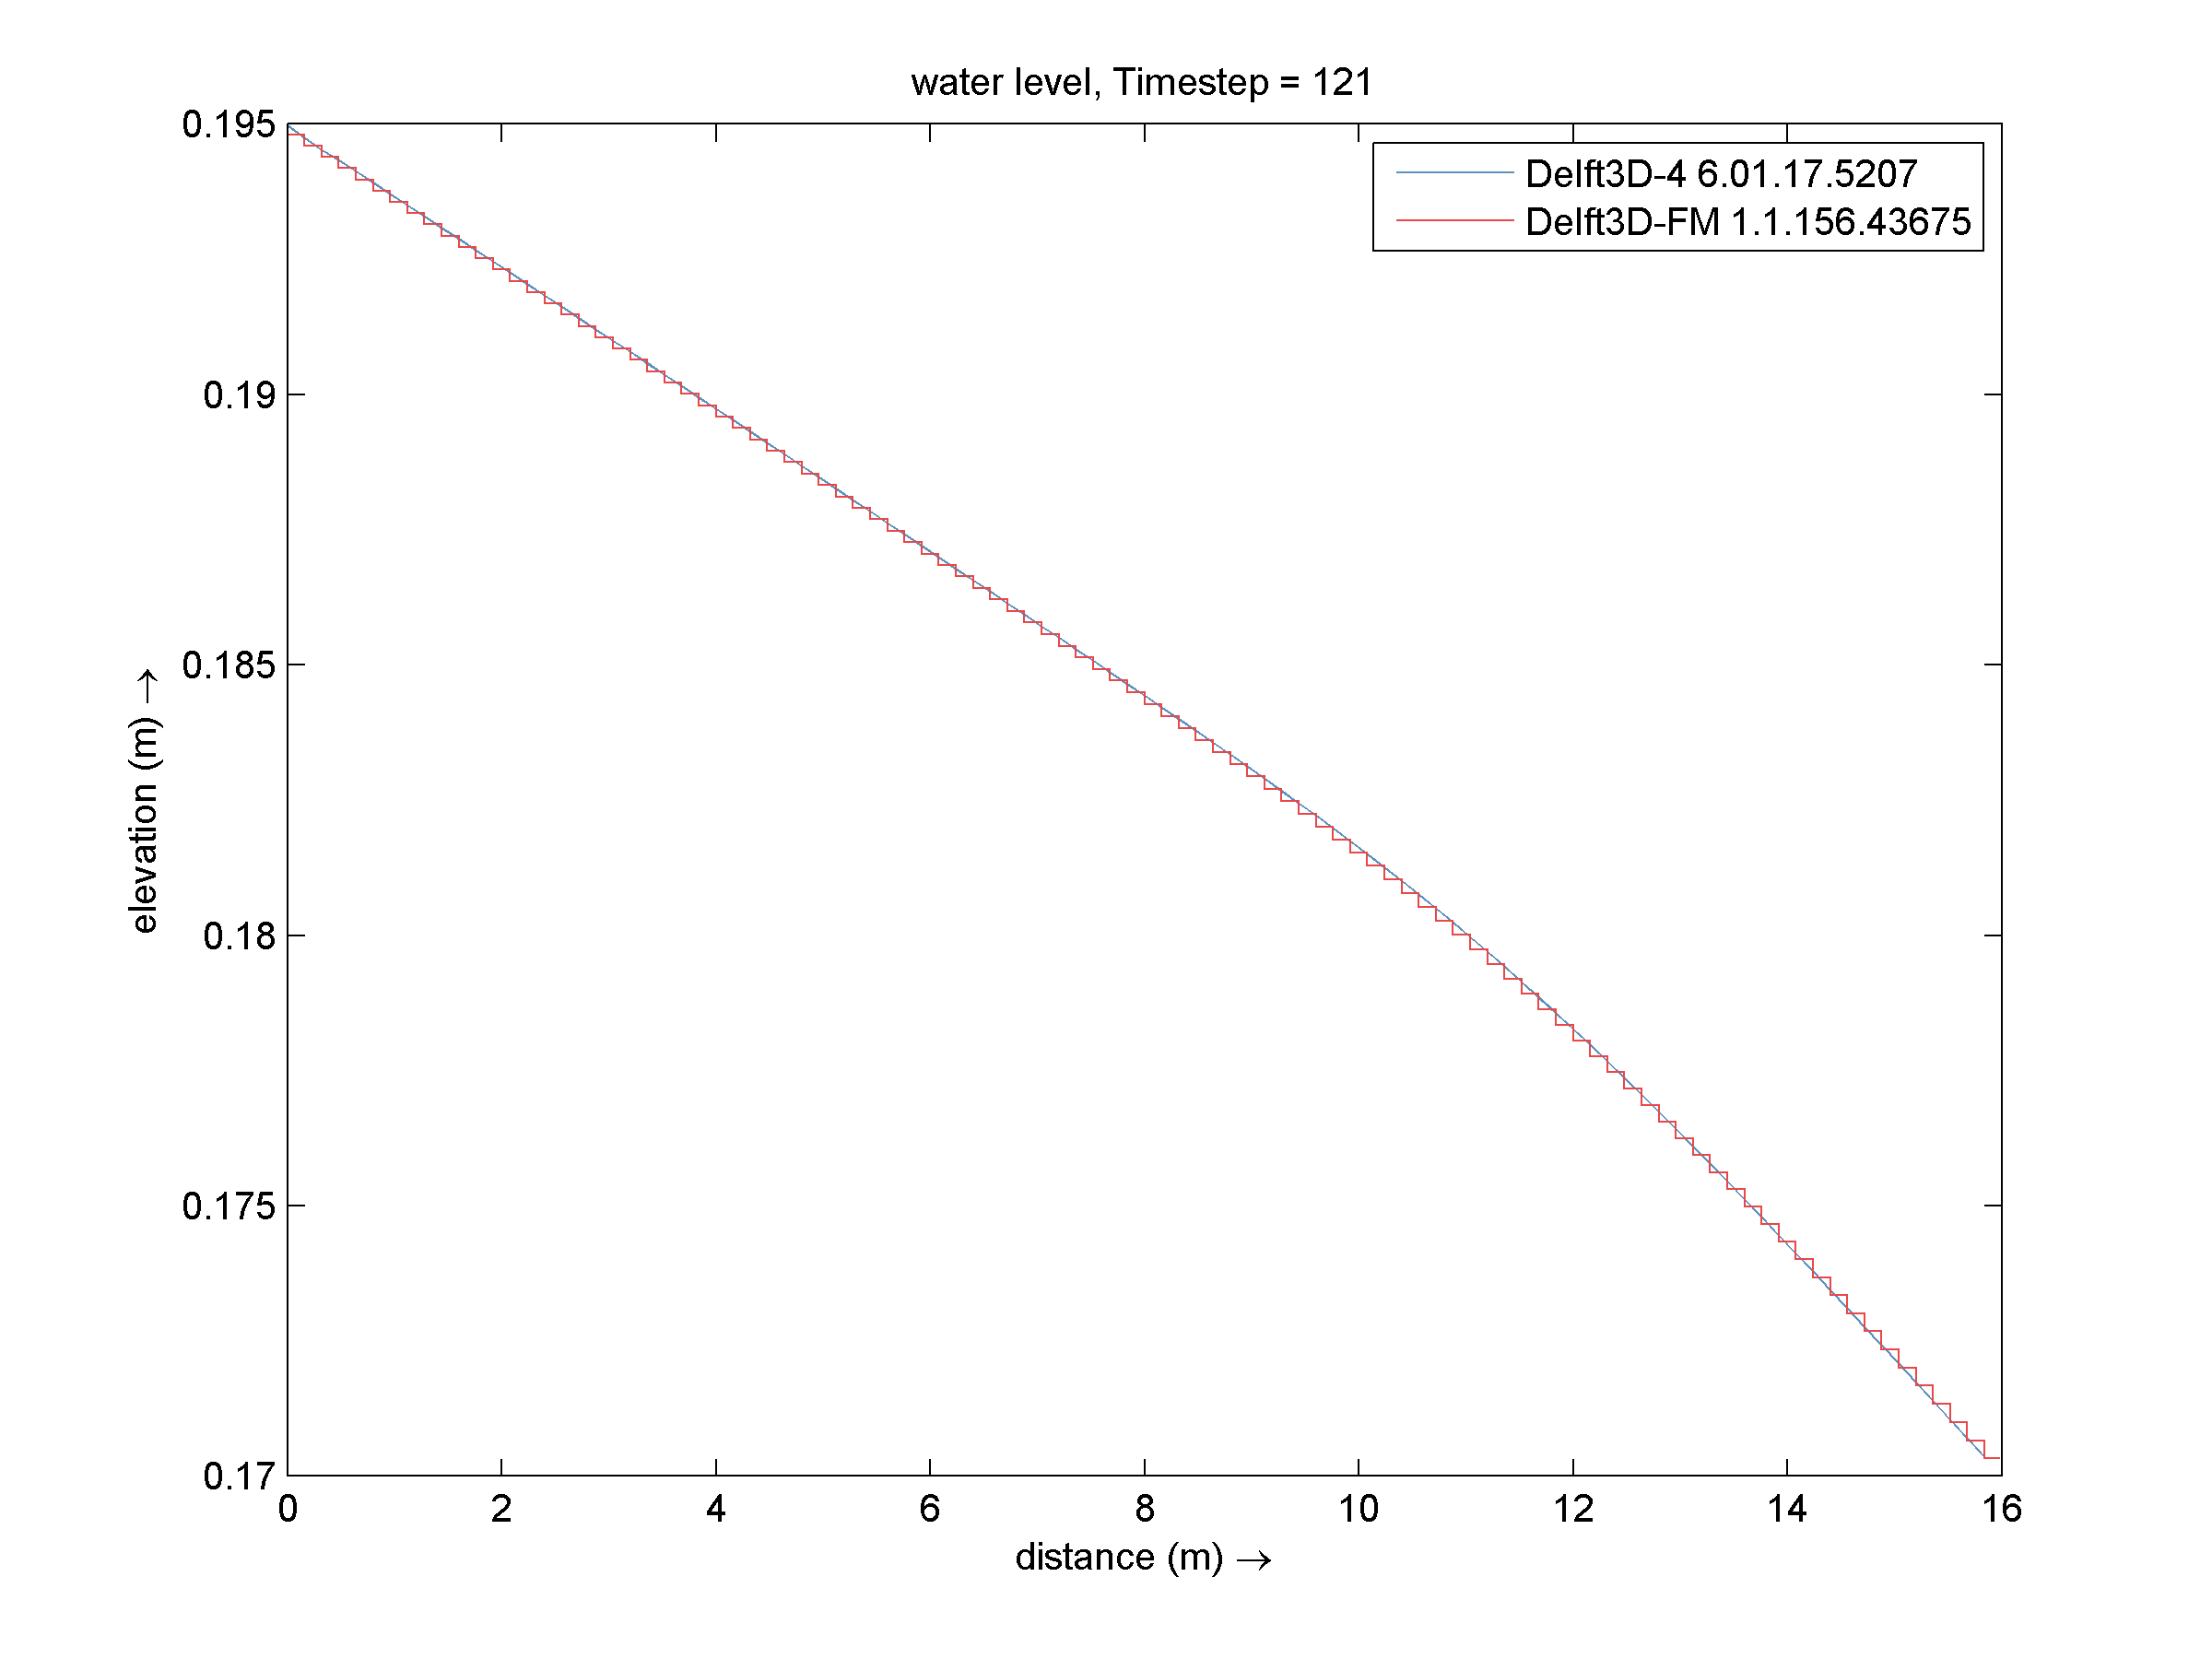
\includegraphics[width=0.70\textwidth]{figures/comparison_d3d_fm_wlstr001.png}
	\end{center}
	\caption{Comparison of water levels ('depth' = -0.5 m).}\label{fig:e02-fxx-cxx:waterlevelstr001}
\end{figure}

\begin{figure}[htb]
	\begin{center}
		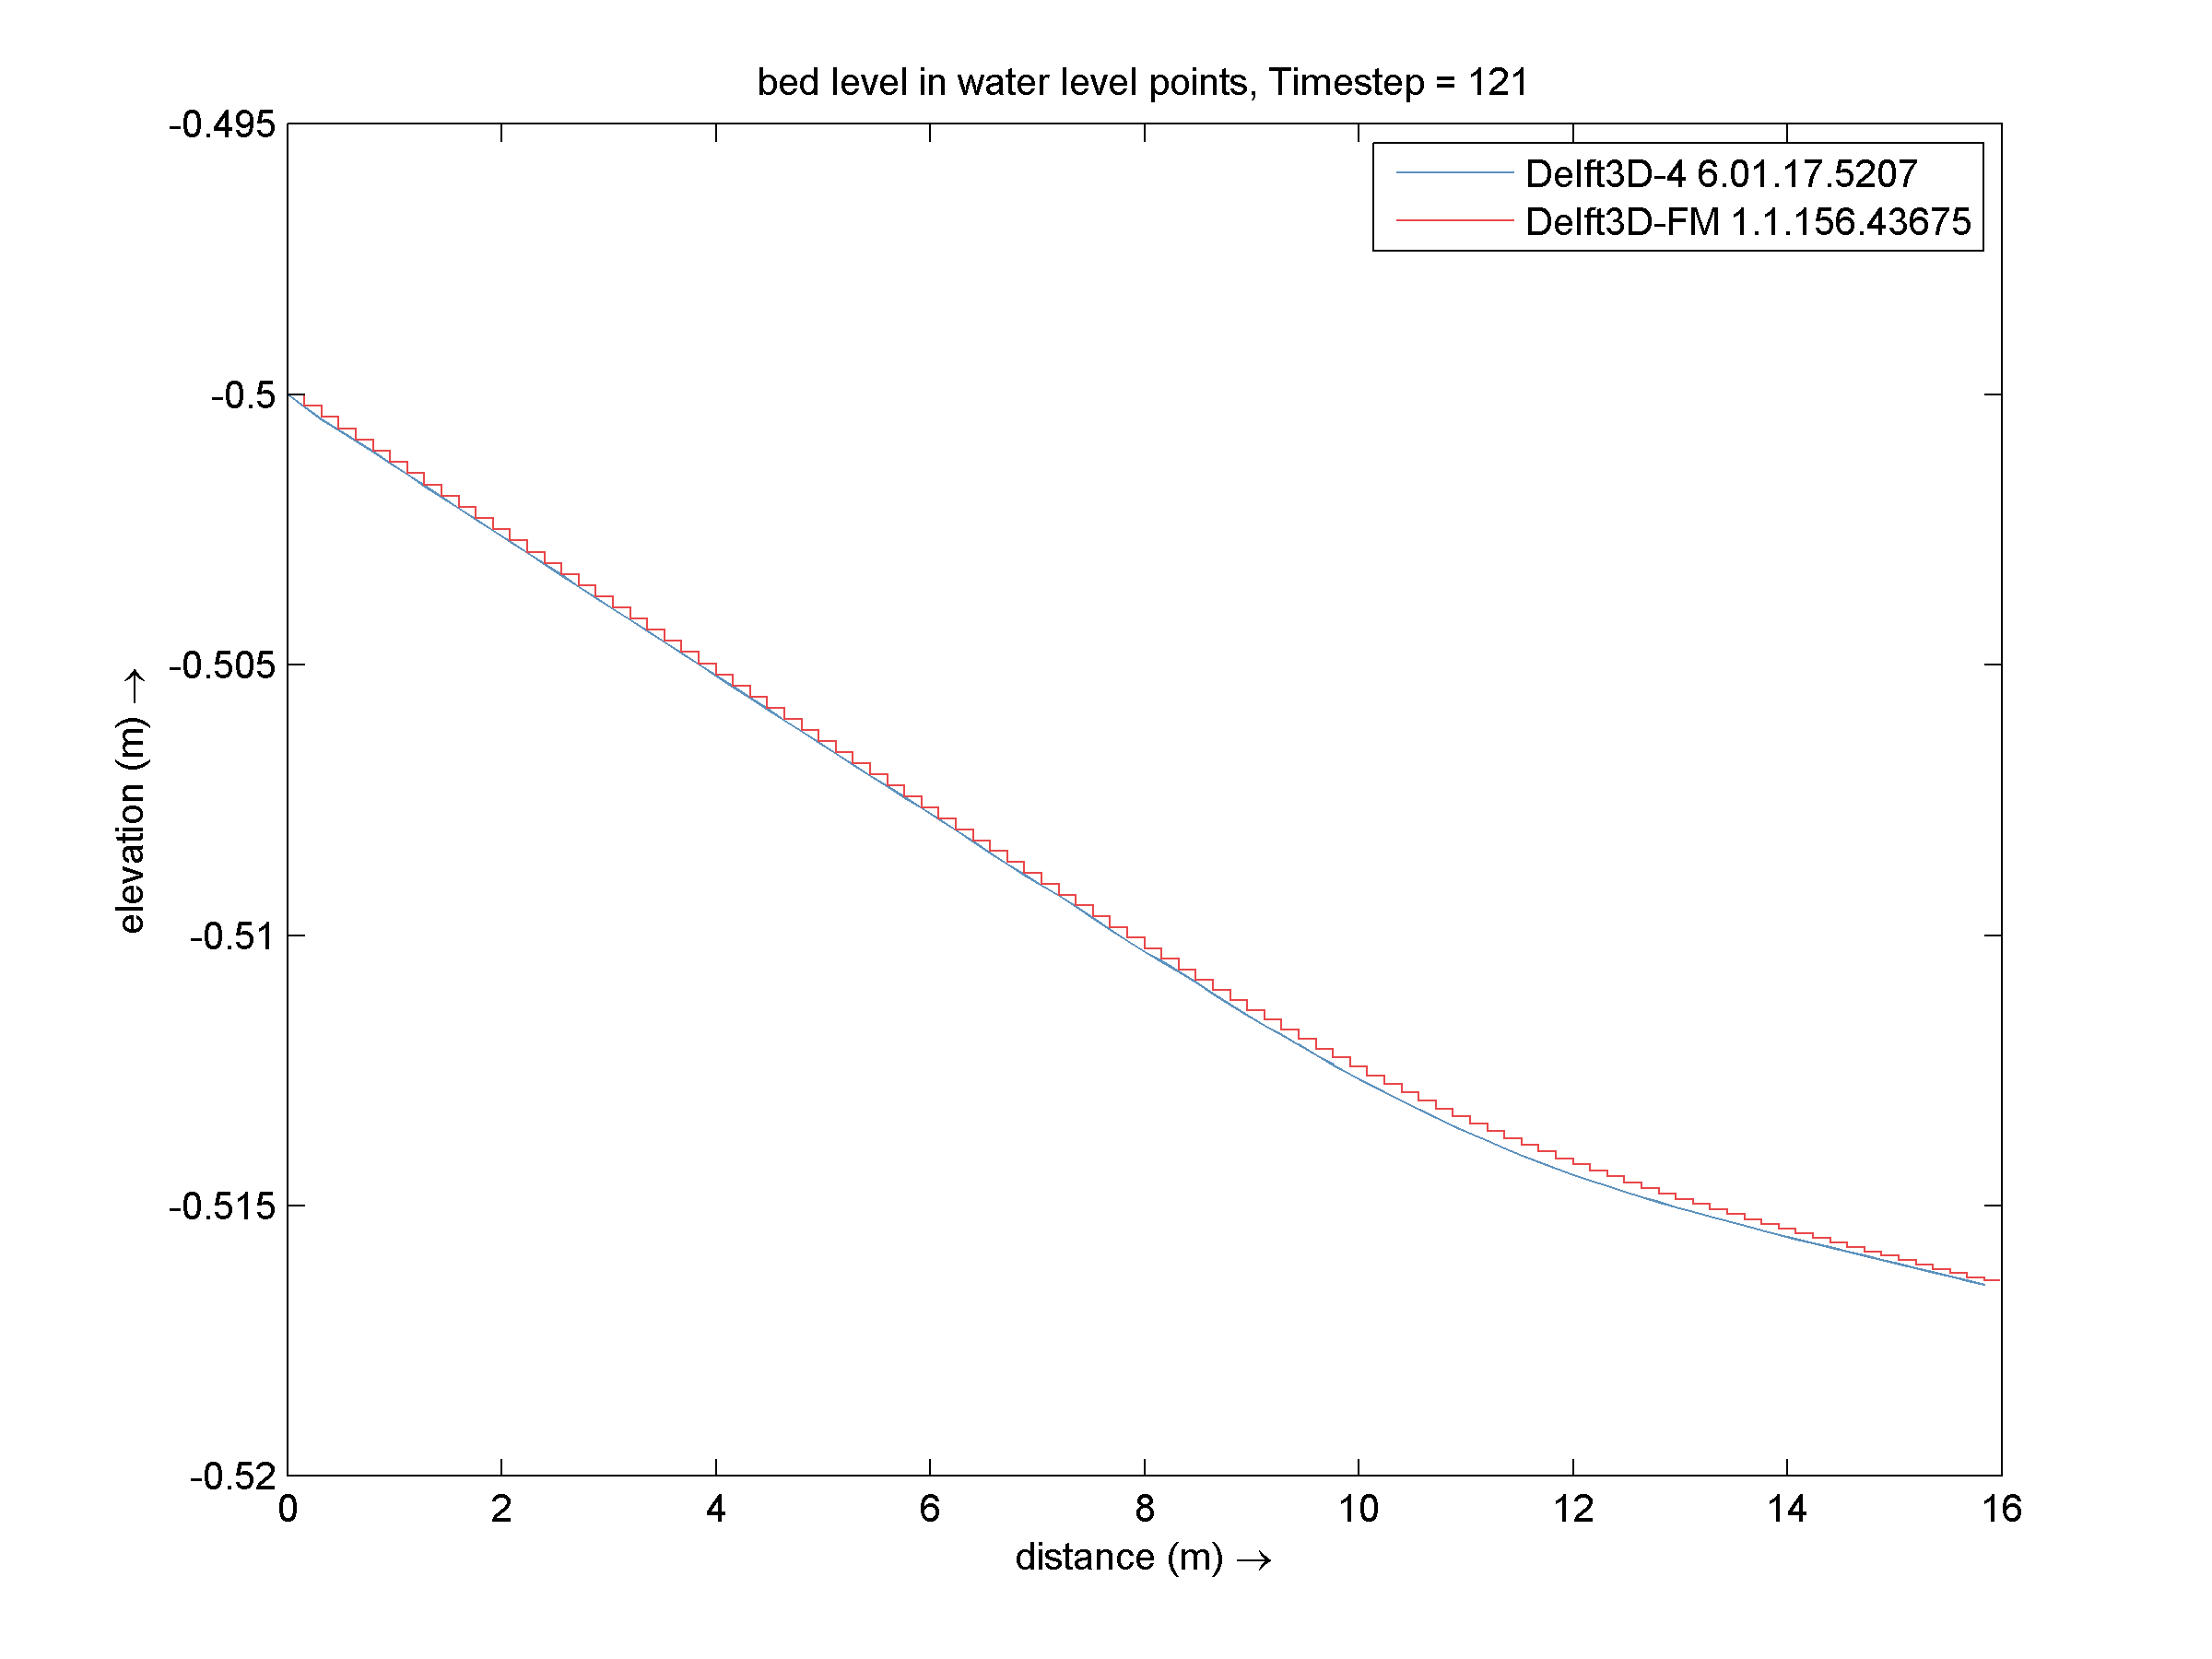
\includegraphics[width=0.70\textwidth]{figures/comparison_d3d_fm_blstr002.png}
	\end{center}
	\caption{Comparison of bed levels ('depth change' = 0).}\label{fig:e02-fxx-cxx:bedlevelstr002}
\end{figure}

\begin{figure}[htb]
	\begin{center}
		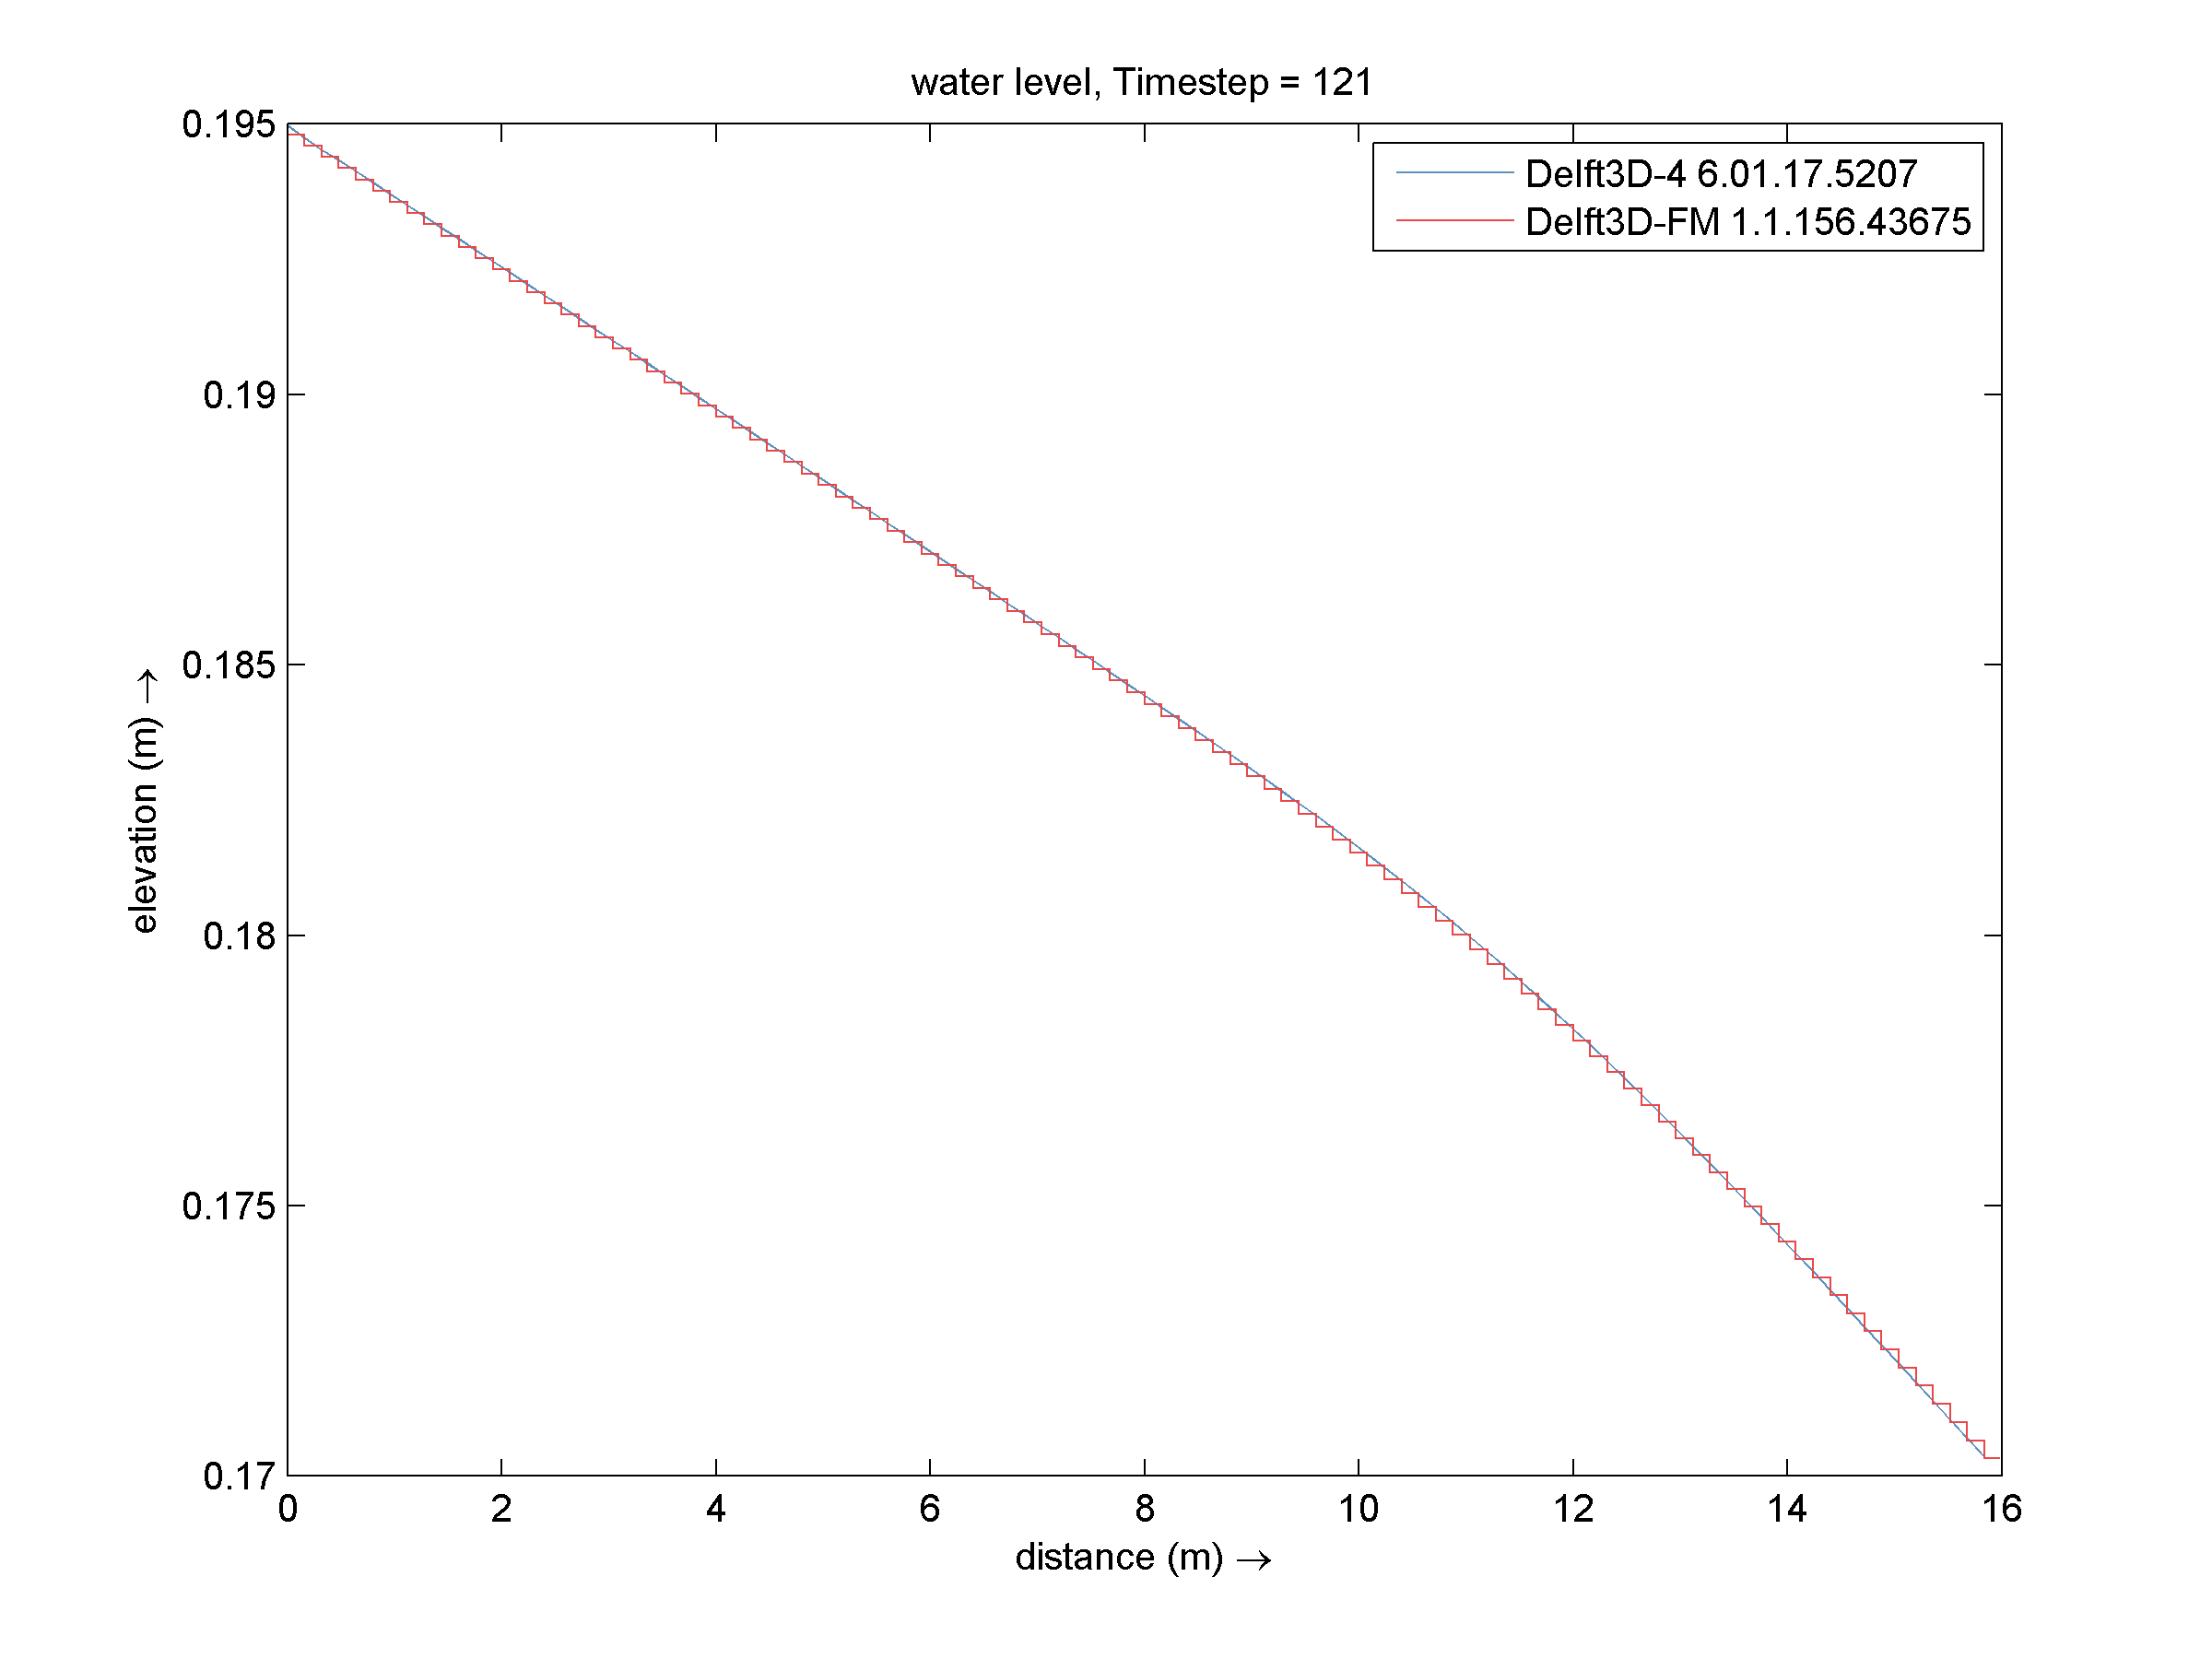
\includegraphics[width=0.70\textwidth]{figures/comparison_d3d_fm_wlstr002.png}
	\end{center}
	\caption{Comparison of water levels ('depth change' = 0).}\label{fig:e02-fxx-cxx:waterlevelstr002}
\end{figure}

\begin{figure}[htb]
	\begin{center}
		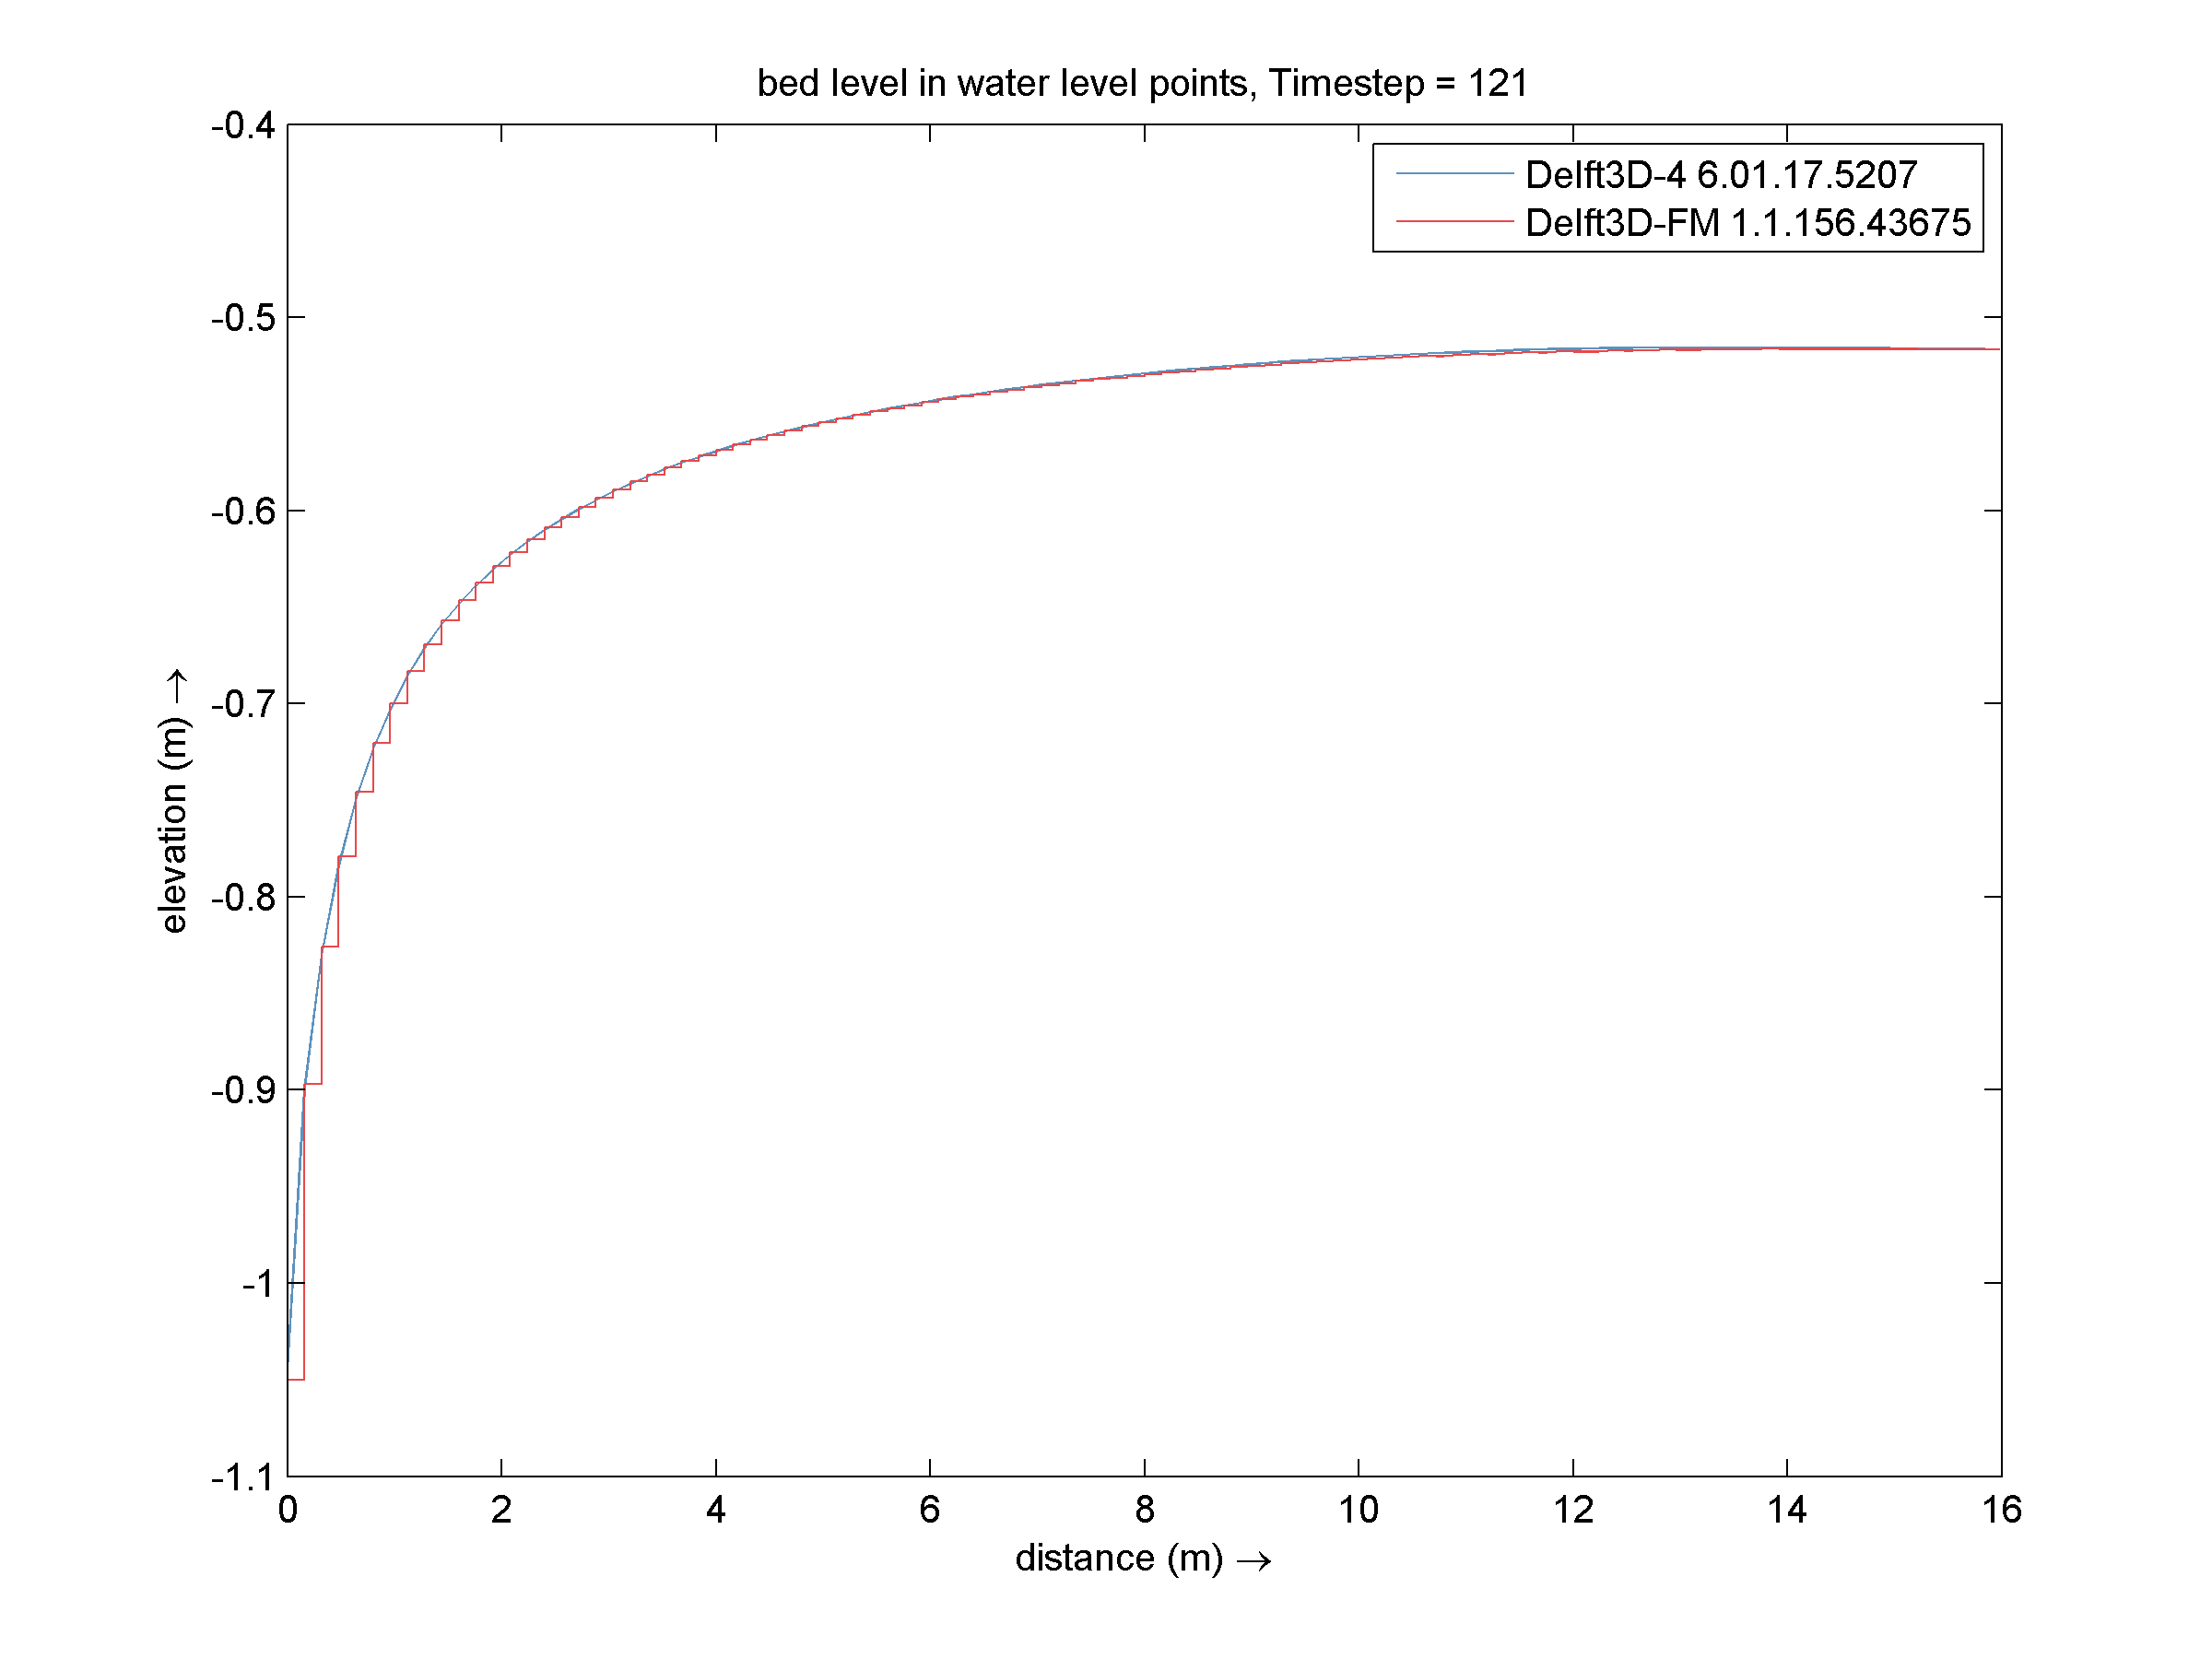
\includegraphics[width=0.70\textwidth]{figures/comparison_d3d_fm_blstr003.png}
	\end{center}
	\caption{Comparison of bed levels ('transport with pores' = 0).}\label{fig:e02-fxx-cxx:bedlevelstr003}
\end{figure}

\begin{figure}[htb]
	\begin{center}
		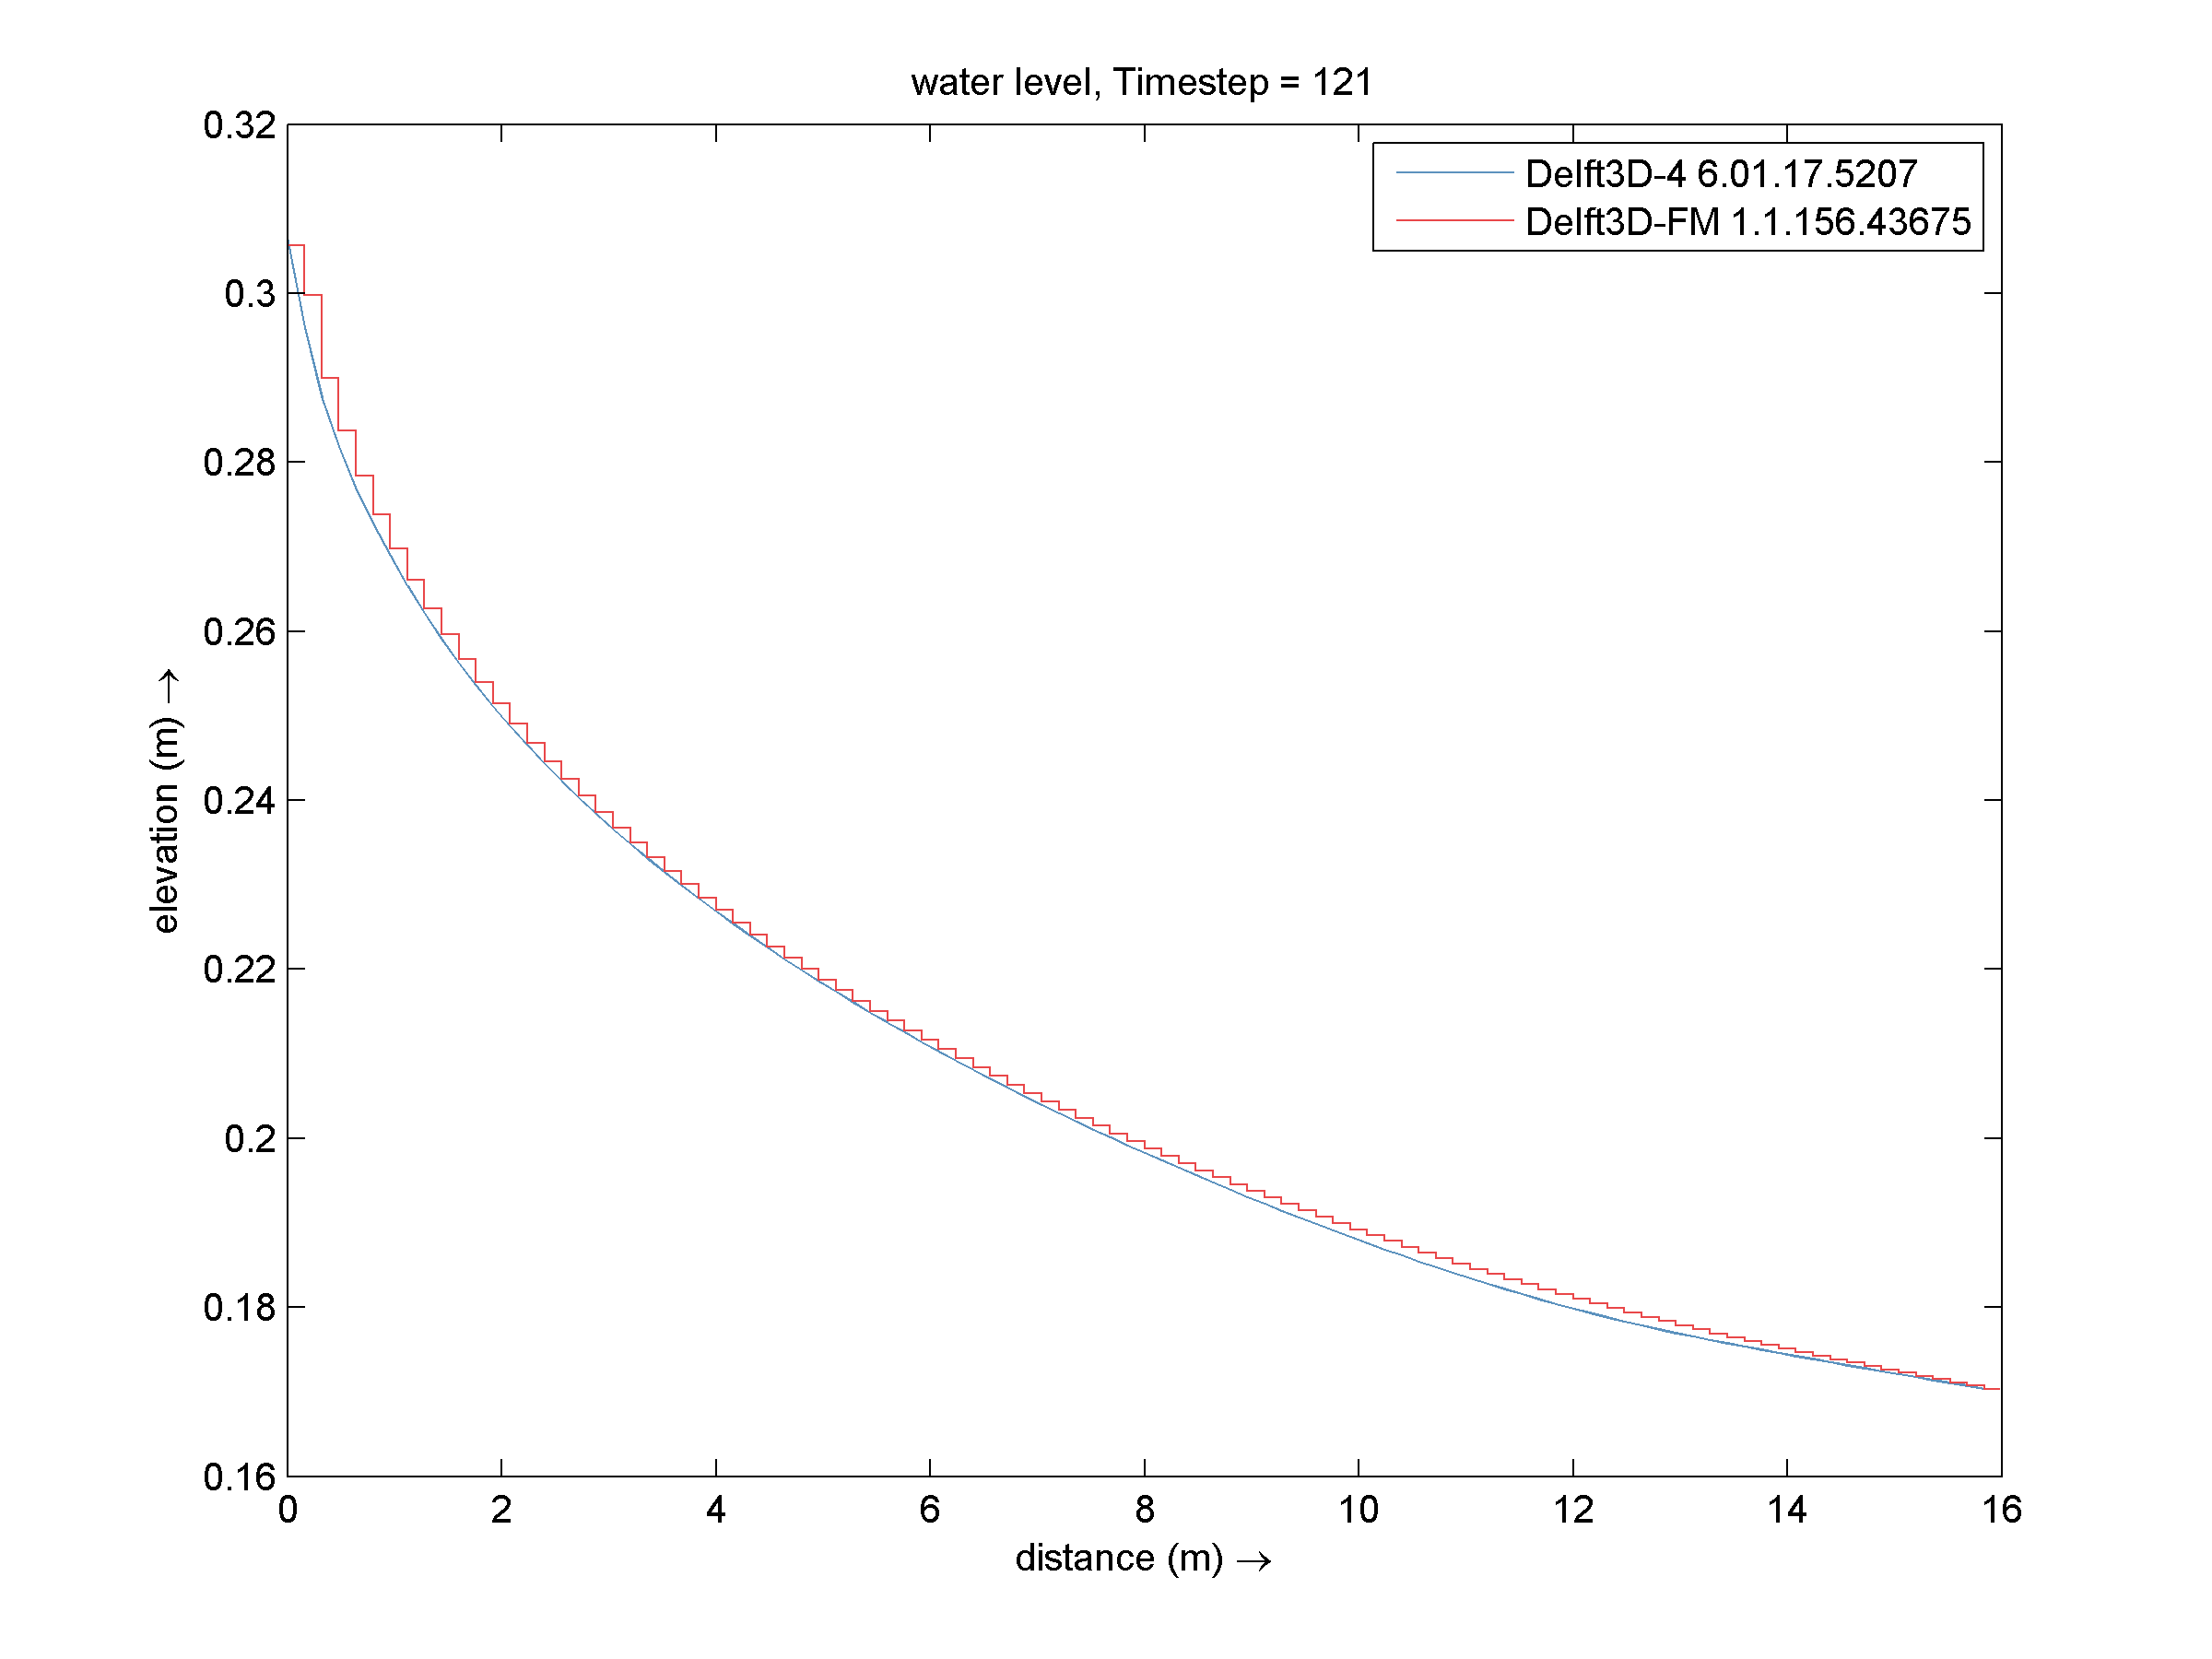
\includegraphics[width=0.70\textwidth]{figures/comparison_d3d_fm_wlstr003.png}
	\end{center}
	\caption{Comparison of water levels ('transport with pores' = 0).}\label{fig:e02-fxx-cxx:waterlevelstr003}
\end{figure}

\begin{figure}[htb]
	\begin{center}
		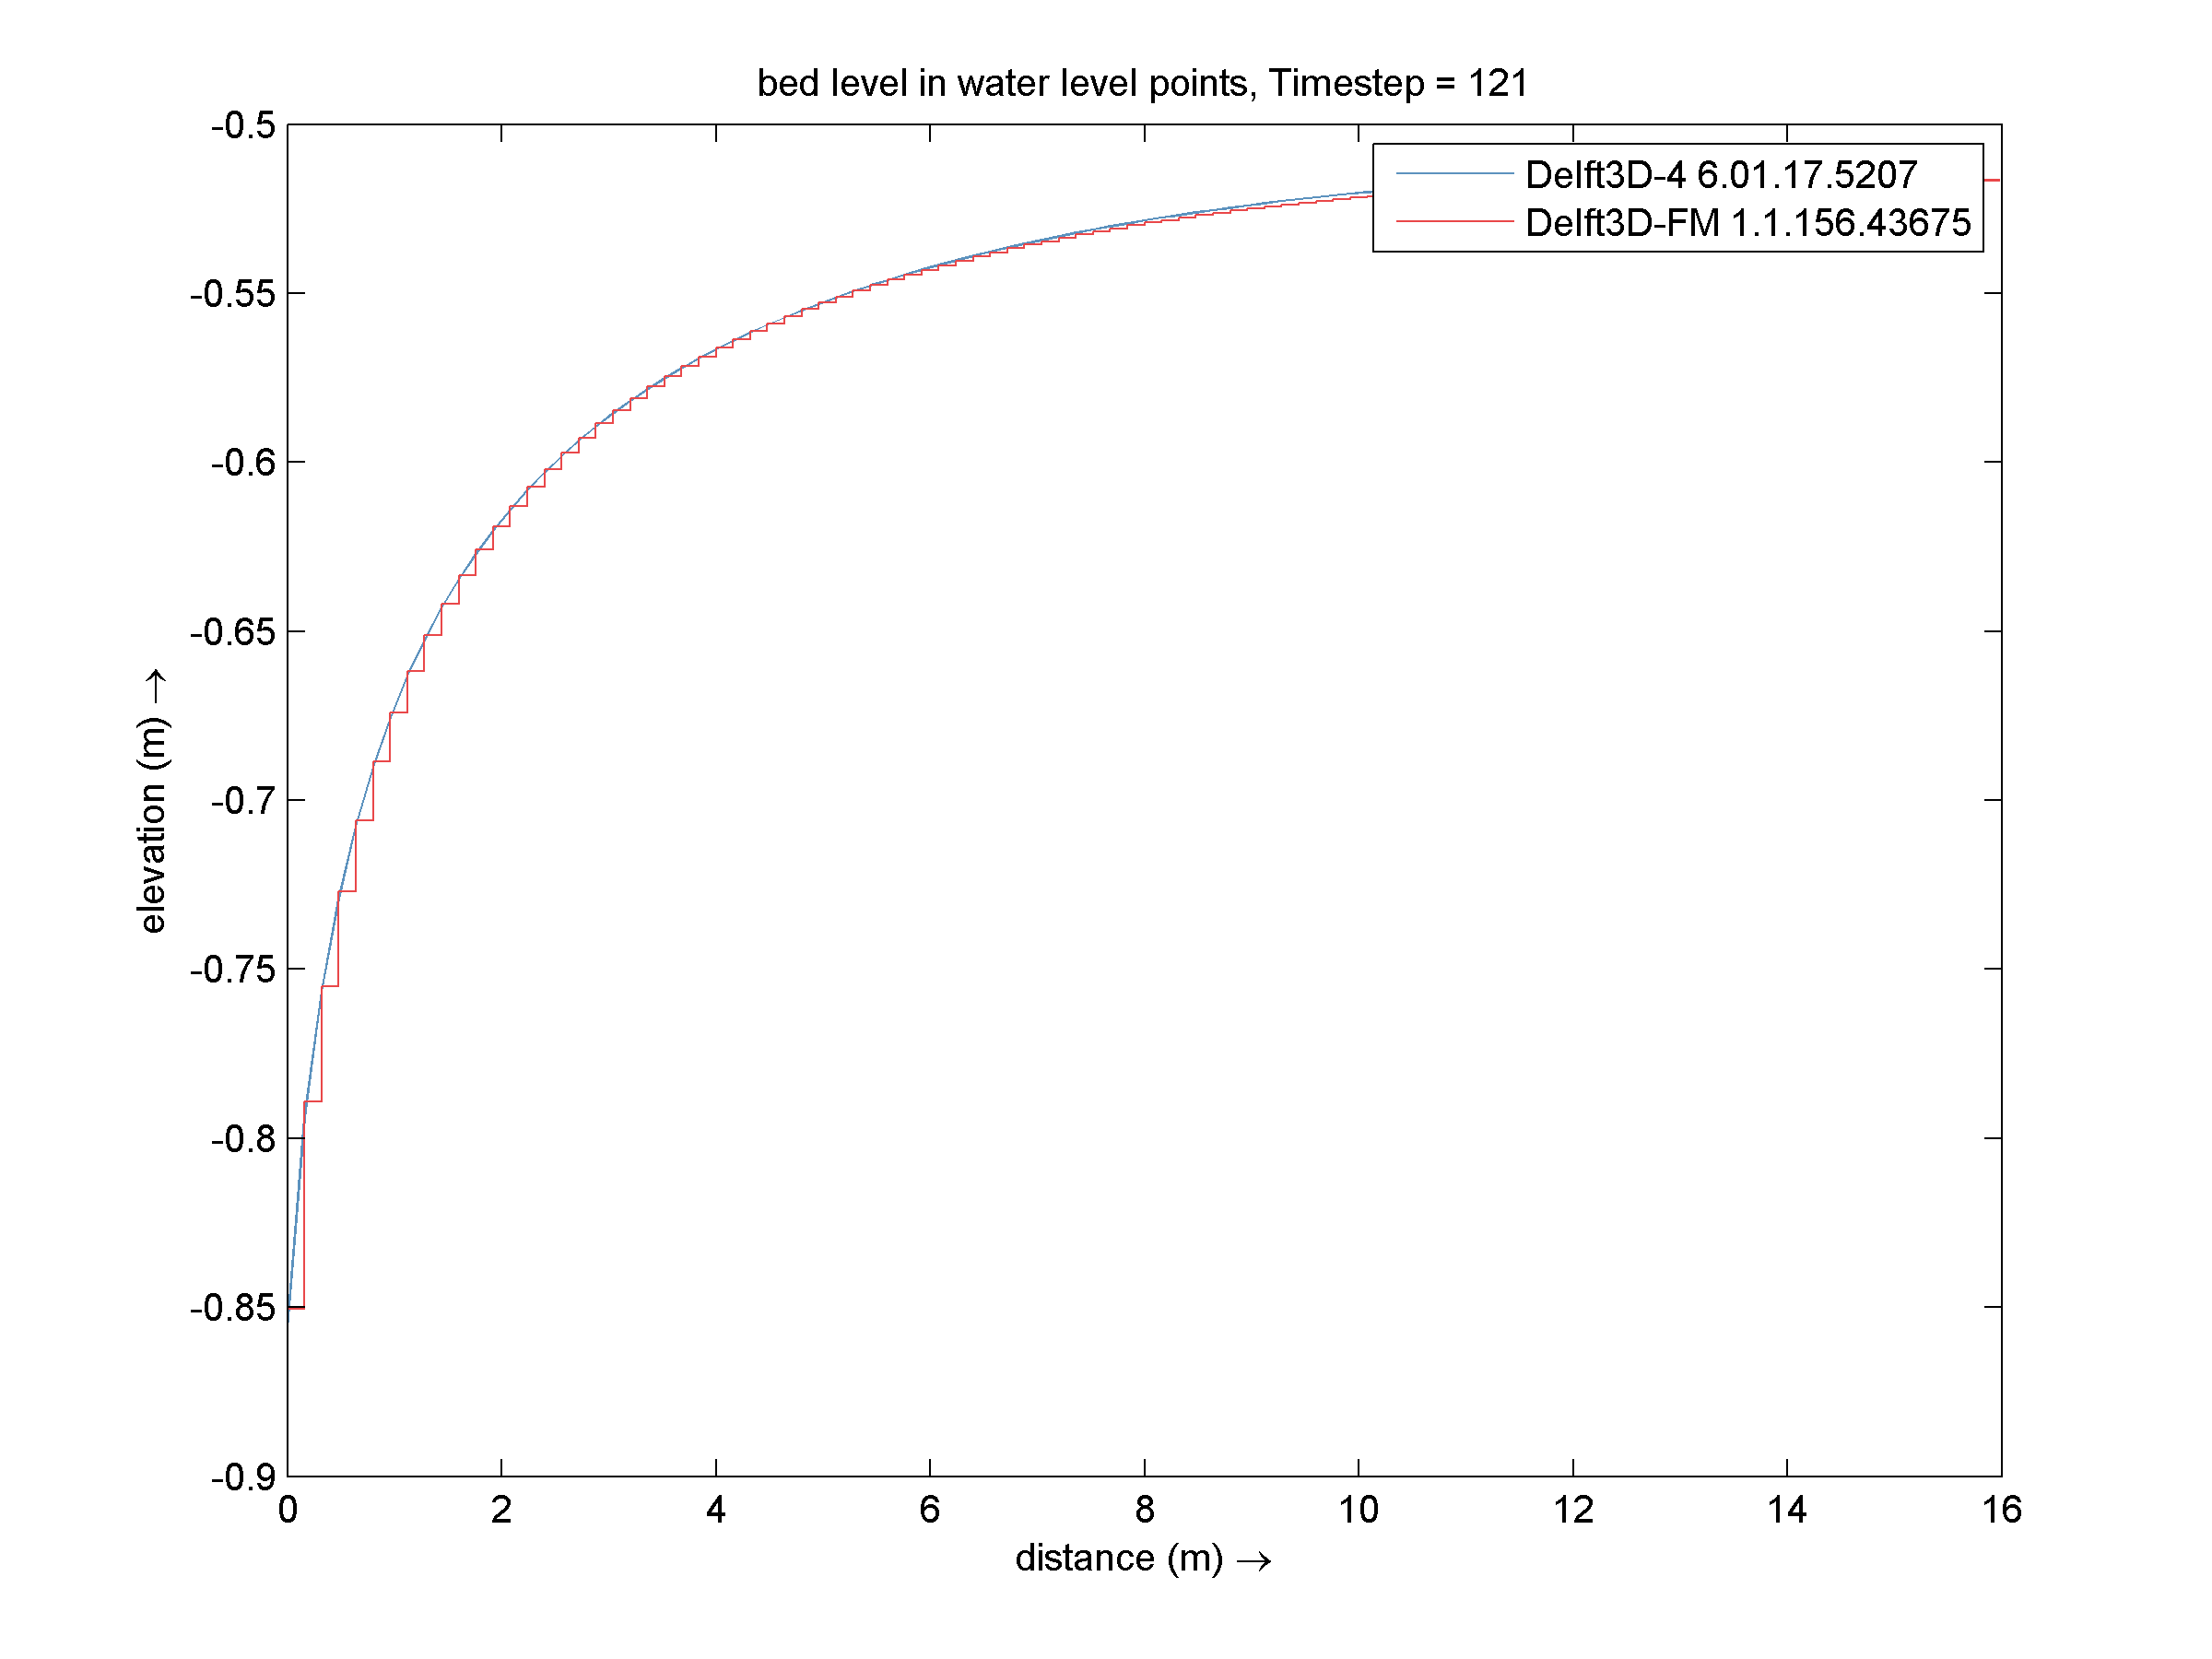
\includegraphics[width=0.70\textwidth]{figures/comparison_d3d_fm_blstr2.png}
	\end{center}
	\caption{Comparison of bed levels ('depth' changes from -0.5 to -1 m).}\label{fig:e02-fxx-cxx:bedlevelstr2}
\end{figure}

\begin{figure}[htb]
	\begin{center}
		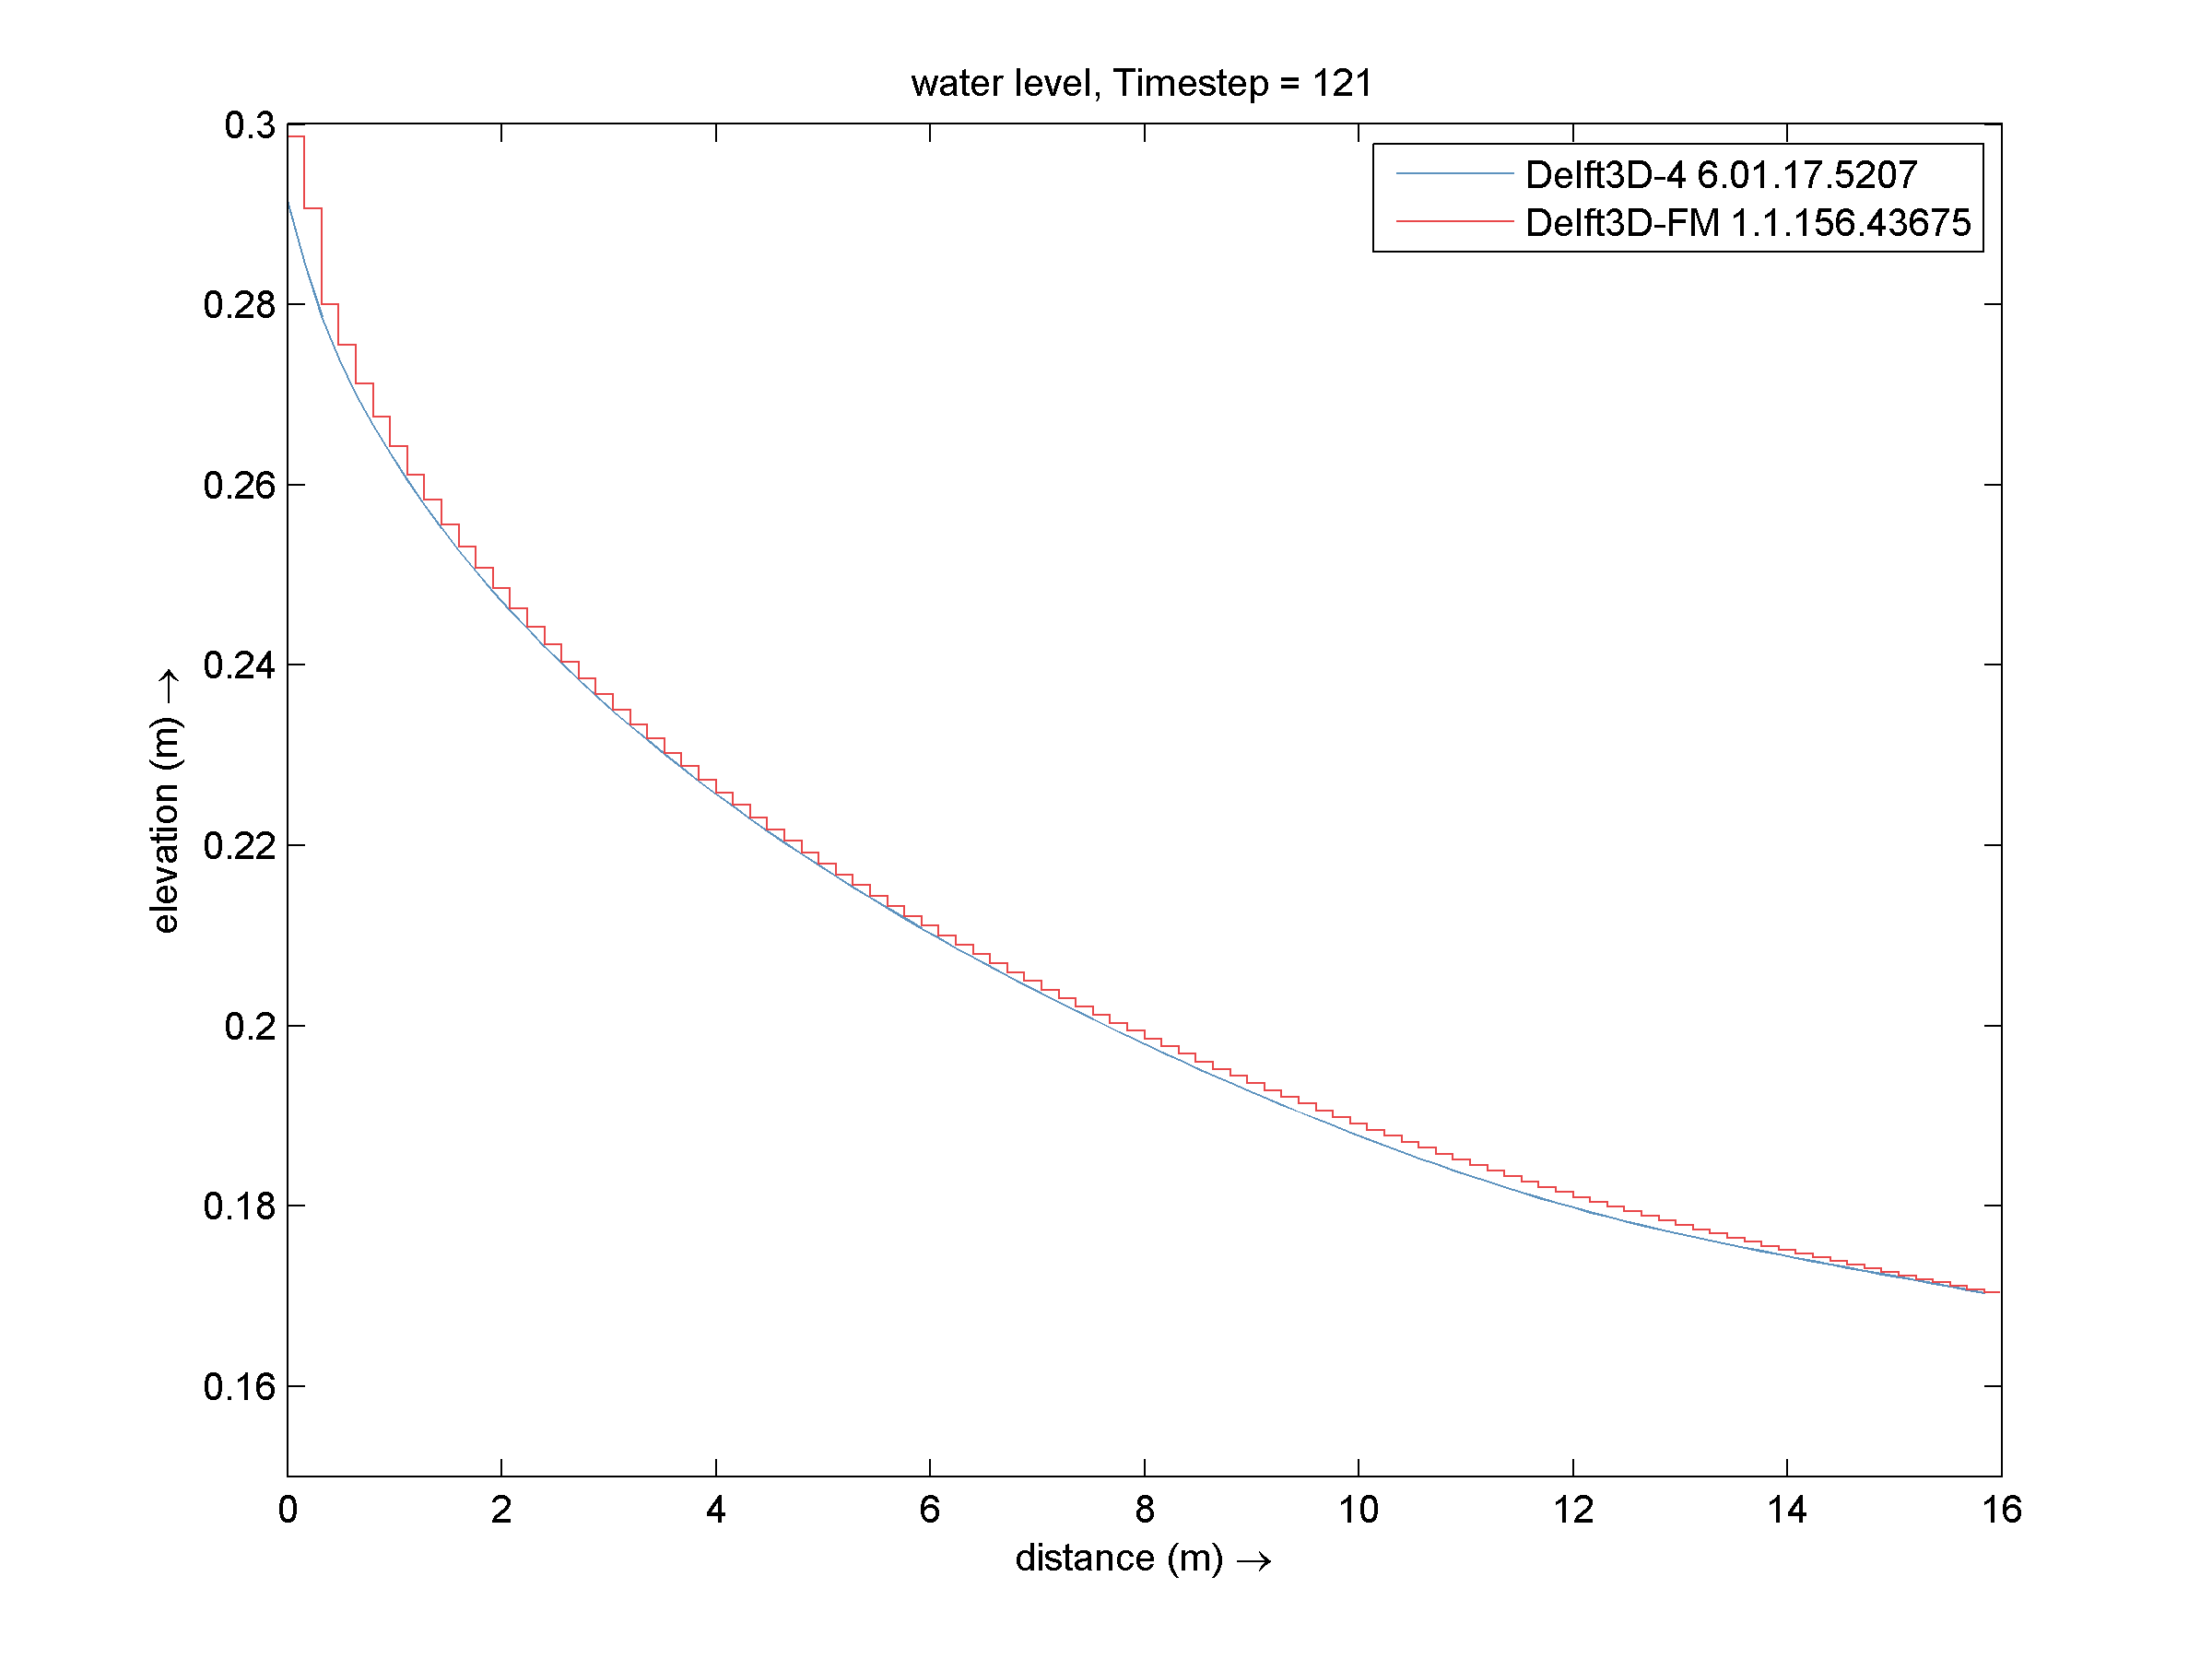
\includegraphics[width=0.70\textwidth]{figures/comparison_d3d_fm_wlstr2.png}
	\end{center}
	\caption{Comparison of water levels ('depth' changes from -0.5 to -1 m).}\label{fig:e02-fxx-cxx:waterlevelstr2}
\end{figure}

\begin{figure}[htb]
	\begin{center}
		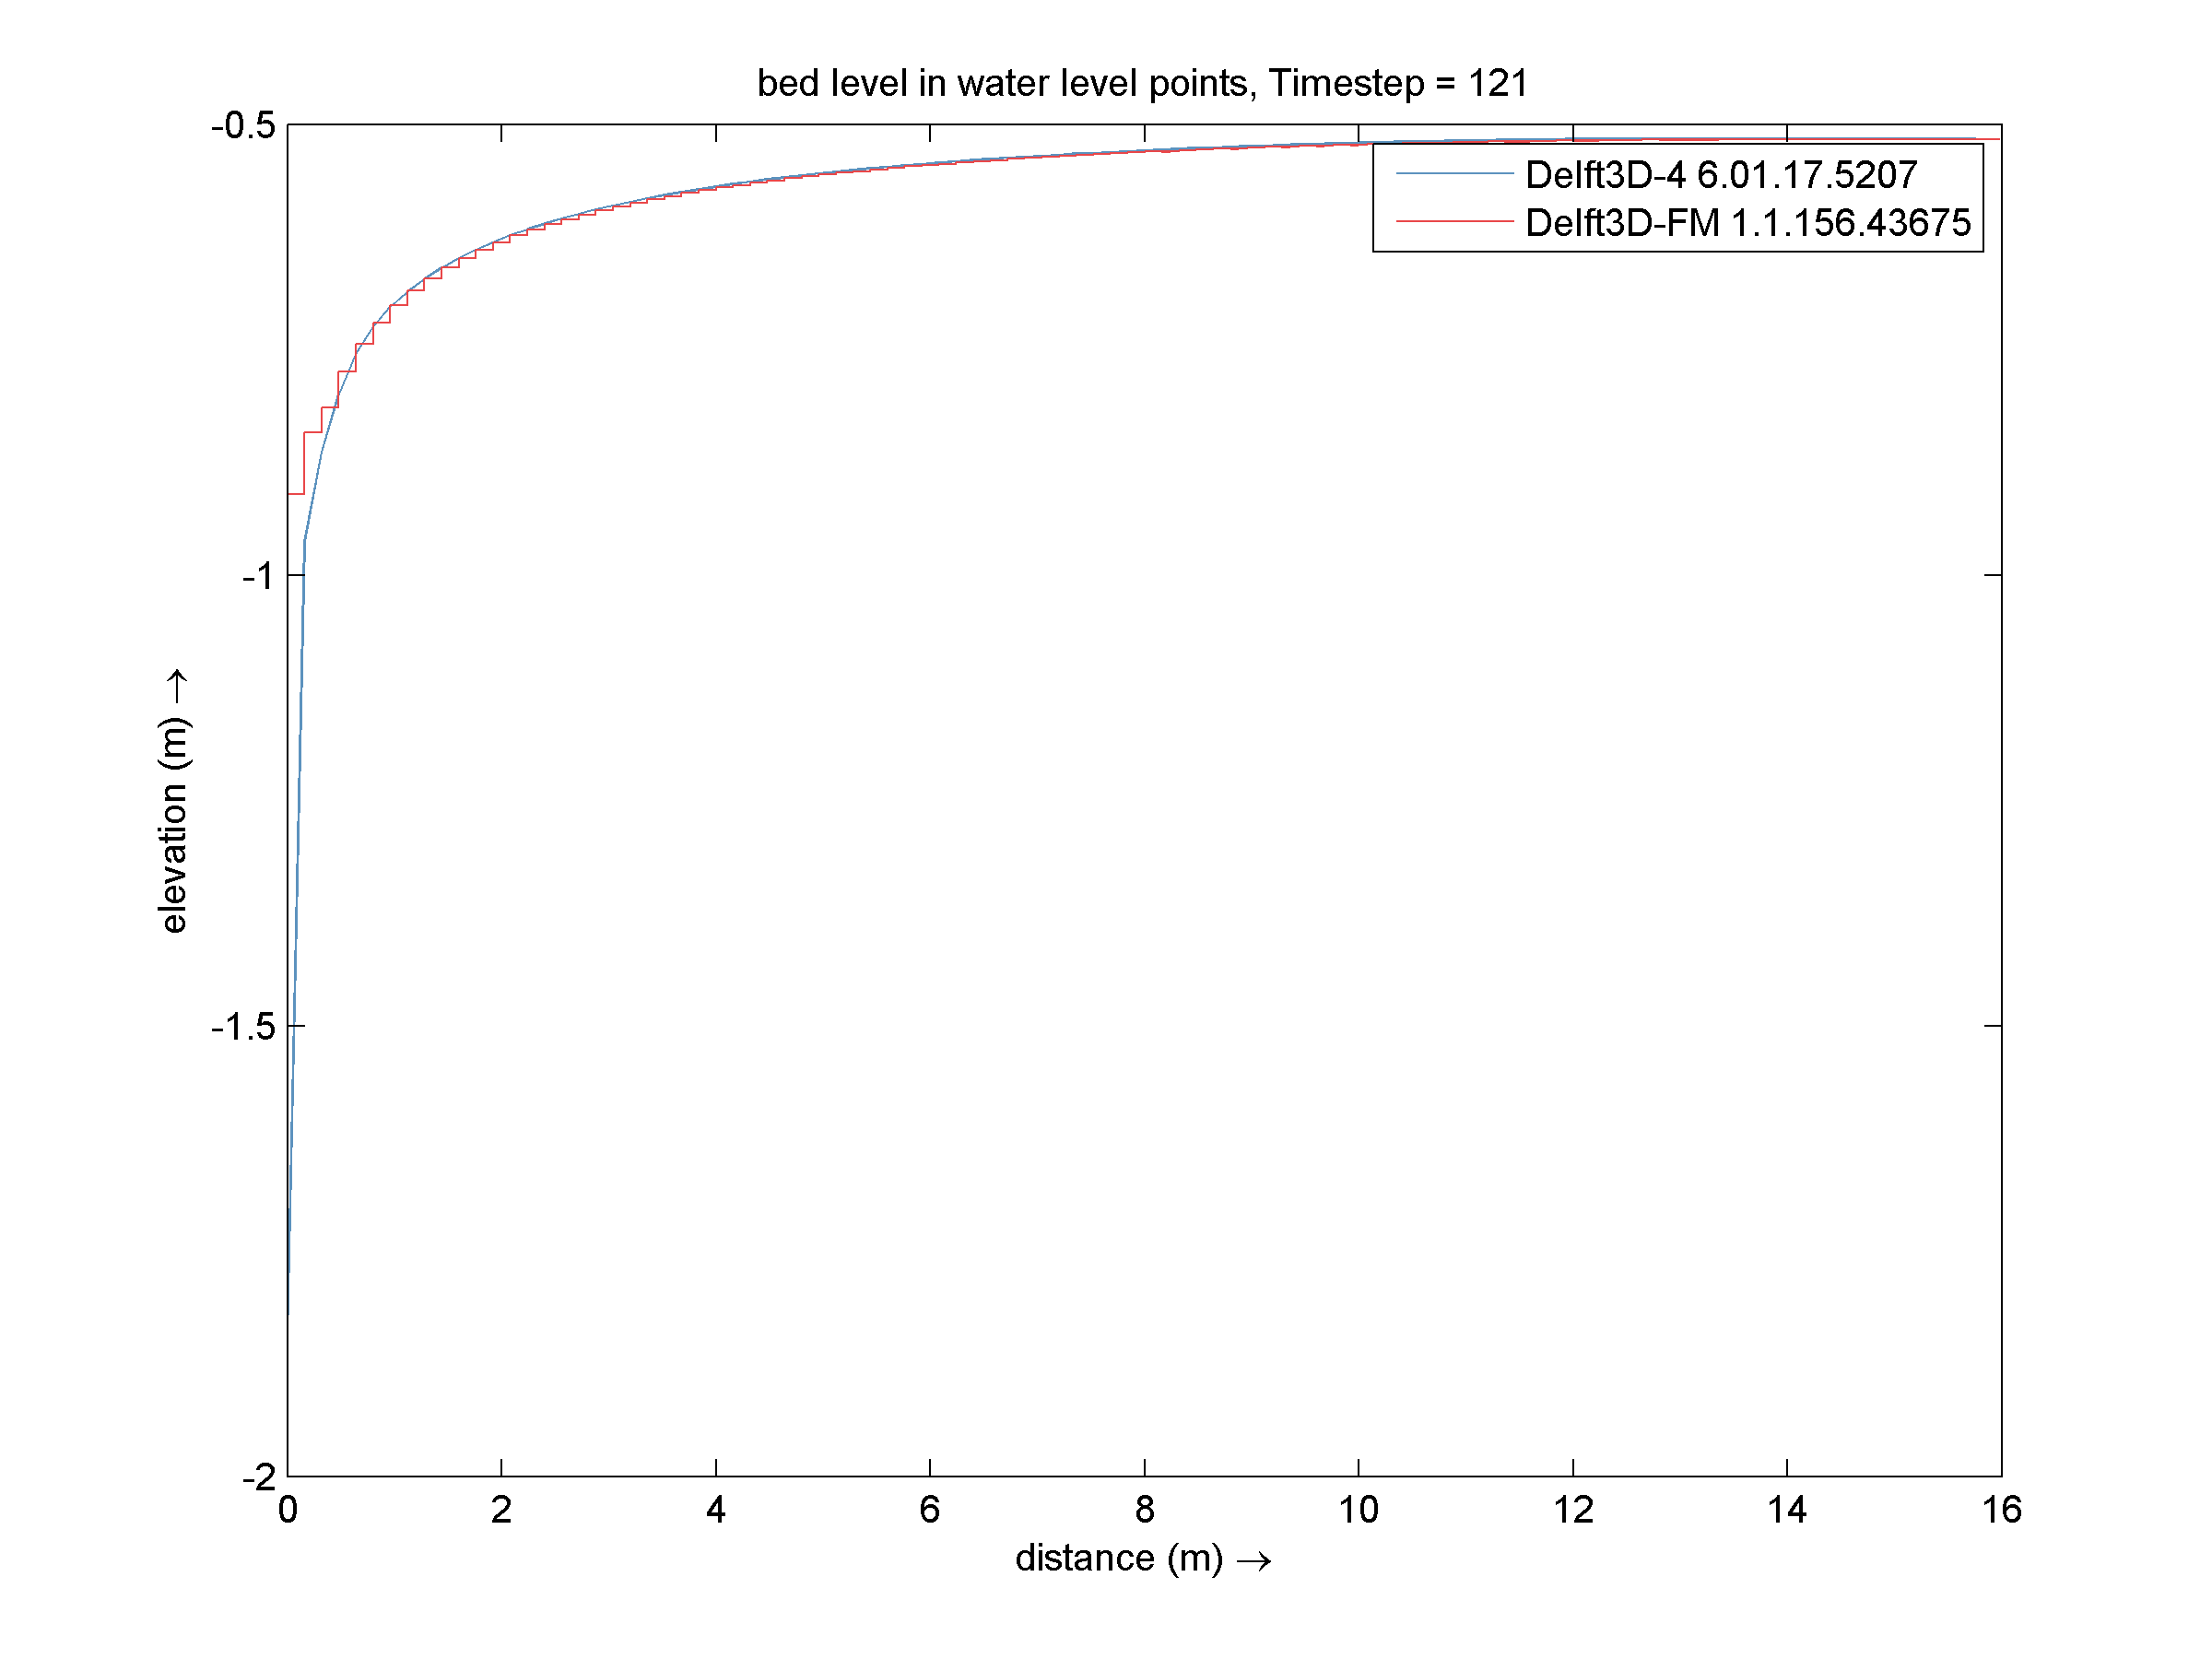
\includegraphics[width=0.70\textwidth]{figures/comparison_d3d_fm_blstr3.png}
	\end{center}
	\caption{Comparison of bed levels('depth change' changes from 0 to -0.5 m).}\label{fig:e02-fxx-cxx:bedlevelstr3}
\end{figure}

\begin{figure}[htb]
	\begin{center}
		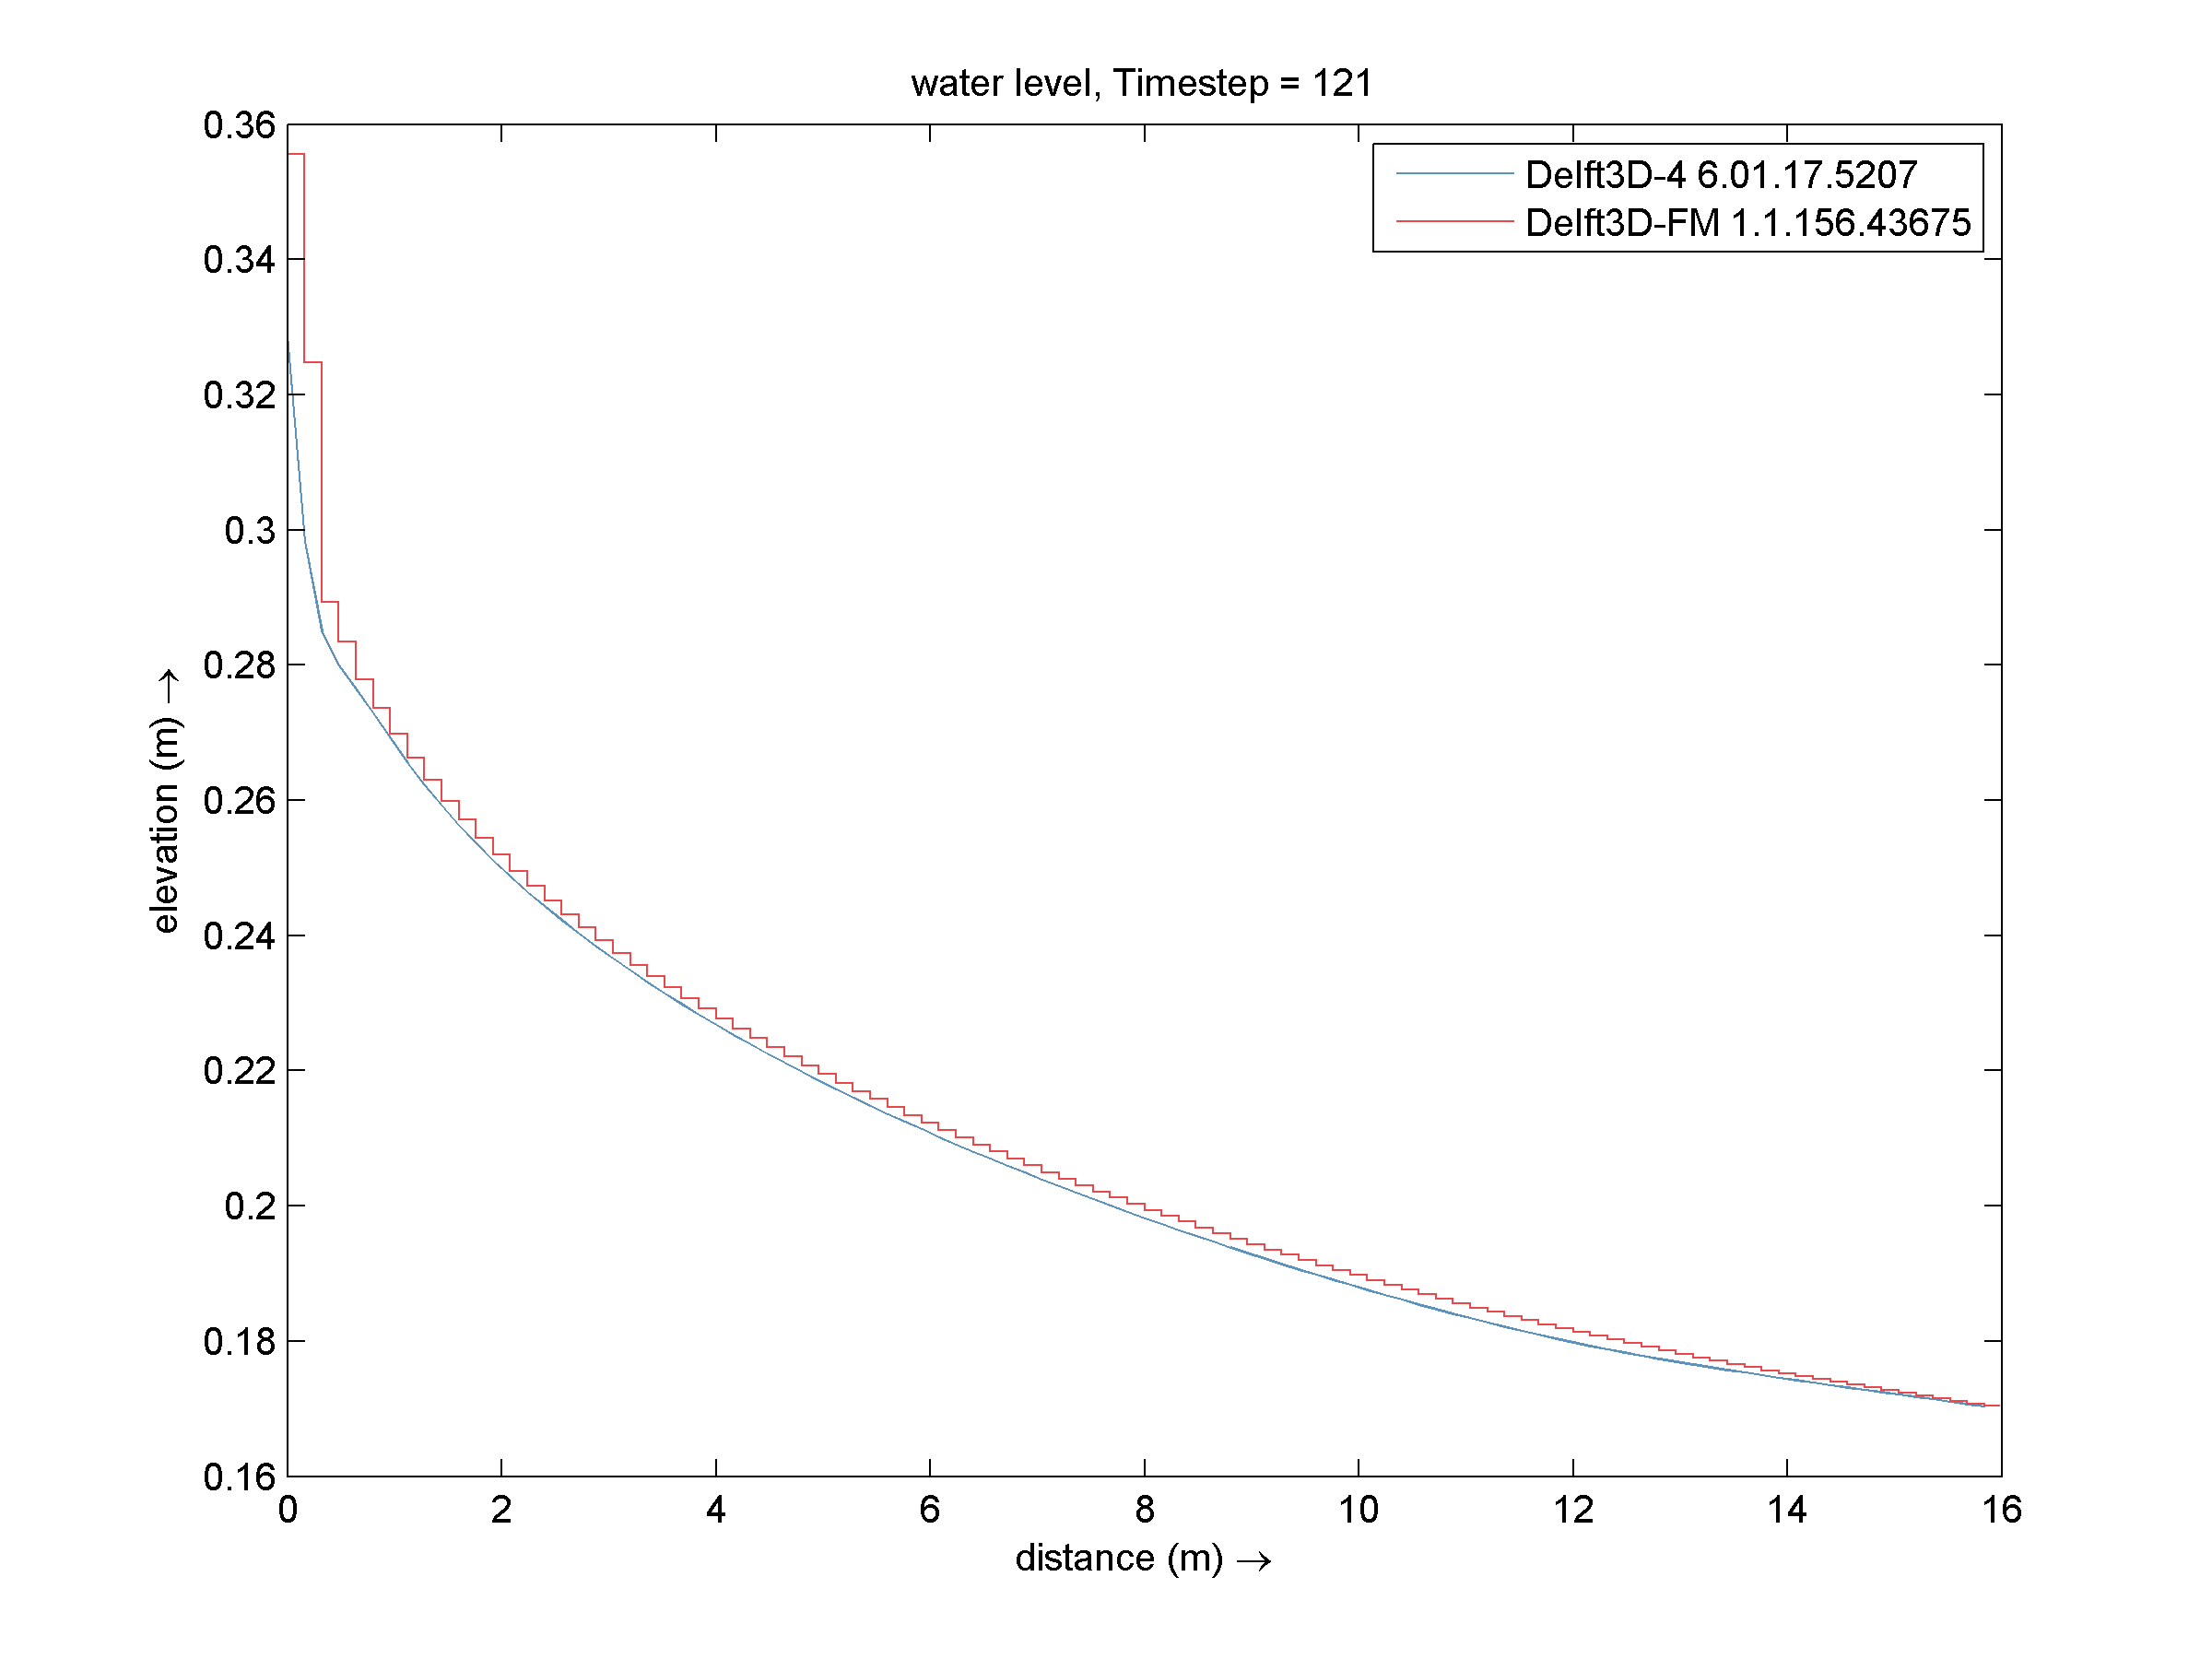
\includegraphics[width=0.70\textwidth]{figures/comparison_d3d_fm_wlstr3.png}
	\end{center}
	\caption{Comparison of water levels ('depth change' changes from 0 to -0.5 m).}\label{fig:e02-fxx-cxx:waterlevelstr3}
\end{figure}

\begin{figure}[htb]
	\begin{center}
		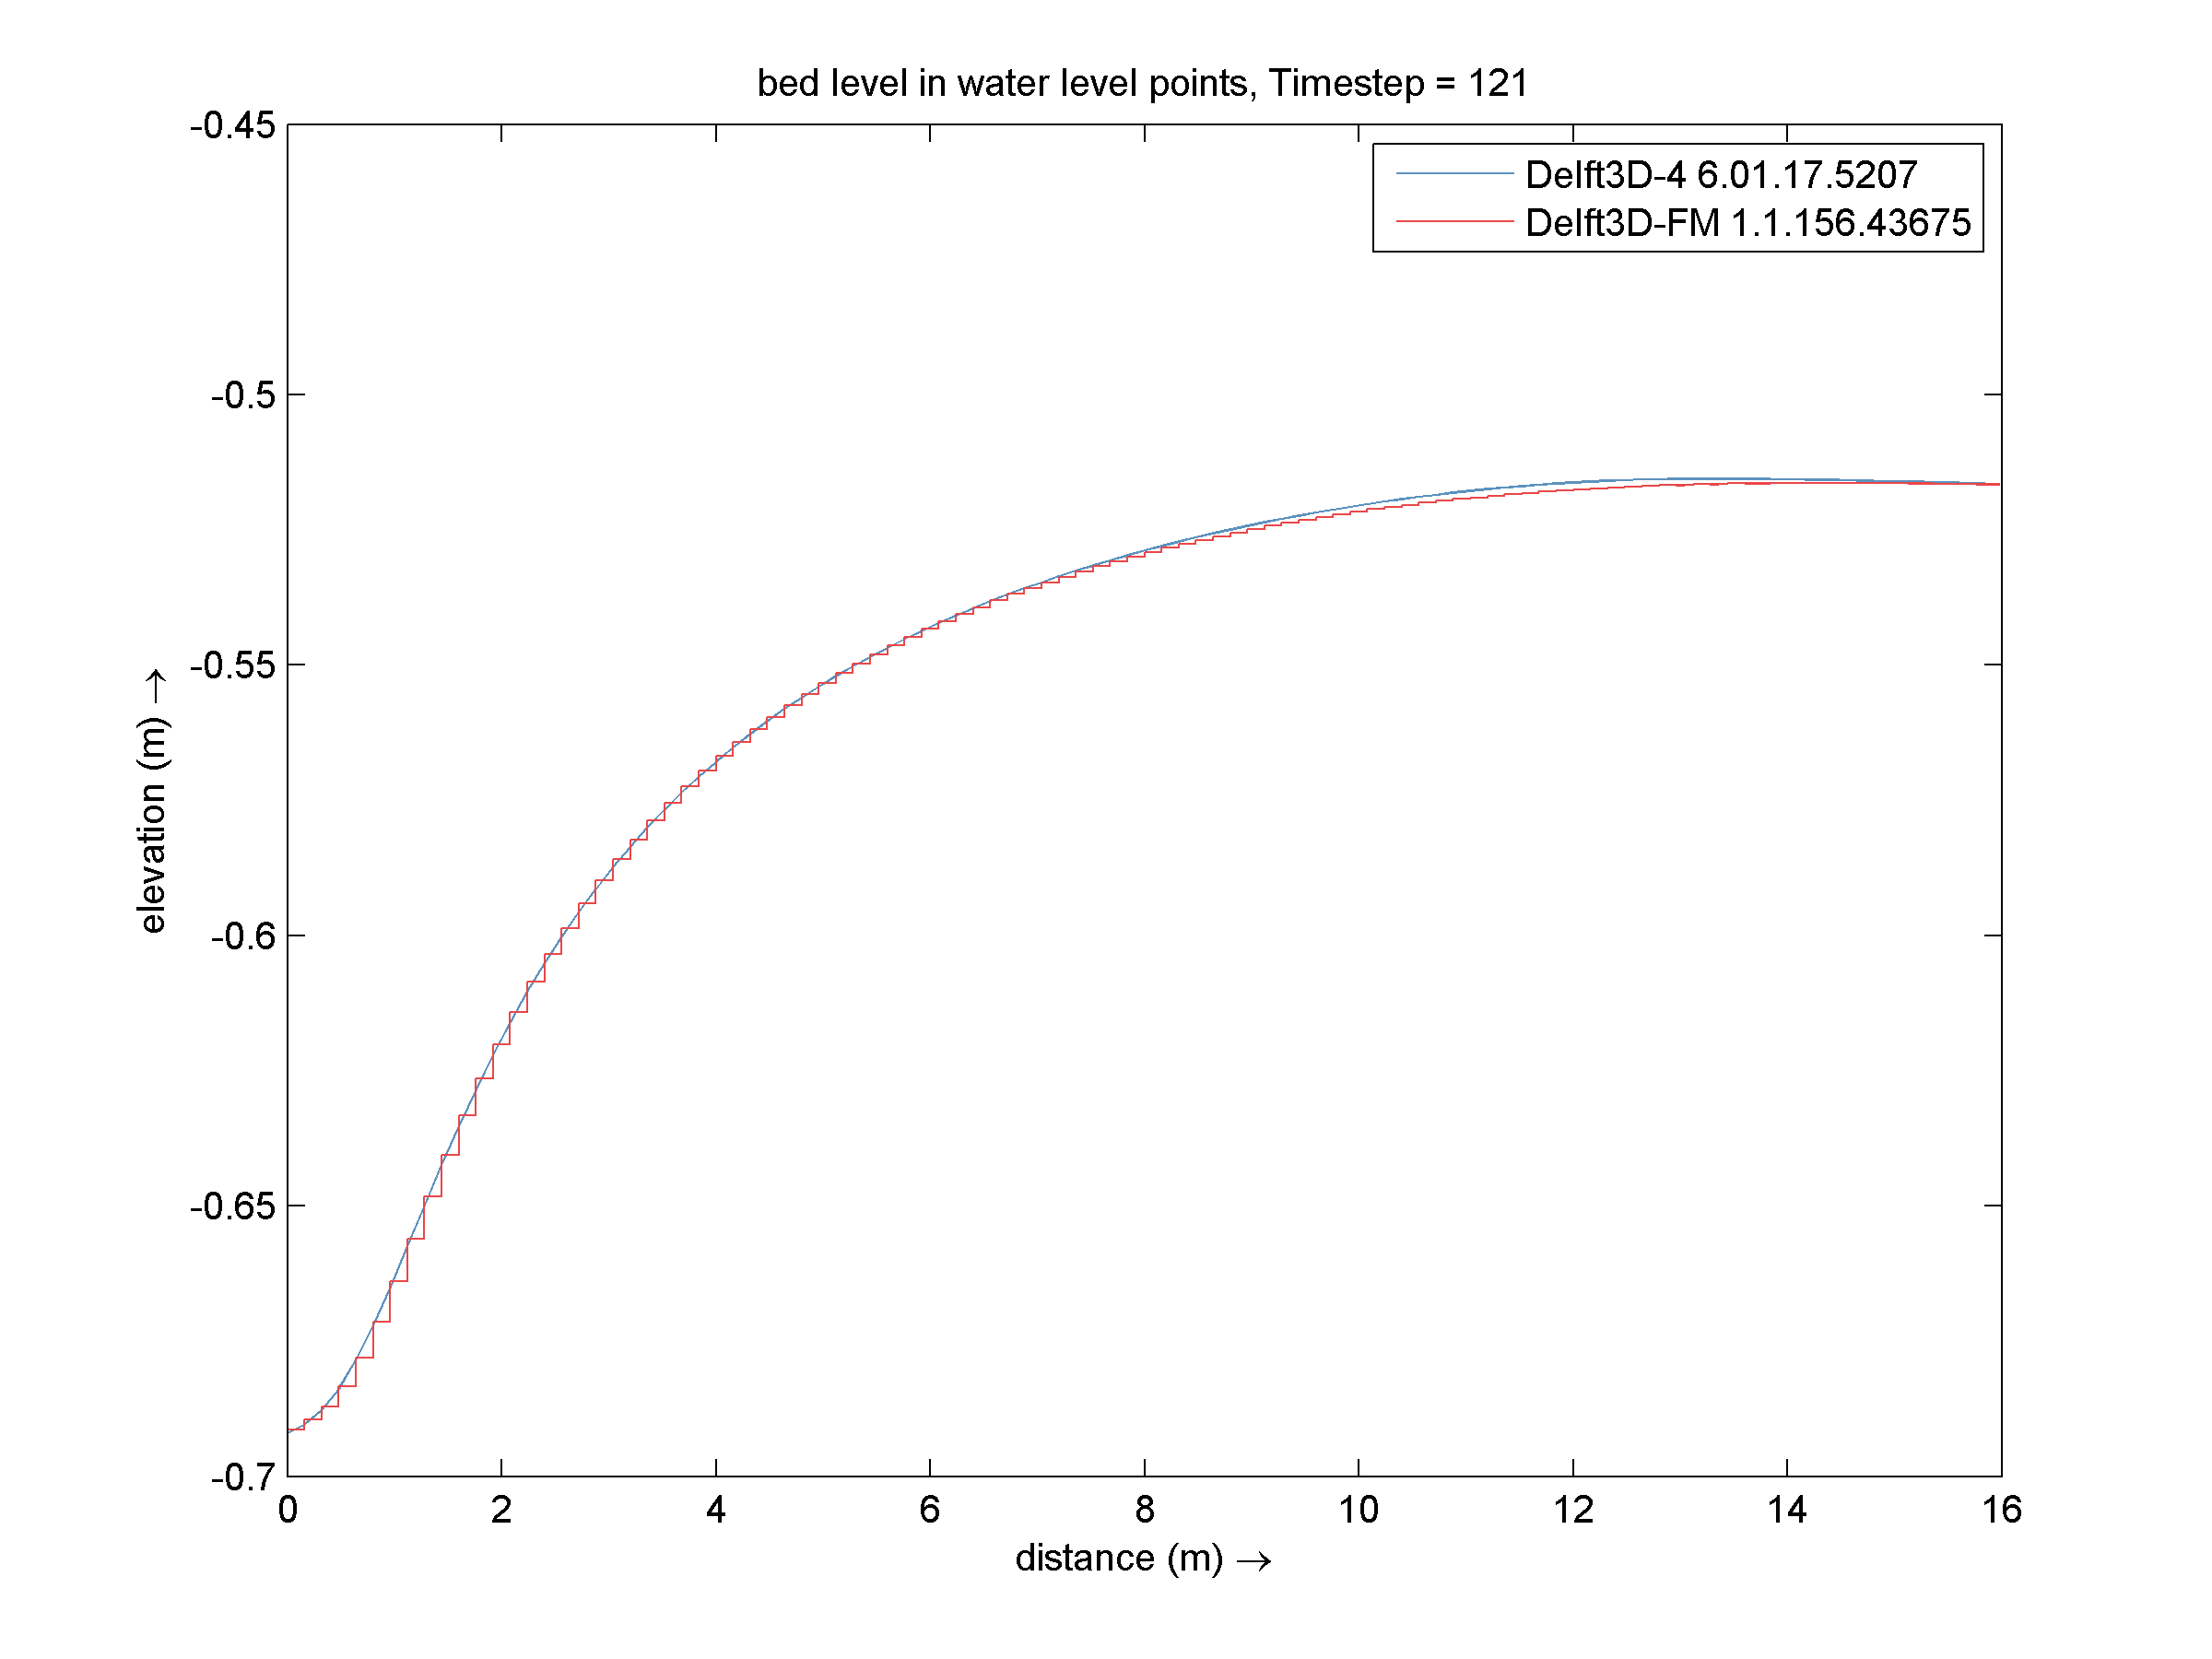
\includegraphics[width=0.70\textwidth]{figures/comparison_d3d_fm_blstr4.png}
	\end{center}
	\caption{Comparison of bed levels ('transport including pores' = 0.0002 m$^2$/s).}\label{fig:e02-fxx-cxx:bedlevelstr4}
\end{figure}

\begin{figure}[htb]
	\begin{center}
		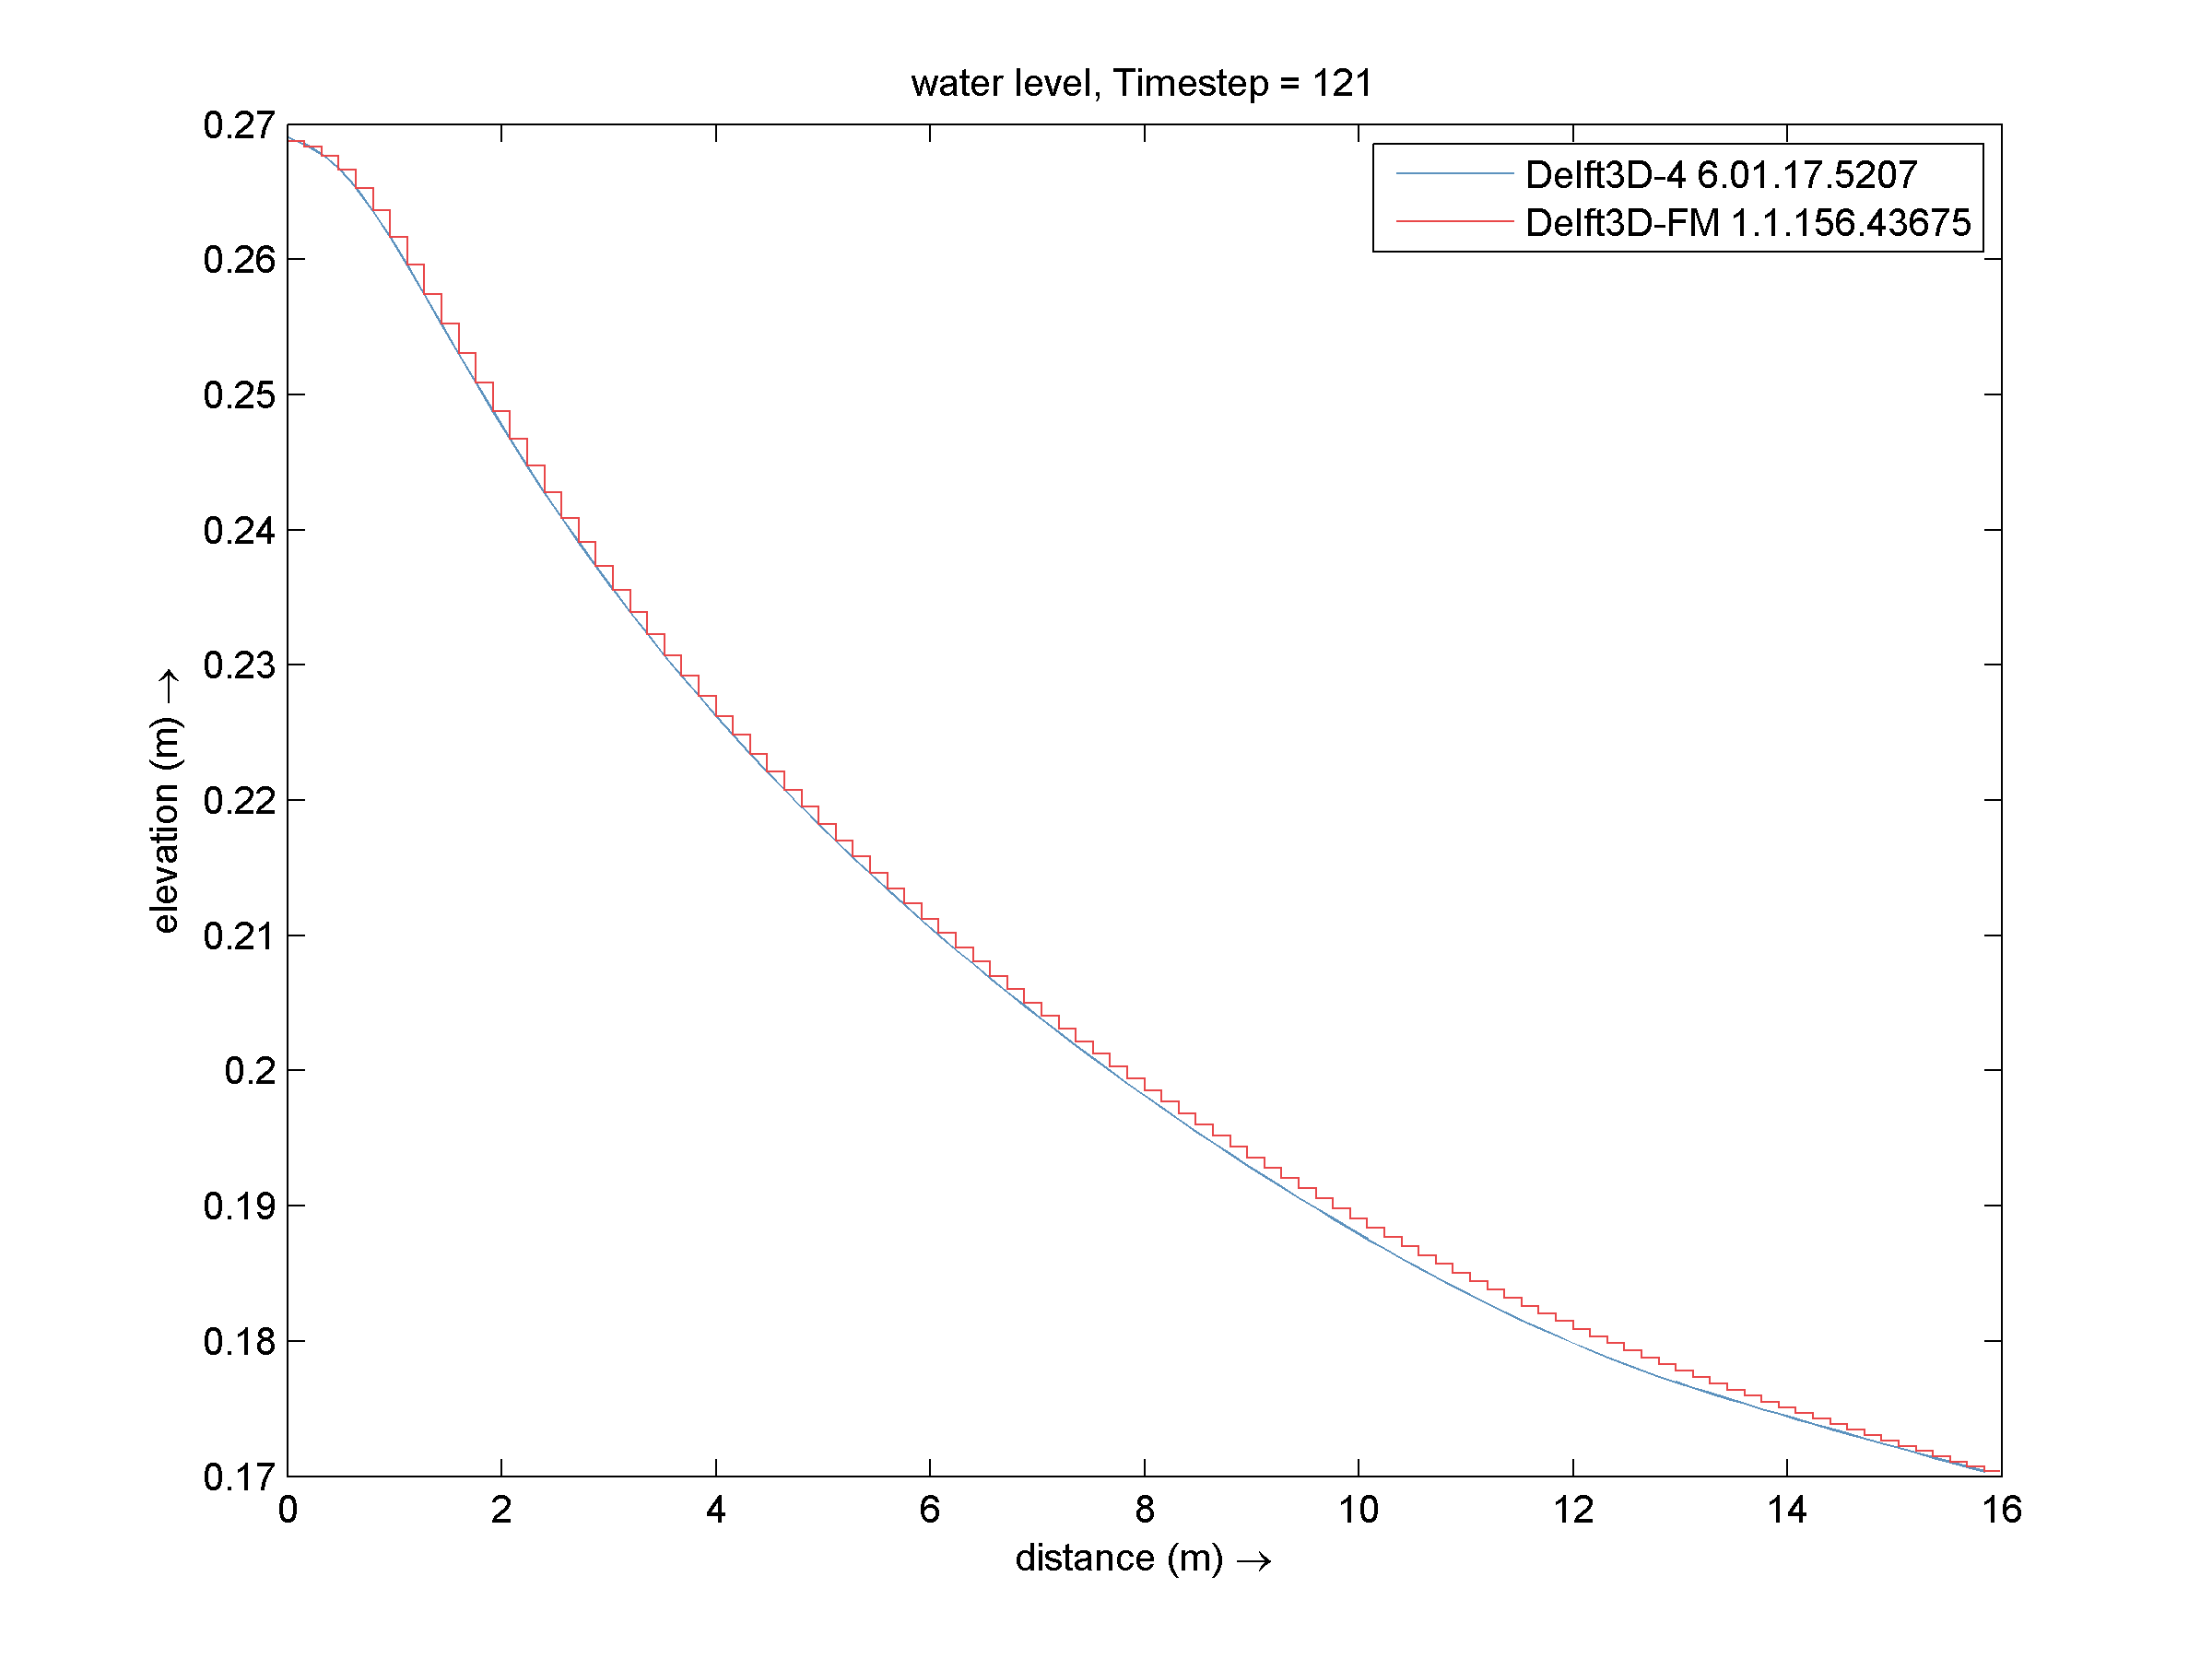
\includegraphics[width=0.70\textwidth]{figures/comparison_d3d_fm_wlstr4.png}
	\end{center}
	\caption{Comparison of water levels ('transport including pores' = 0.0002 m$^2$/s).}\label{fig:e02-fxx-cxx:waterlevelstr4}
\end{figure}

\pagebreak

\begin{figure}[htb]
	\begin{center}
		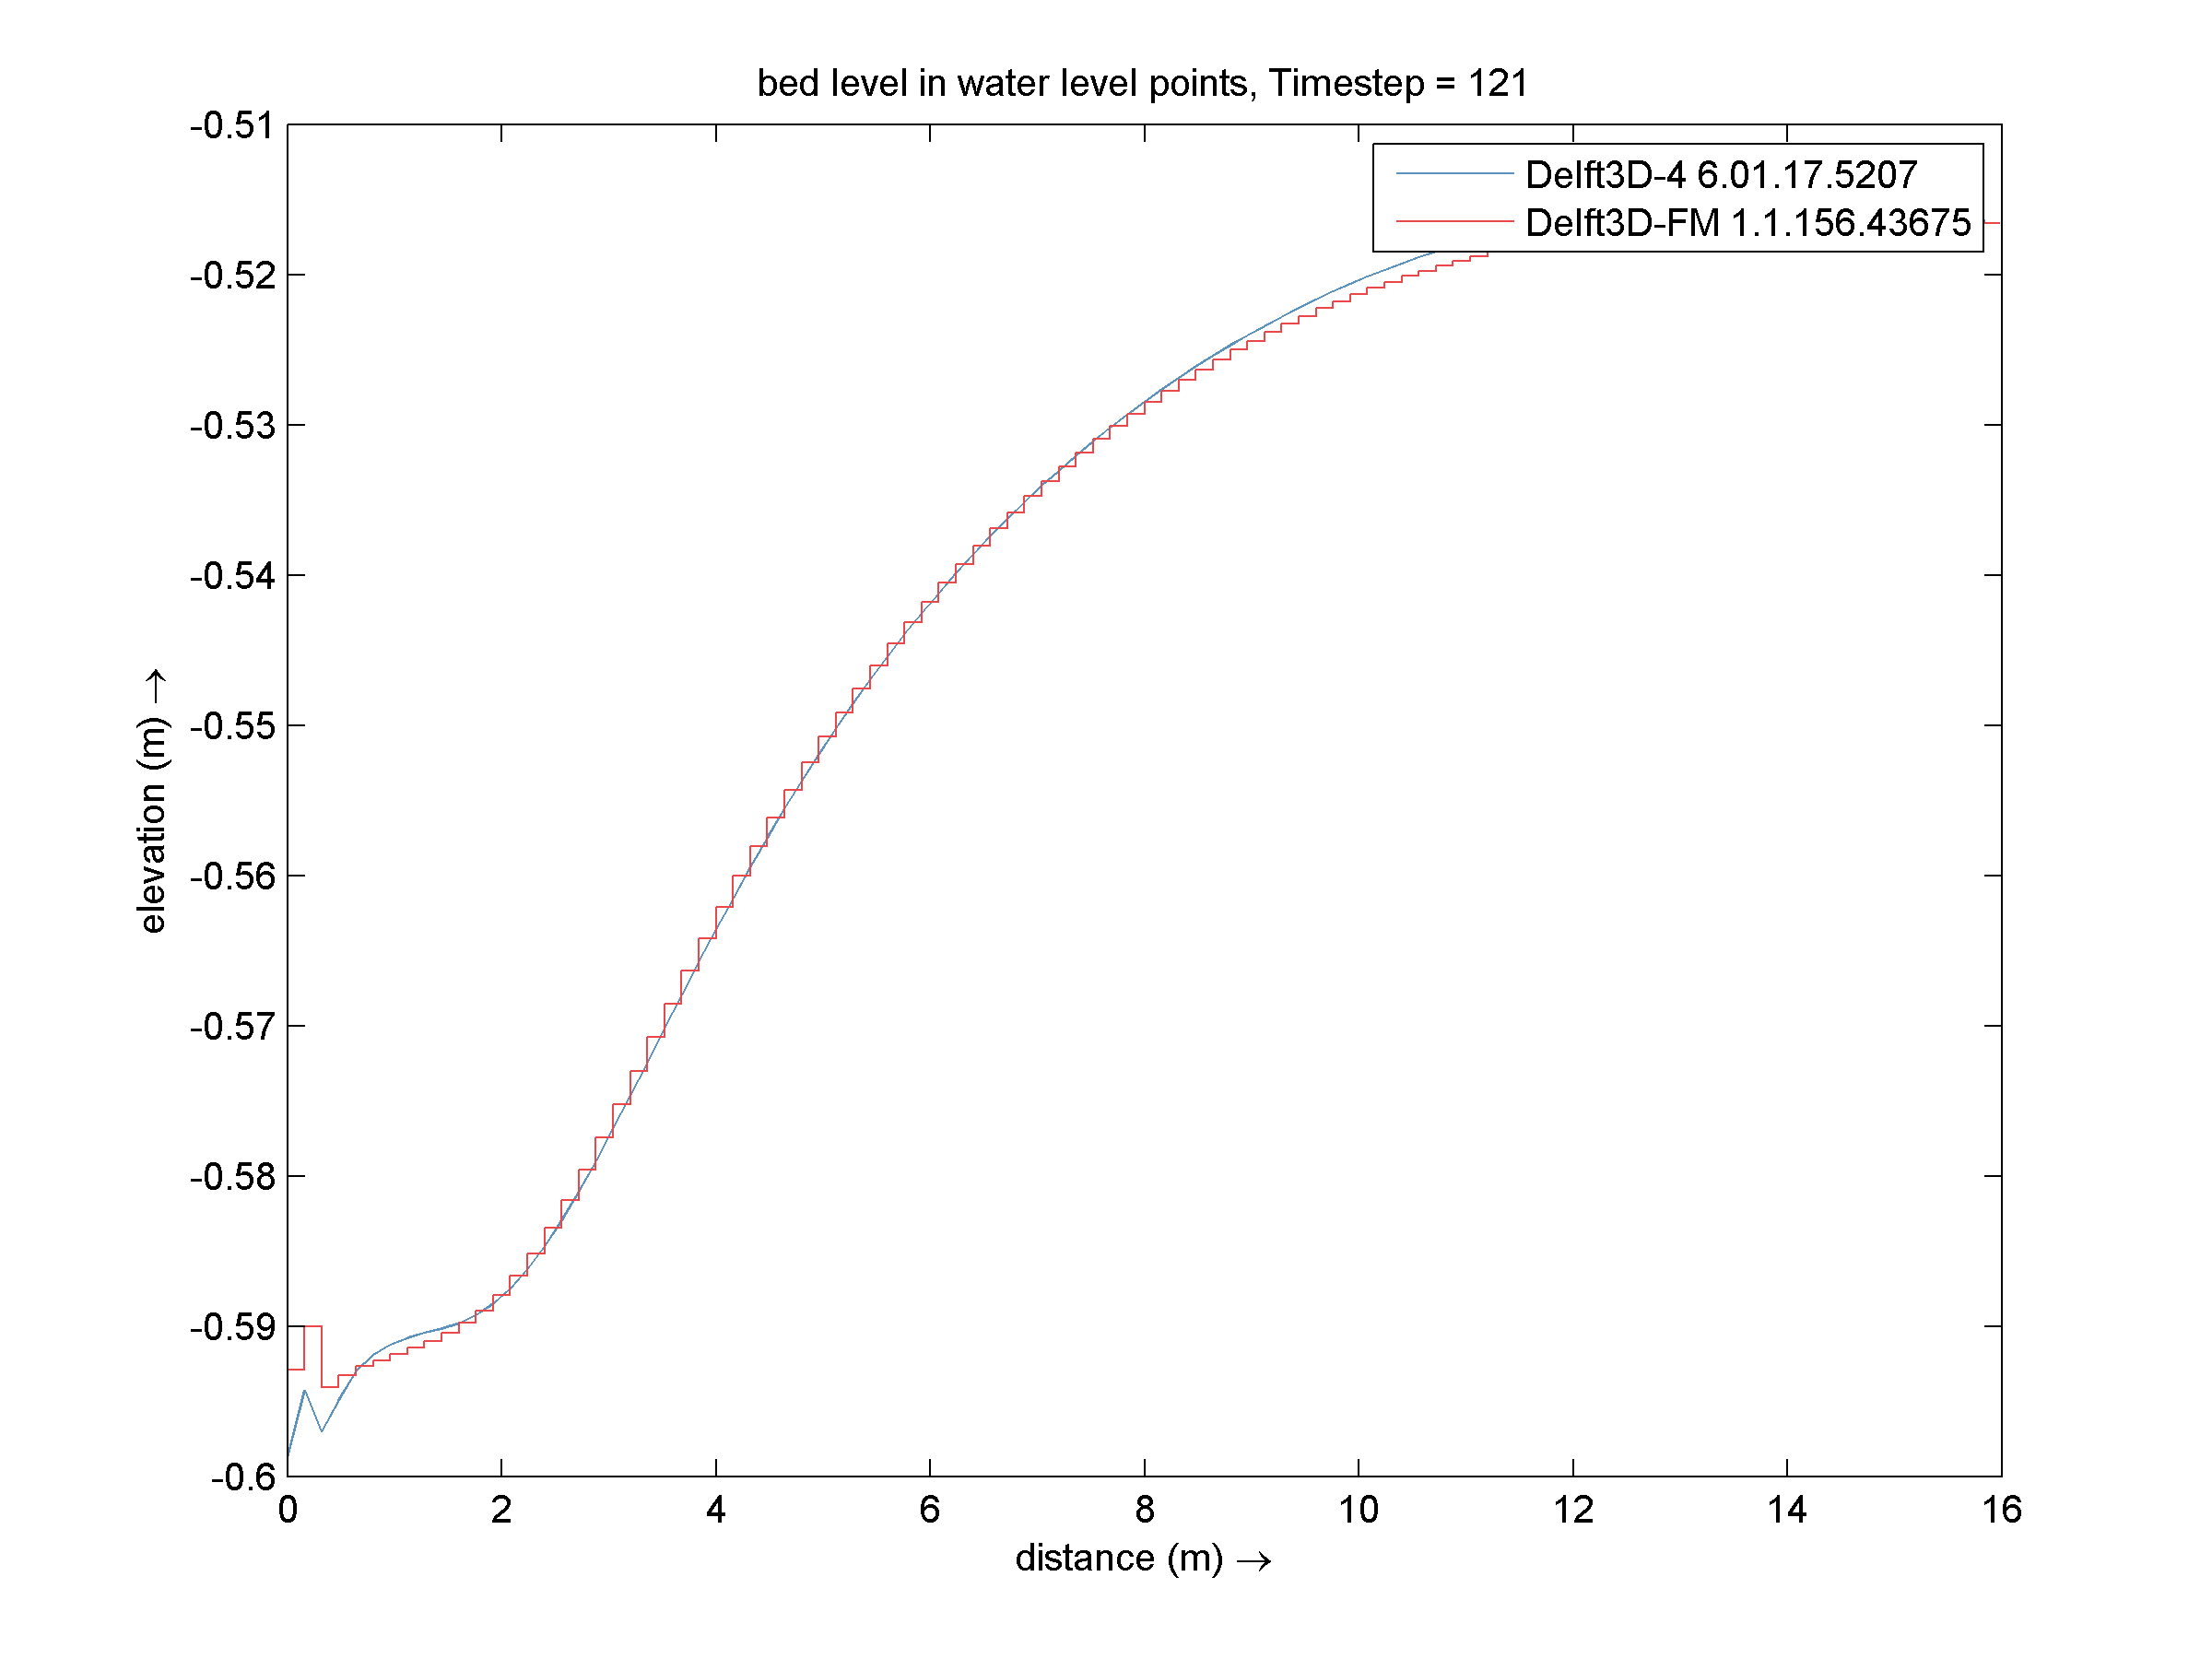
\includegraphics[width=0.70\textwidth]{figures/comparison_d3d_fm_blstr5.png}
	\end{center}
	\caption{Comparison of bed levels (same transport condition, i.e. 0.0002 m$^2$/s, for both fractions).}\label{fig:e02-fxx-cxx:bedlevelstr5}
\end{figure}

\begin{figure}[htb]
	\begin{center}
		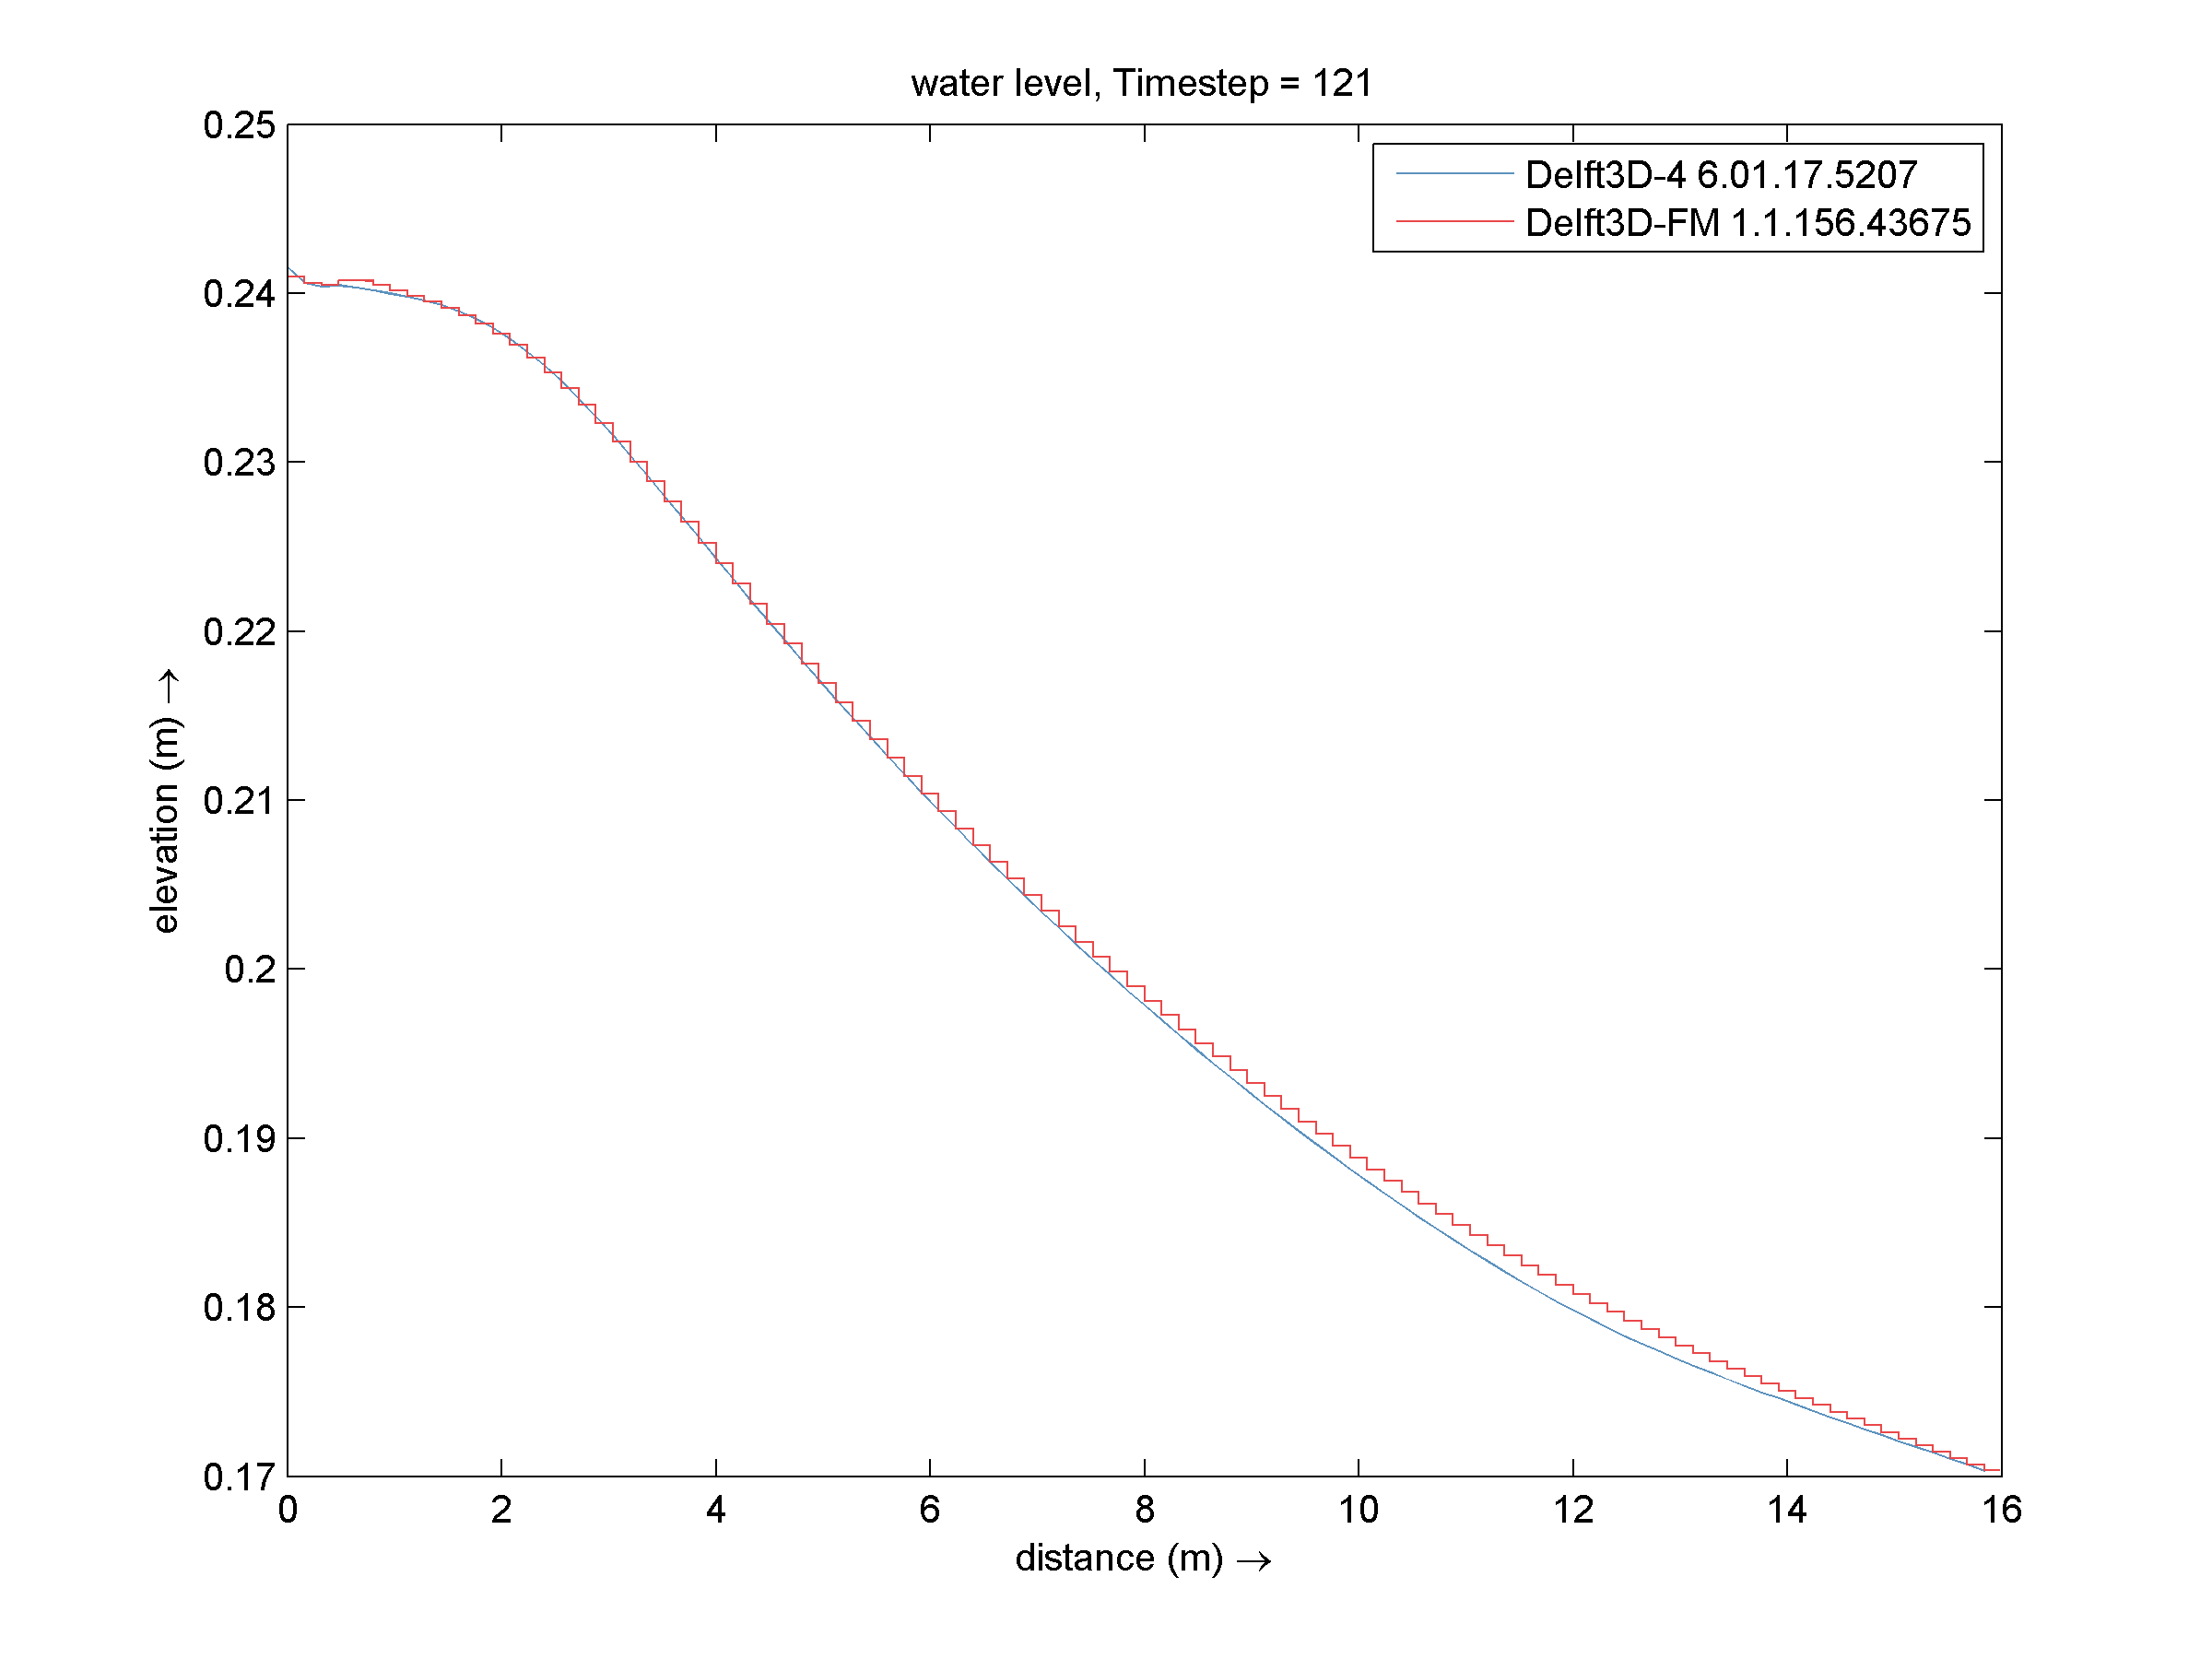
\includegraphics[width=0.70\textwidth]{figures/comparison_d3d_fm_wlstr5.png}
	\end{center}
	\caption{Comparison of water levels (same transport condition, i.e. 0.0002 m$^2$/s, for both fractions).}\label{fig:e02-fxx-cxx:waterlevelstr5}
\end{figure}

\begin{figure}[htb]
	\begin{center}
		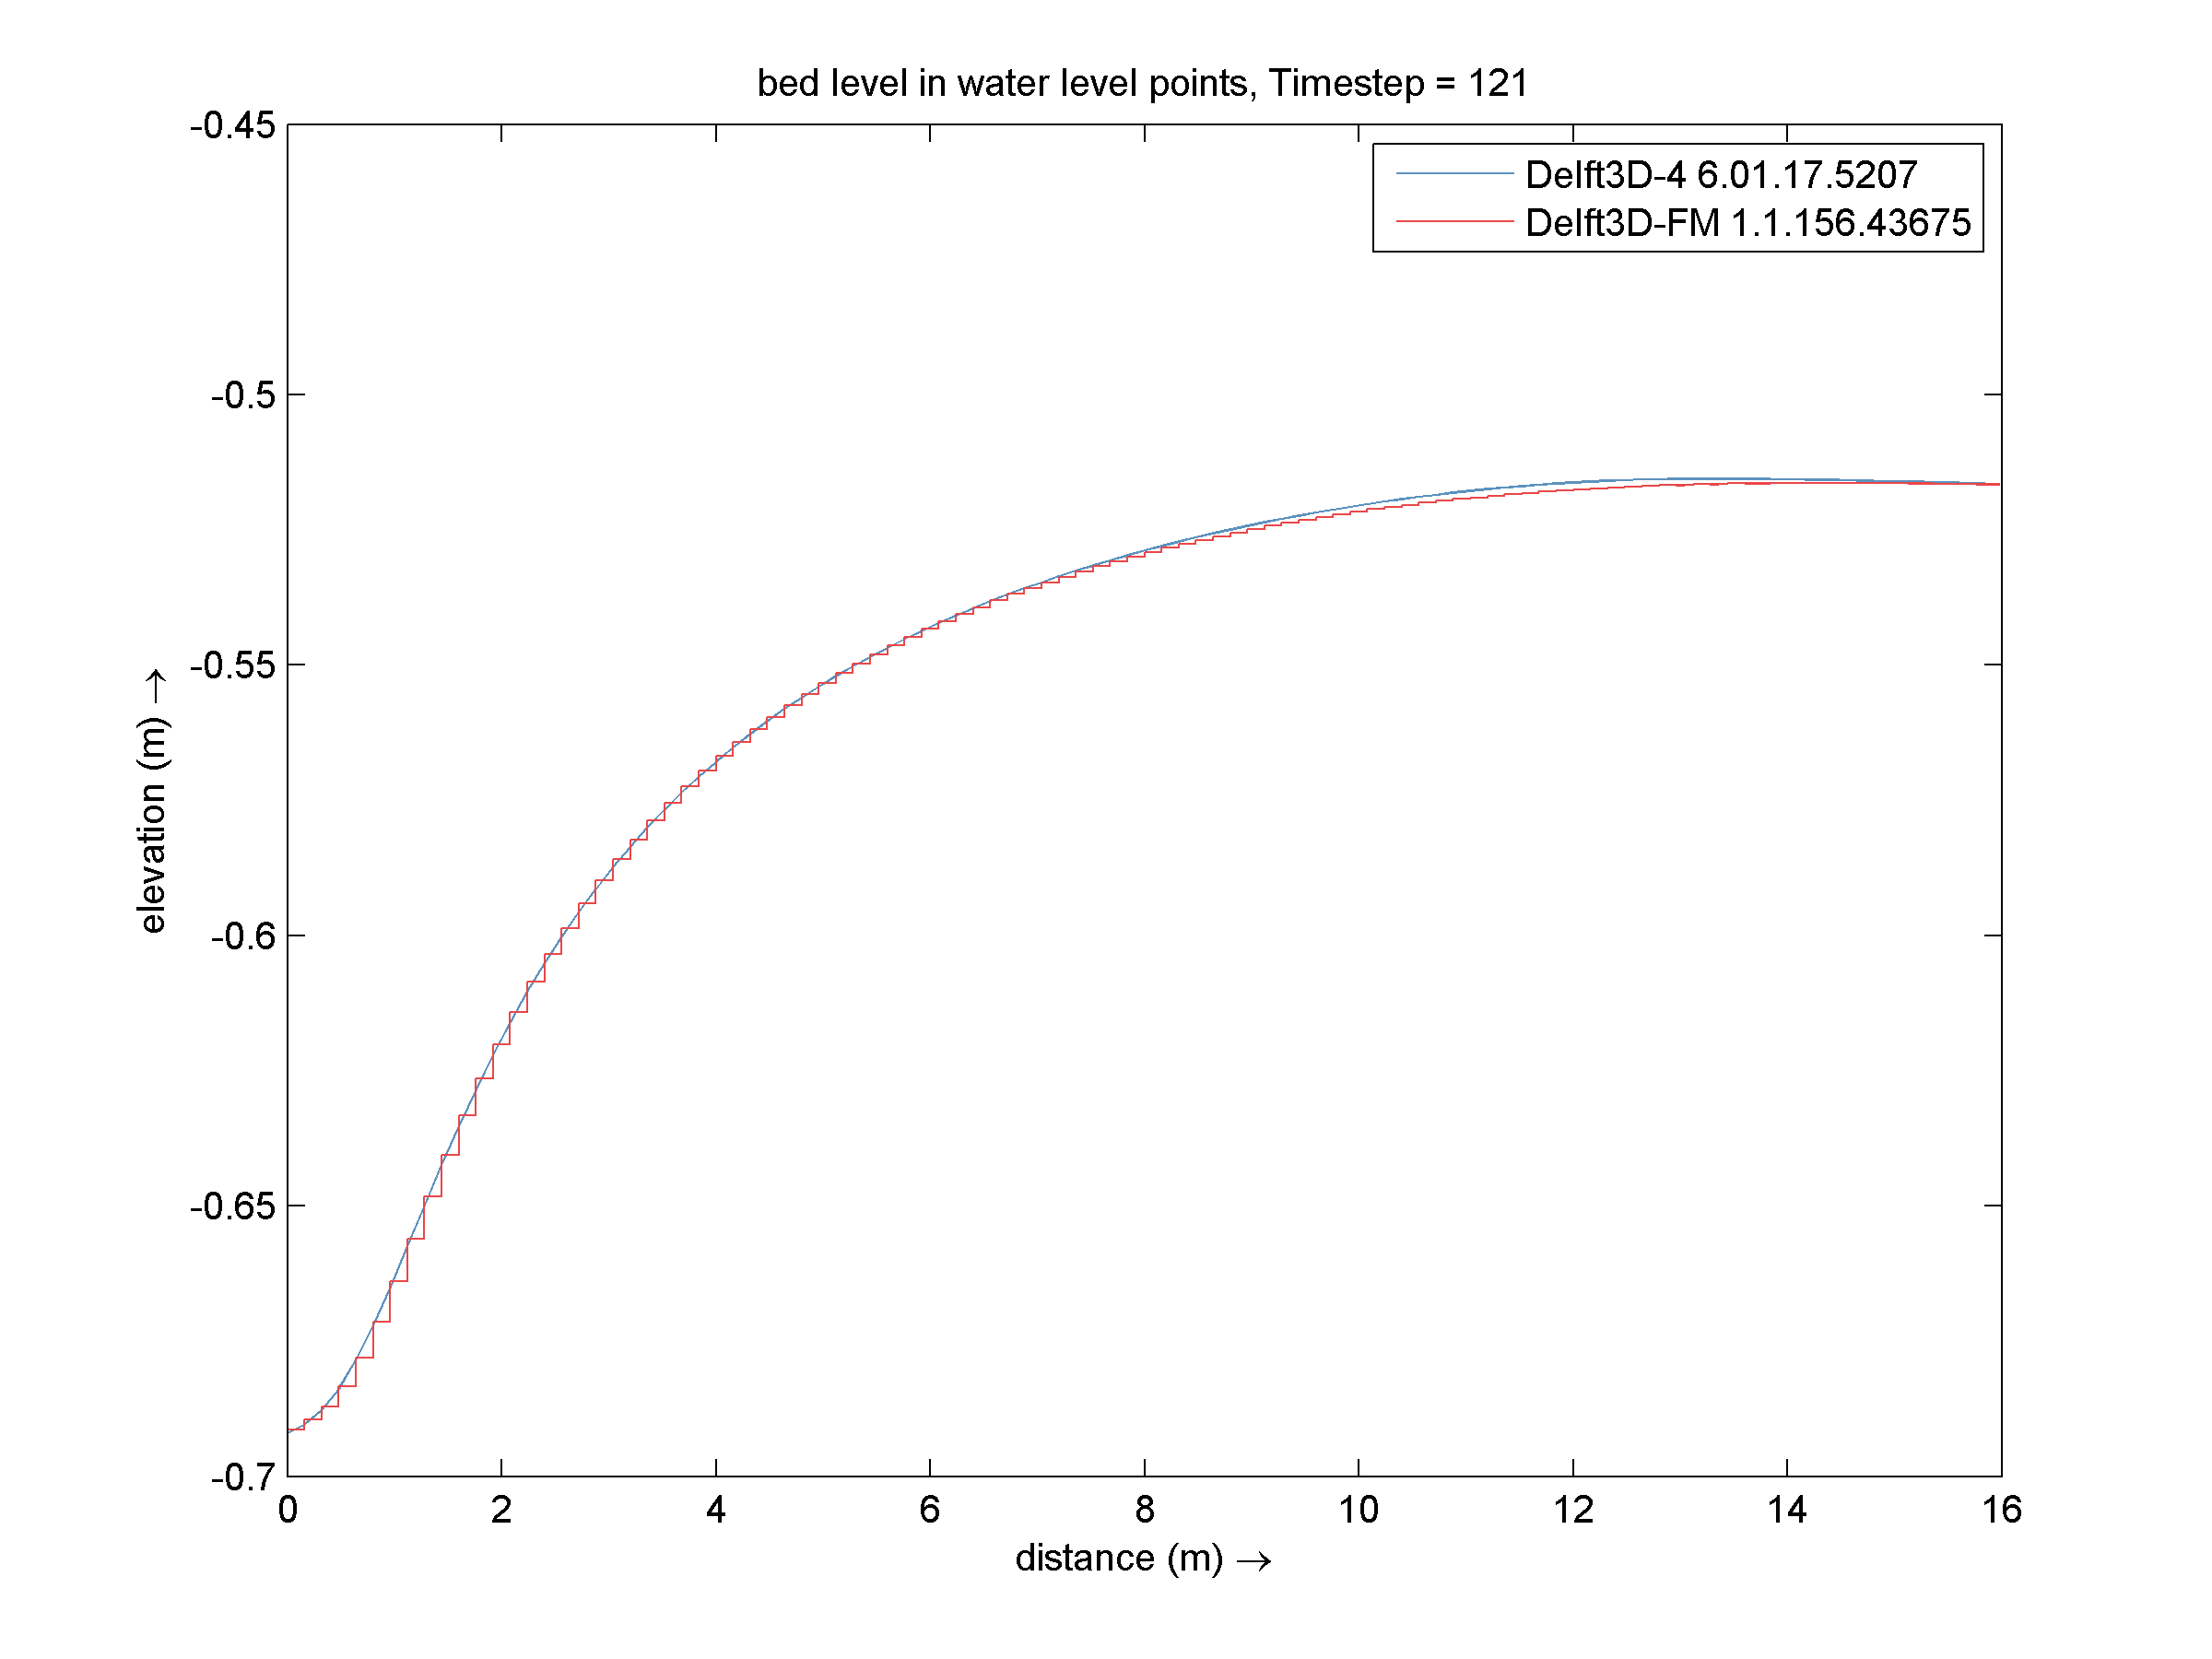
\includegraphics[width=0.70\textwidth]{figures/comparison_d3d_fm_blstr6.png}
	\end{center}
	\caption{Comparison of bed levels (transport condition with 0.0002 m$^2$/s and 0 m$^2$/s for fractions 1 and 2 respectively).}\label{fig:e02-fxx-cxx:bedlevelstr6}
\end{figure}

\begin{figure}[htb]
	\begin{center}
		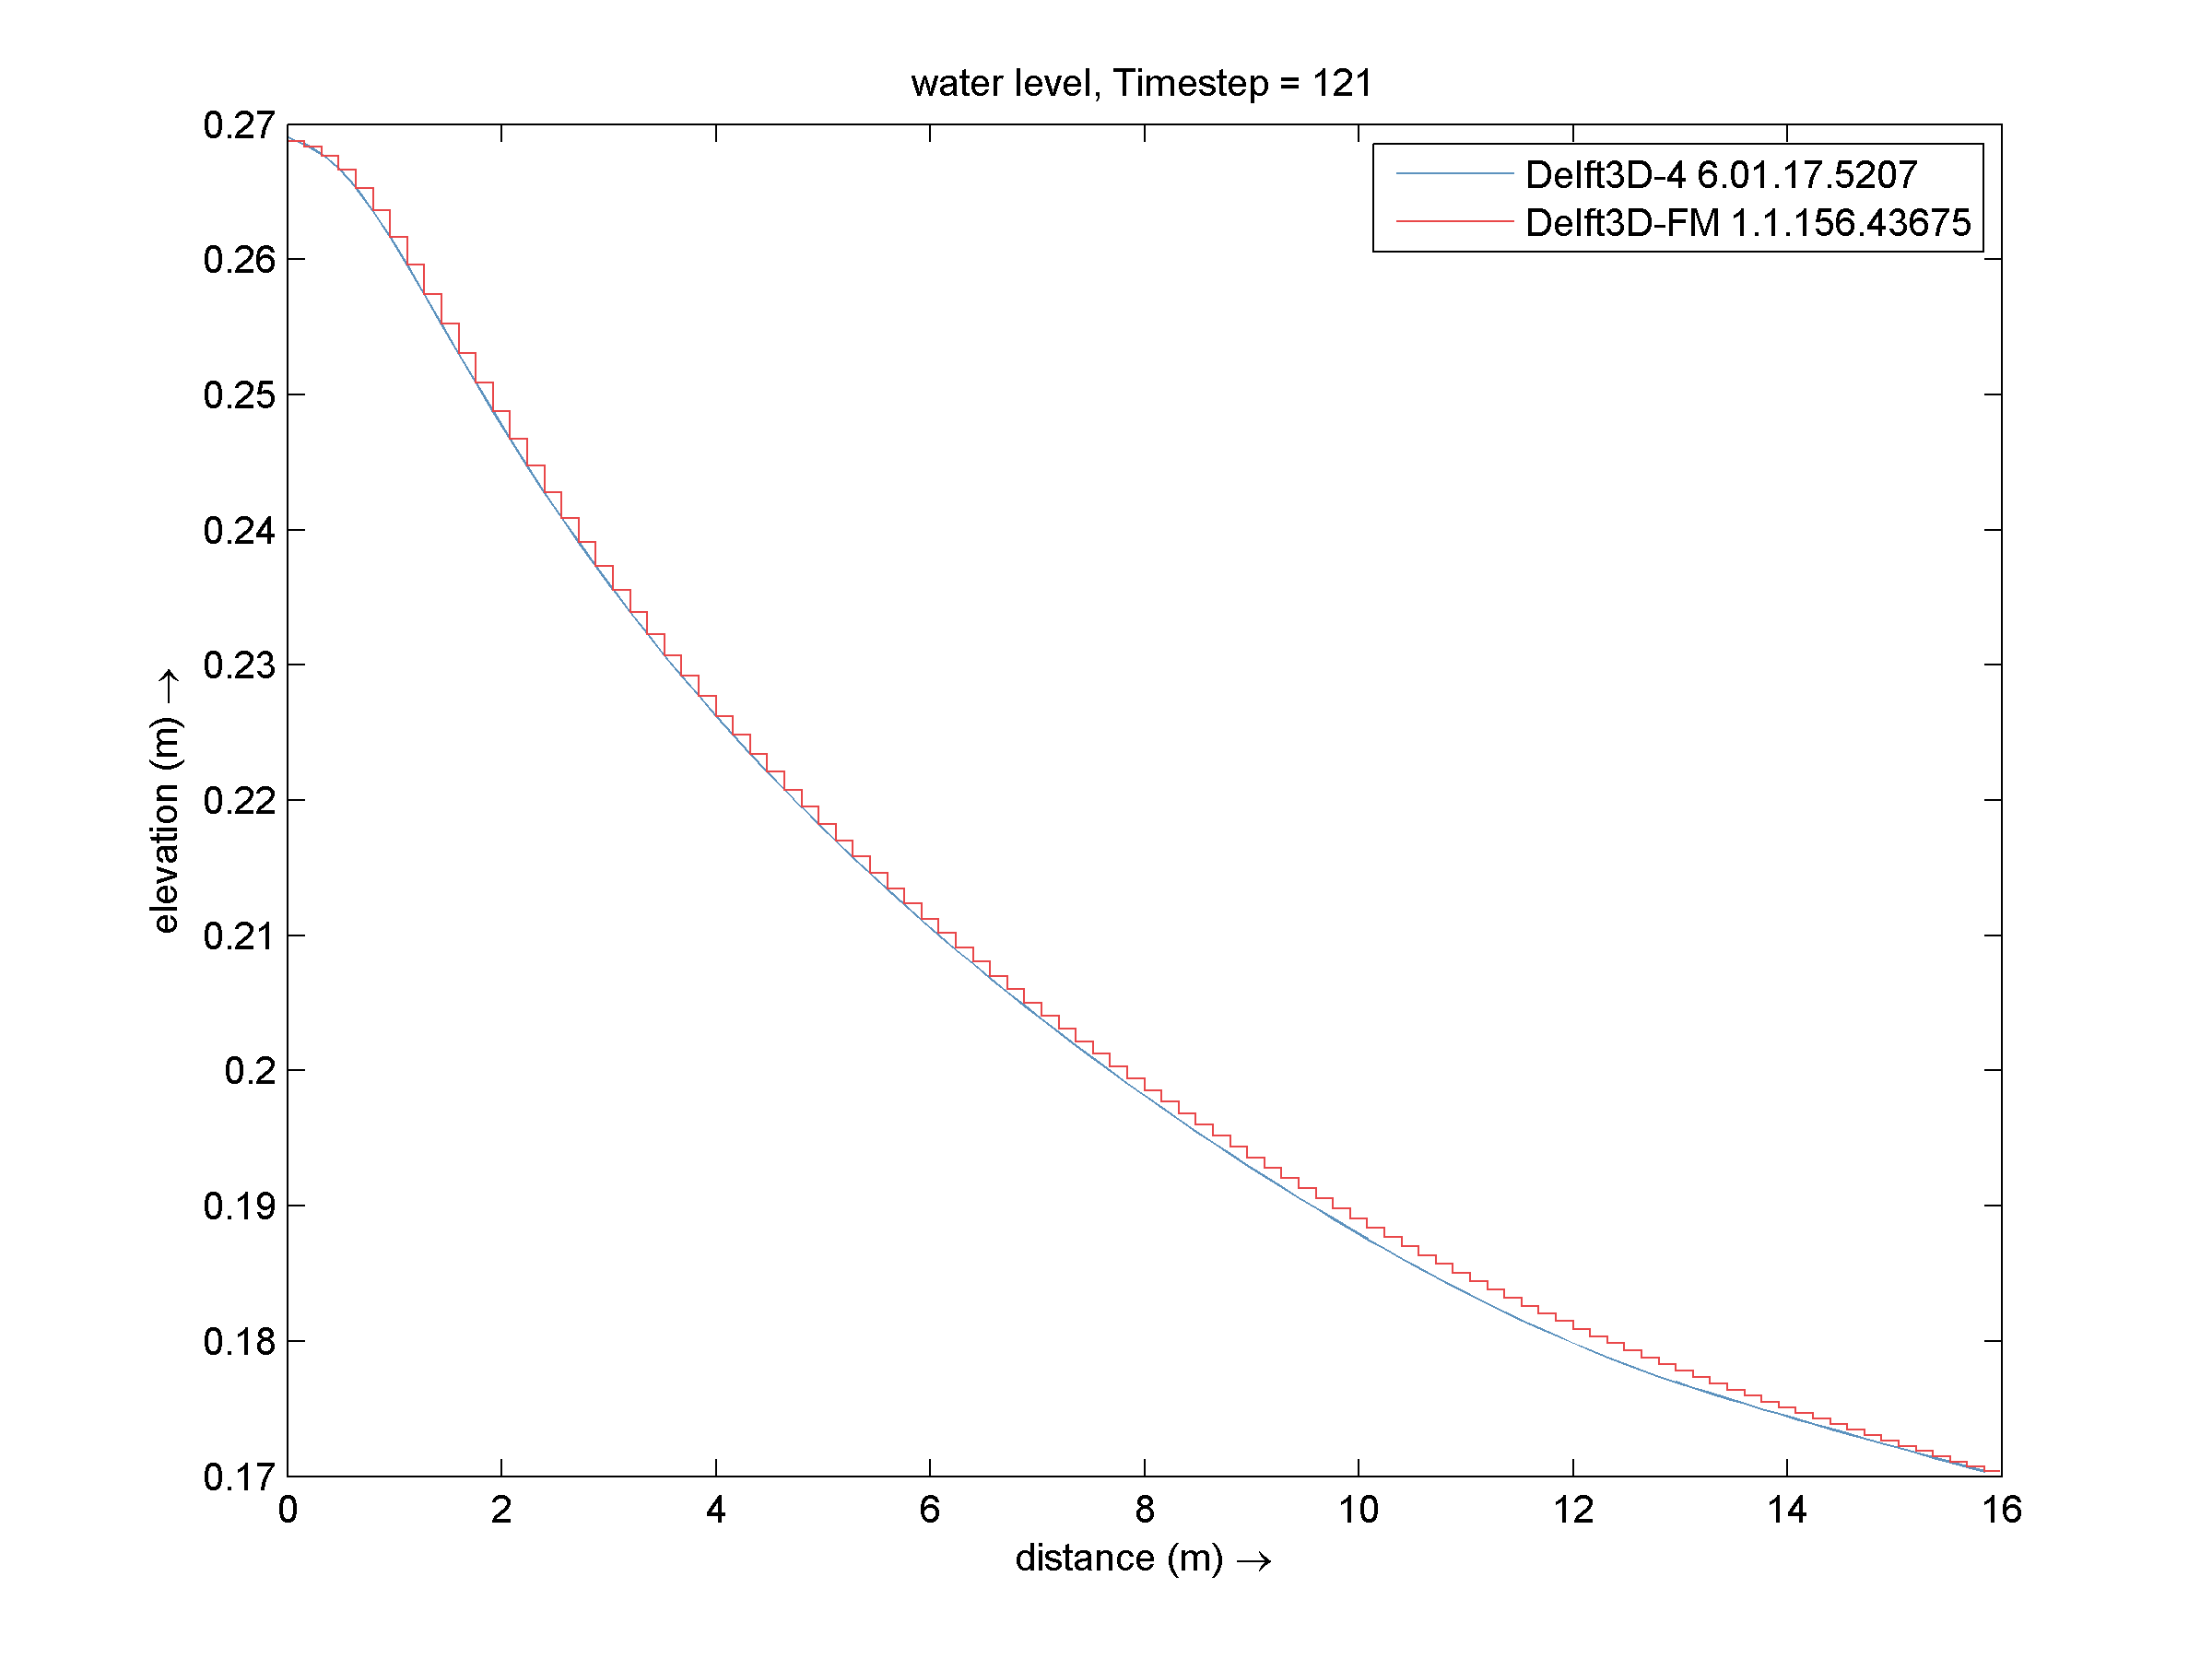
\includegraphics[width=0.70\textwidth]{figures/comparison_d3d_fm_wlstr6.png}
	\end{center}
	\caption{Comparison of water levels (transport condition with 0.0002 m$^2$/s and 0 m$^2$/s for fractions 1 and 2 respectively).}\label{fig:e02-fxx-cxx:waterlevelstr6}
\end{figure}

\begin{figure}[htb]
	\begin{center}
		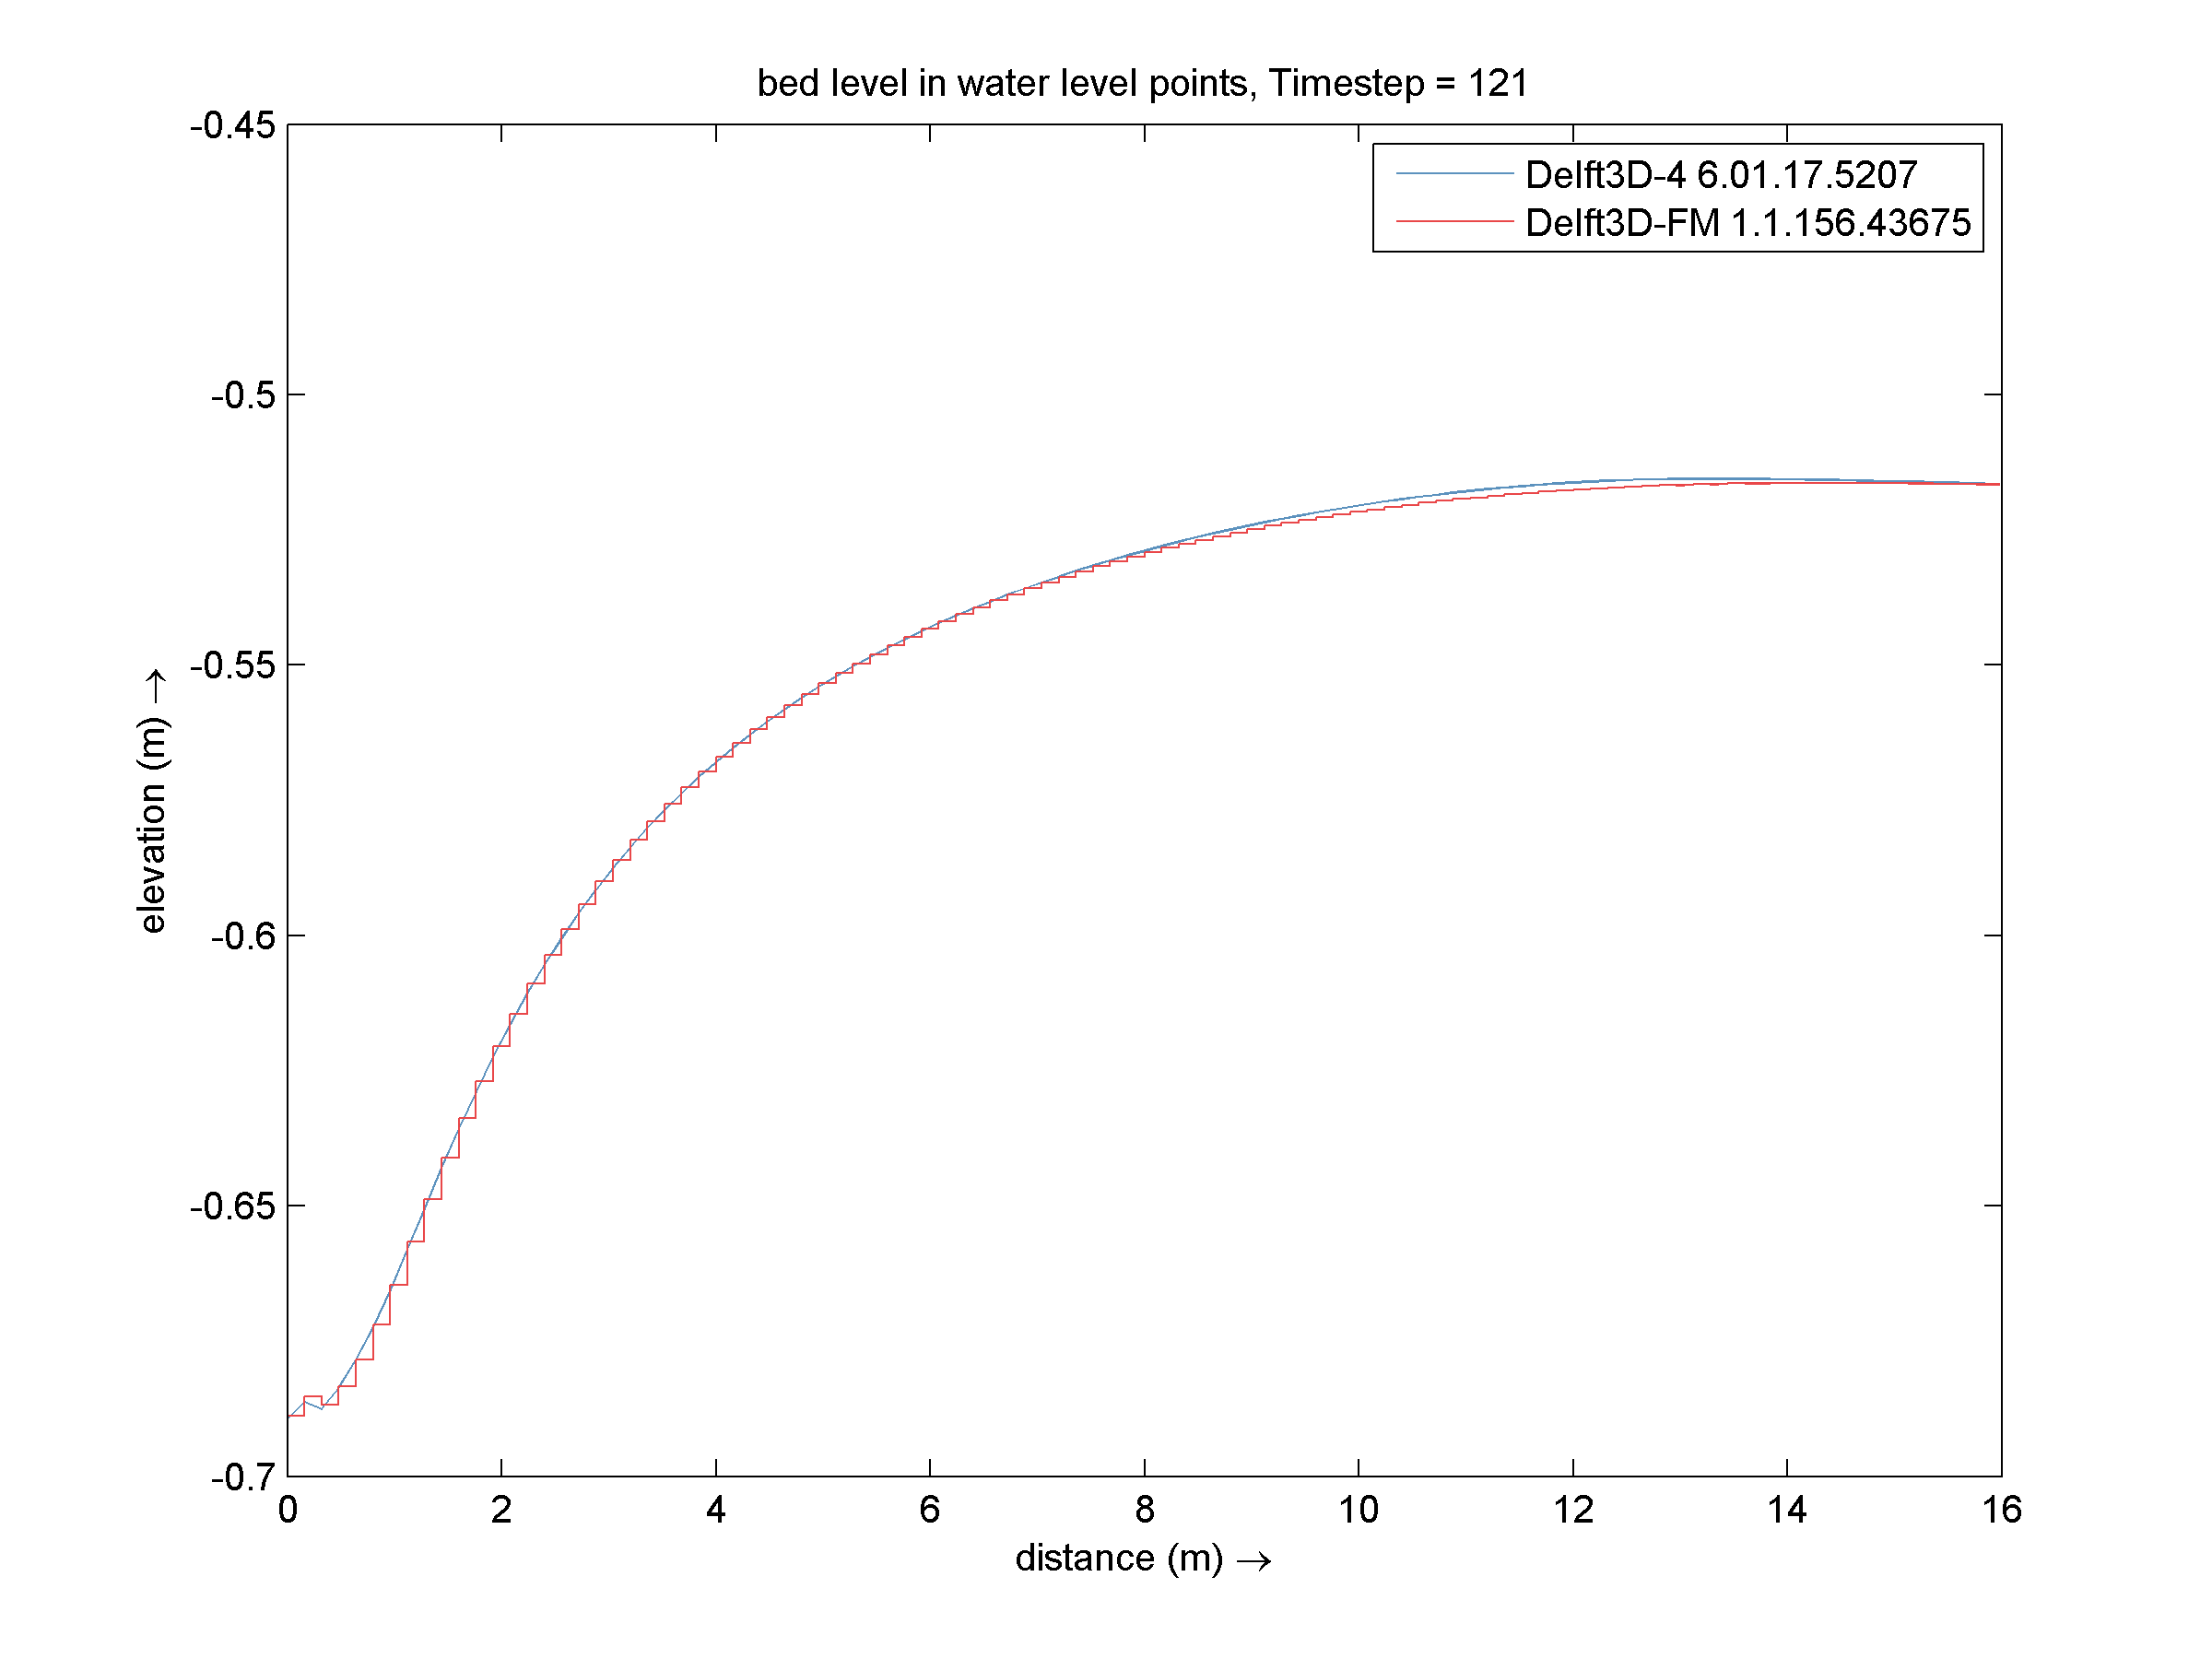
\includegraphics[width=0.70\textwidth]{figures/comparison_d3d_fm_blstr7.png}
	\end{center}
	\caption{Comparison of bed levels (transport condition with 0 m$^2$/s and 0.0002 m$^2$/s for fractions 1 and 2 respectively).}\label{fig:e02-fxx-cxx:bedlevelstr7}
\end{figure}

\begin{figure}[htb]
	\begin{center}
		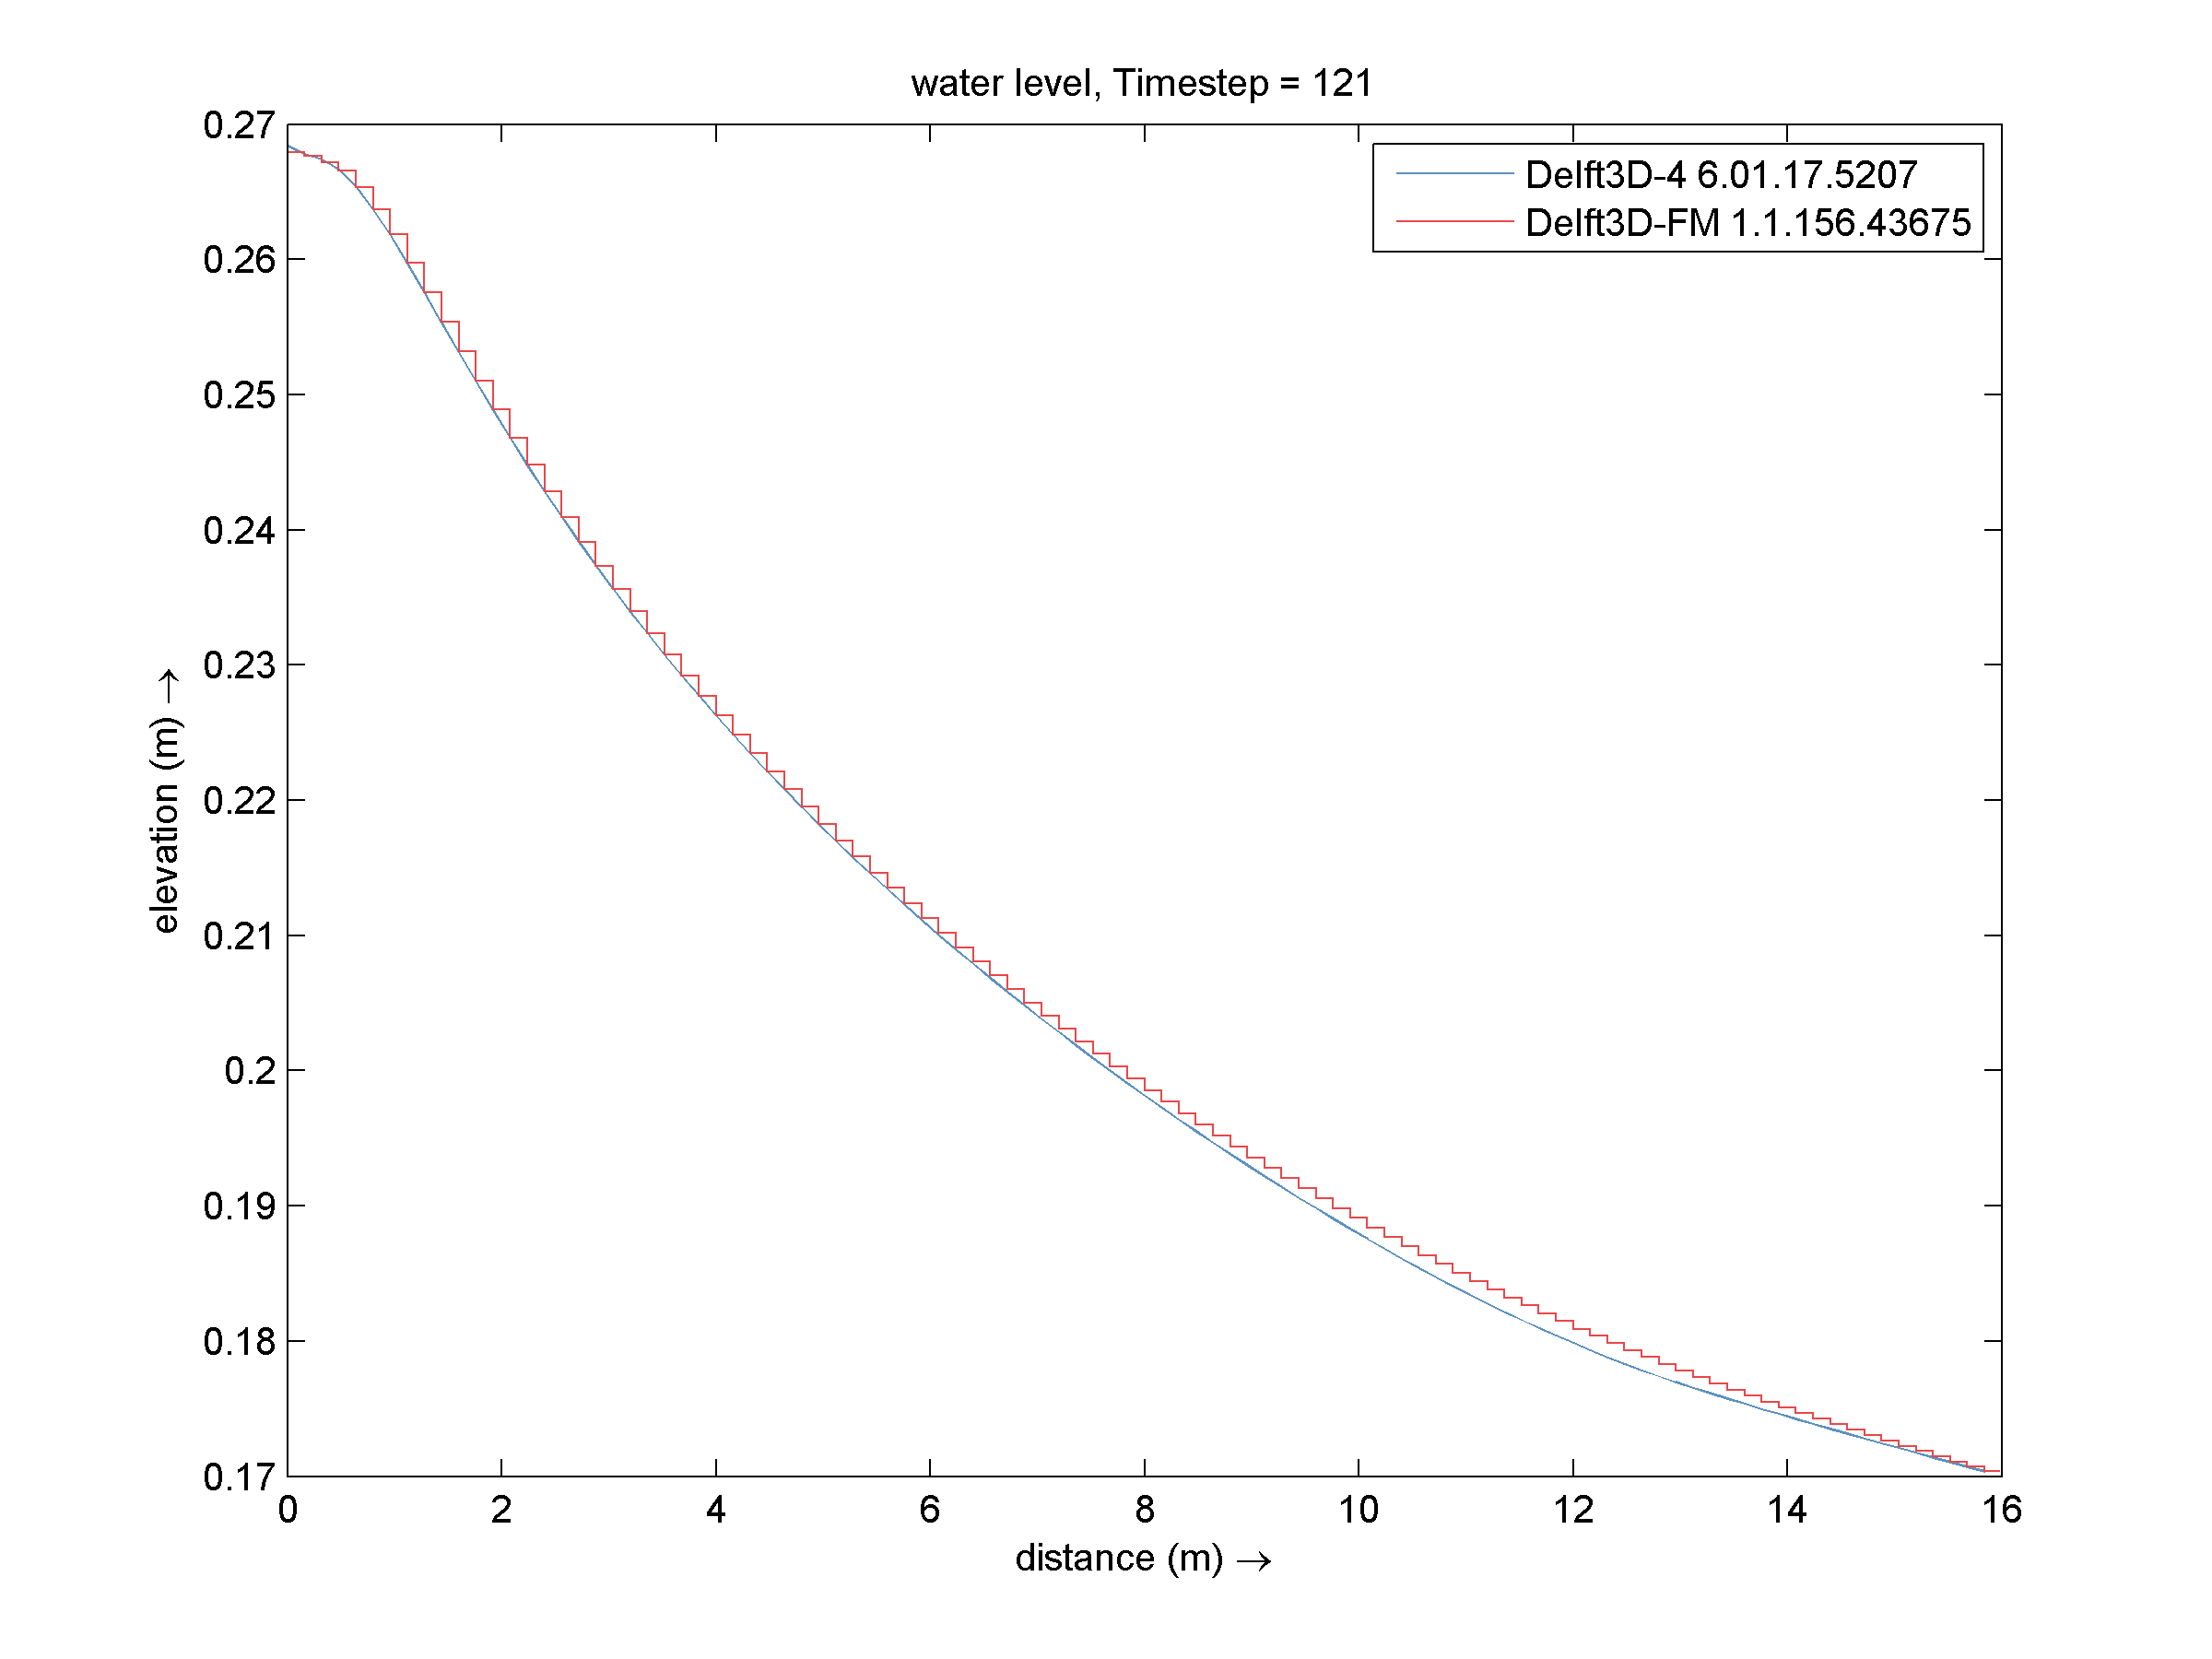
\includegraphics[width=0.70\textwidth]{figures/comparison_d3d_fm_wlstr7.png}
	\end{center}
	\caption{Comparison of water levels (transport condition with 0 m$^2$/s and 0.0002 m$^2$/s for fractions 1 and 2 respectively).}\label{fig:e02-fxx-cxx:waterlevelstr7}
\end{figure}

\begin{figure}[htb]
	\begin{center}
		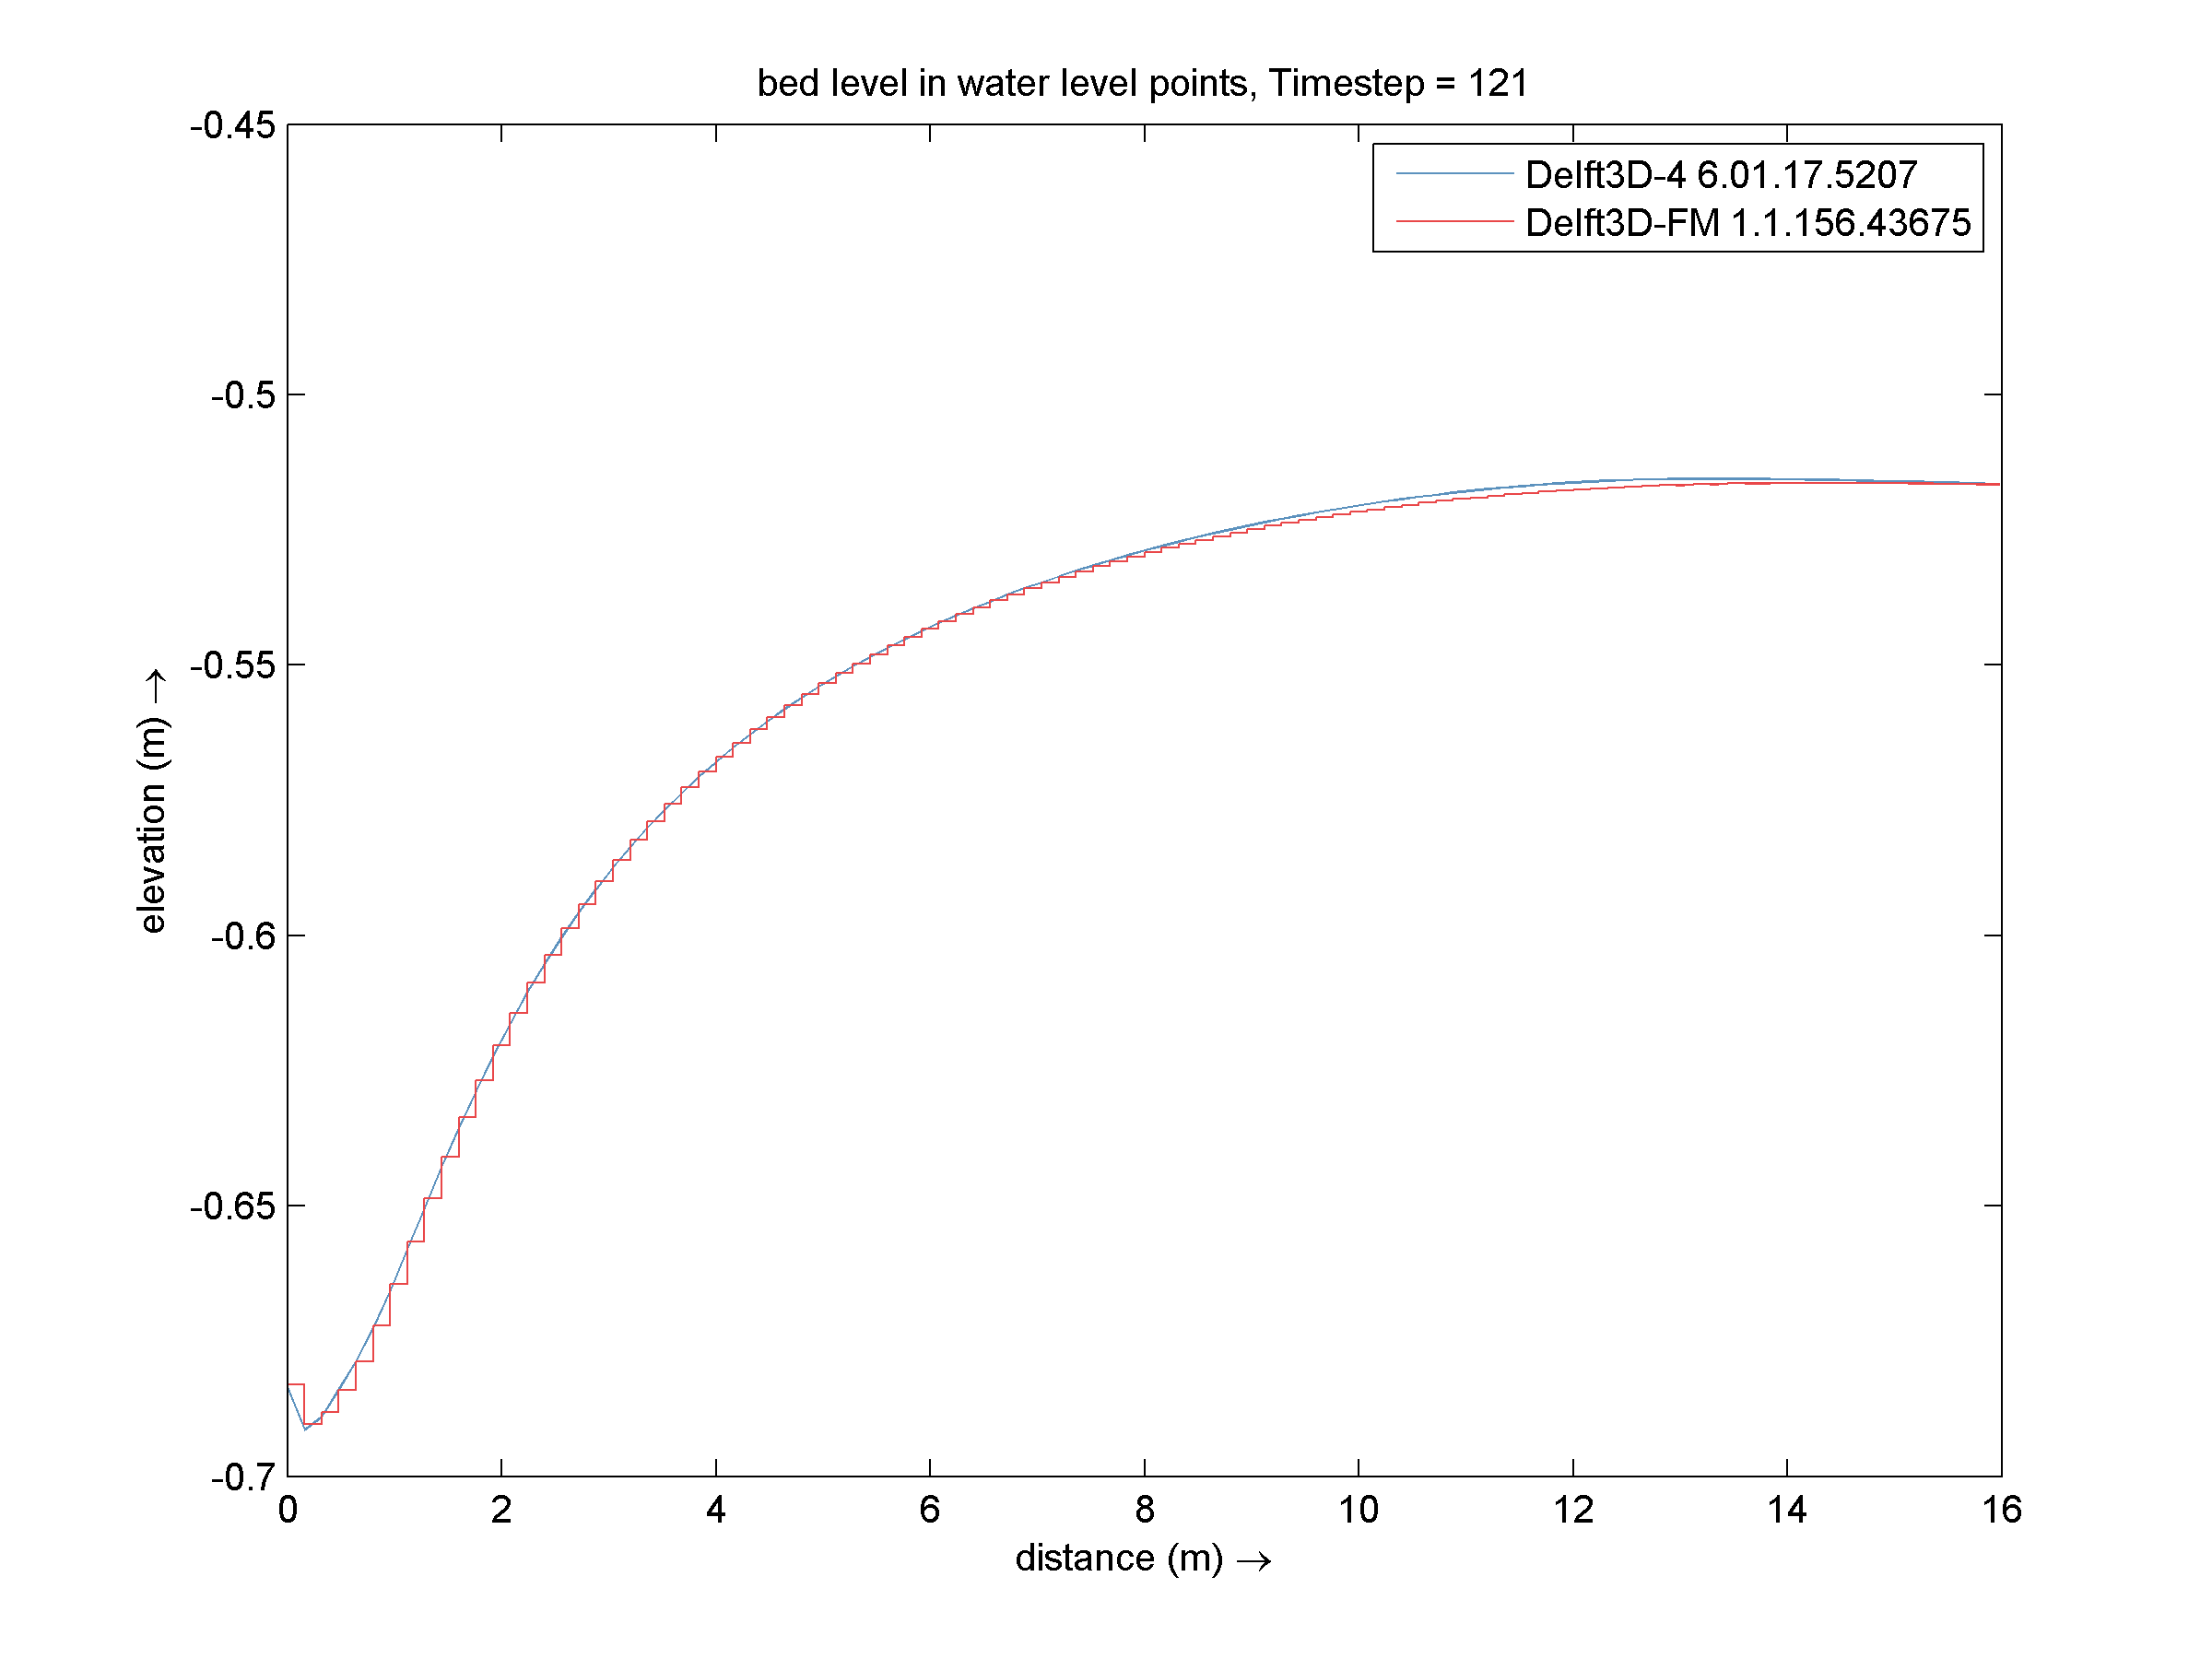
\includegraphics[width=0.70\textwidth]{figures/comparison_d3d_fm_blstr8.png}
	\end{center}
	\caption{Comparison of bed levels (transport condition with 0.0001 m$^2$/s and 0.0001 m$^2$/s for fractions 1 and 2 respectively).}\label{fig:e02-fxx-cxx:bedlevelstr8}
\end{figure}

\begin{figure}[htb]
	\begin{center}
		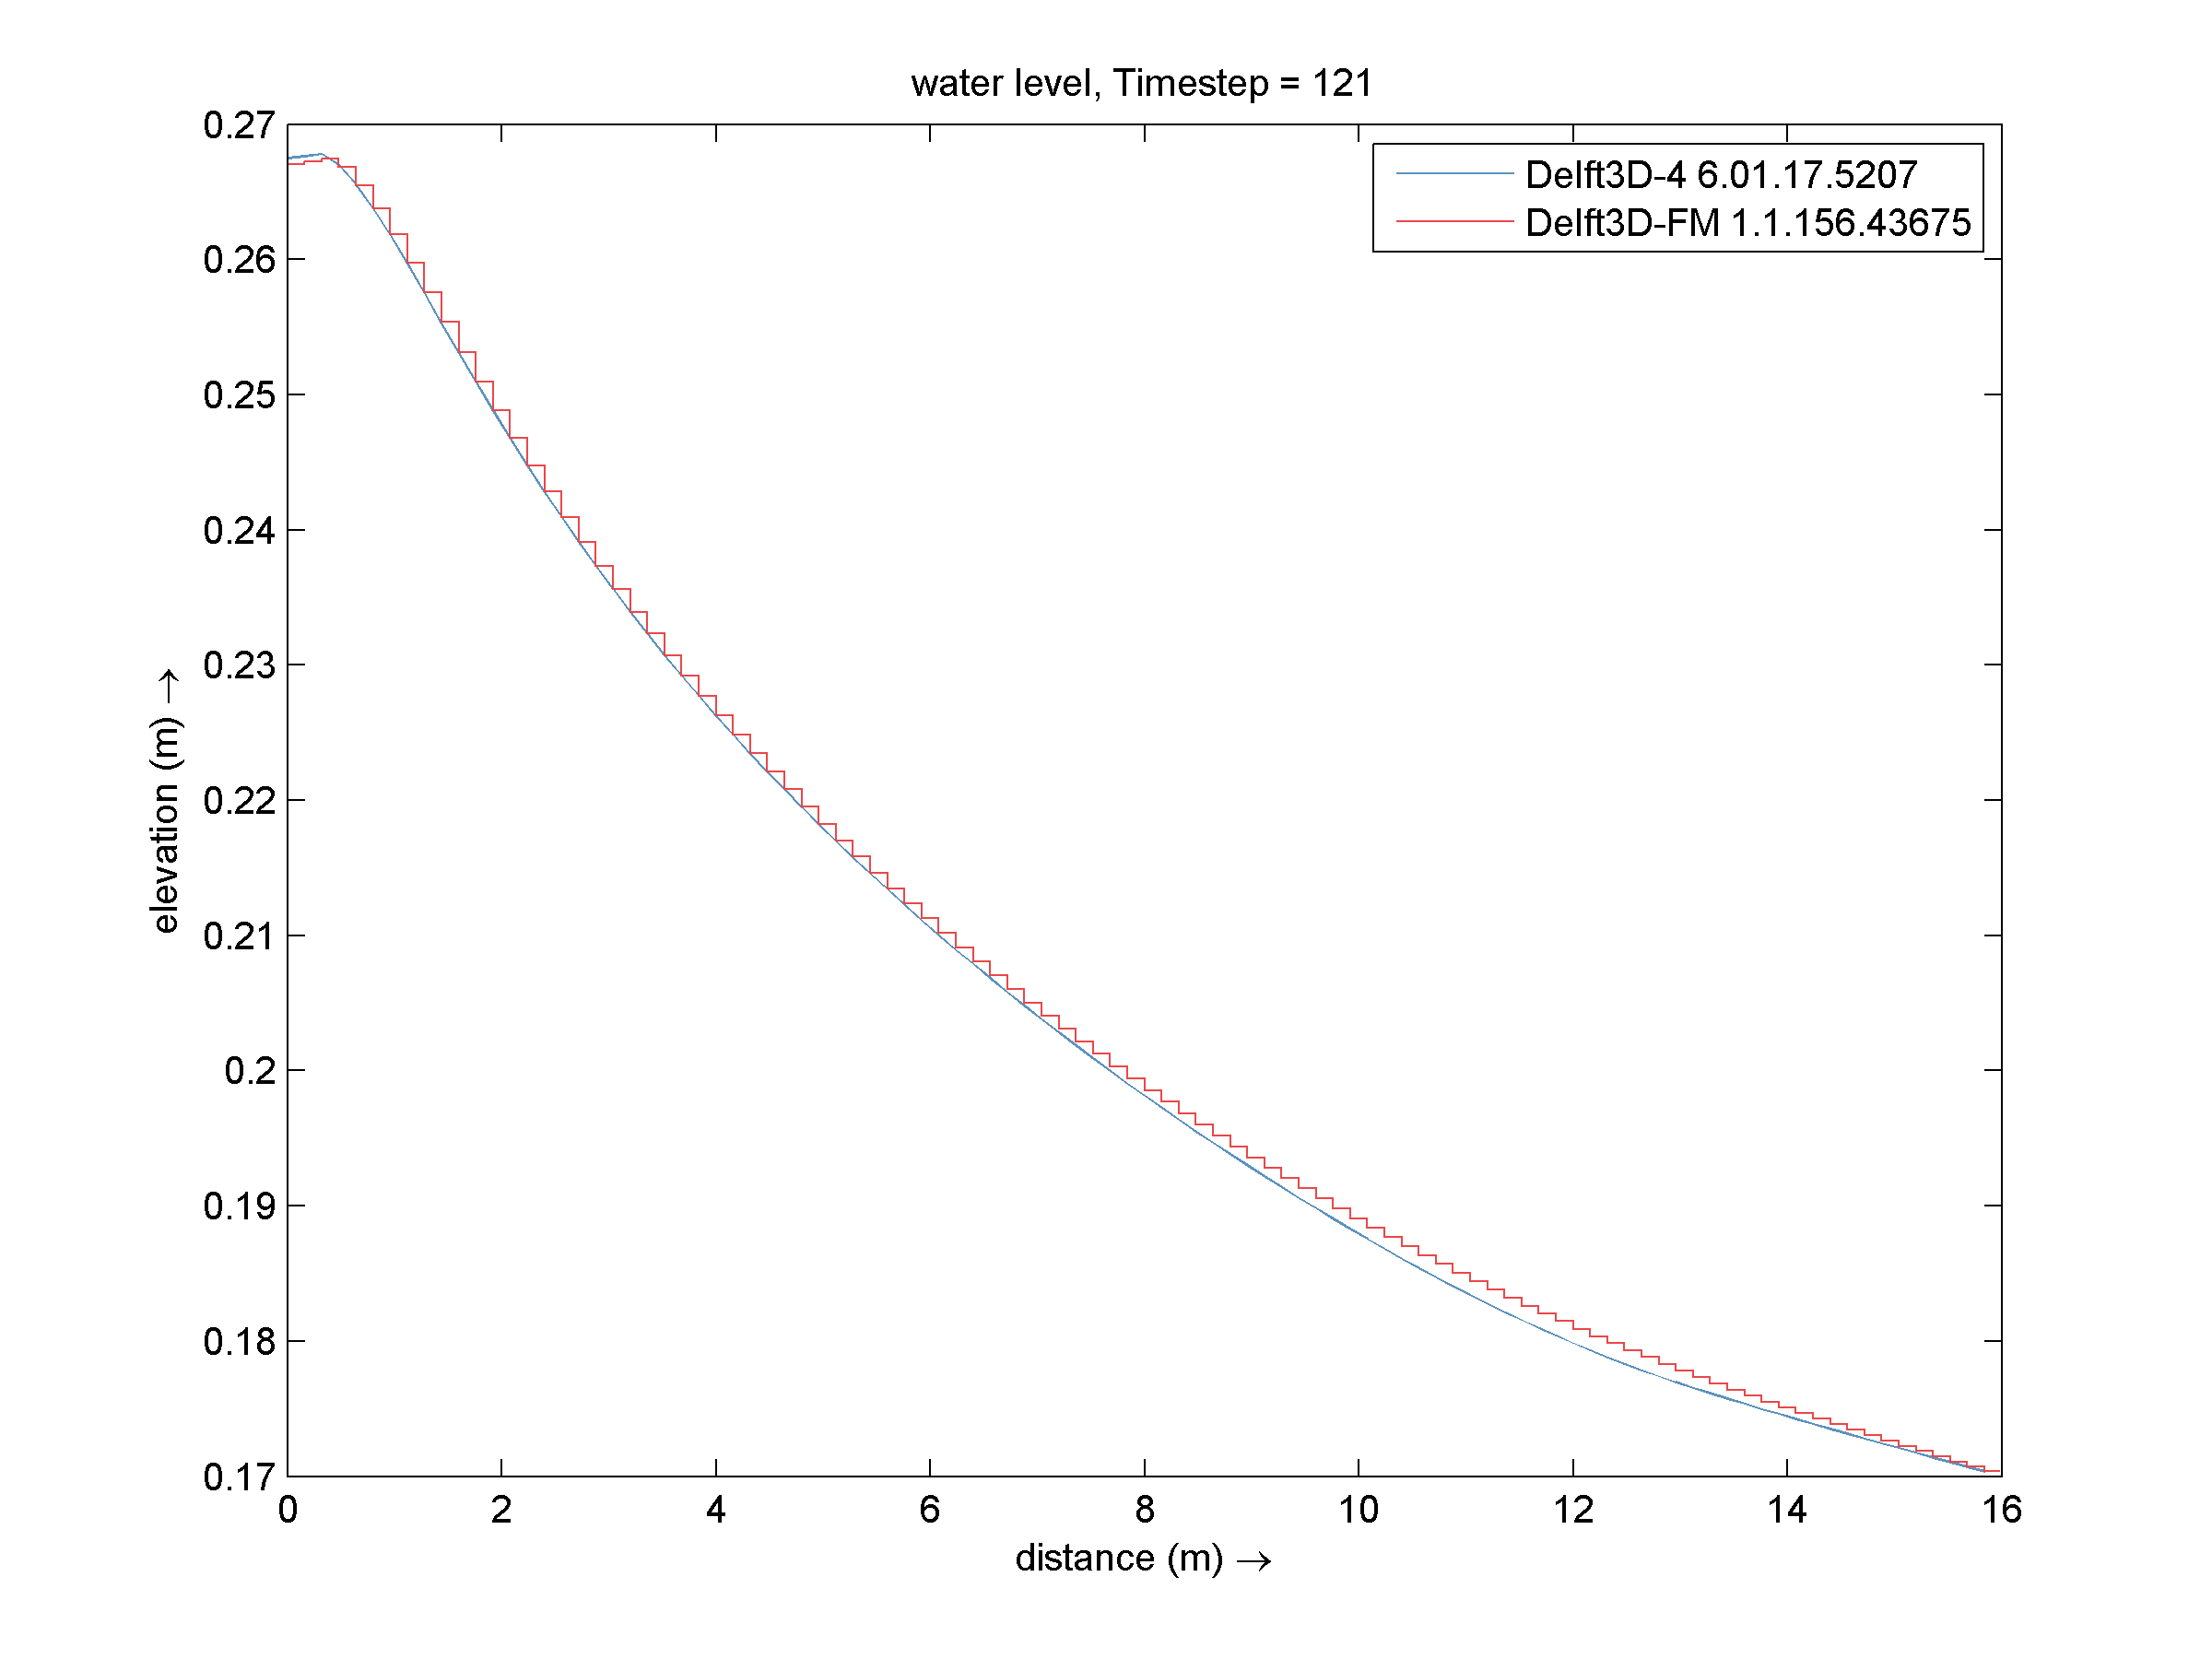
\includegraphics[width=0.70\textwidth]{figures/comparison_d3d_fm_wlstr8.png}
	\end{center}
	\caption{Comparison of water levels (transport condition with 0.0001 m$^2$/s and 0.0001 m$^2$/s for fractions 1 and 2 respectively).}\label{fig:e02-fxx-cxx:waterlevelstr8}
\end{figure}

\newpage

\begin{figure}[htb]
	\begin{center}
		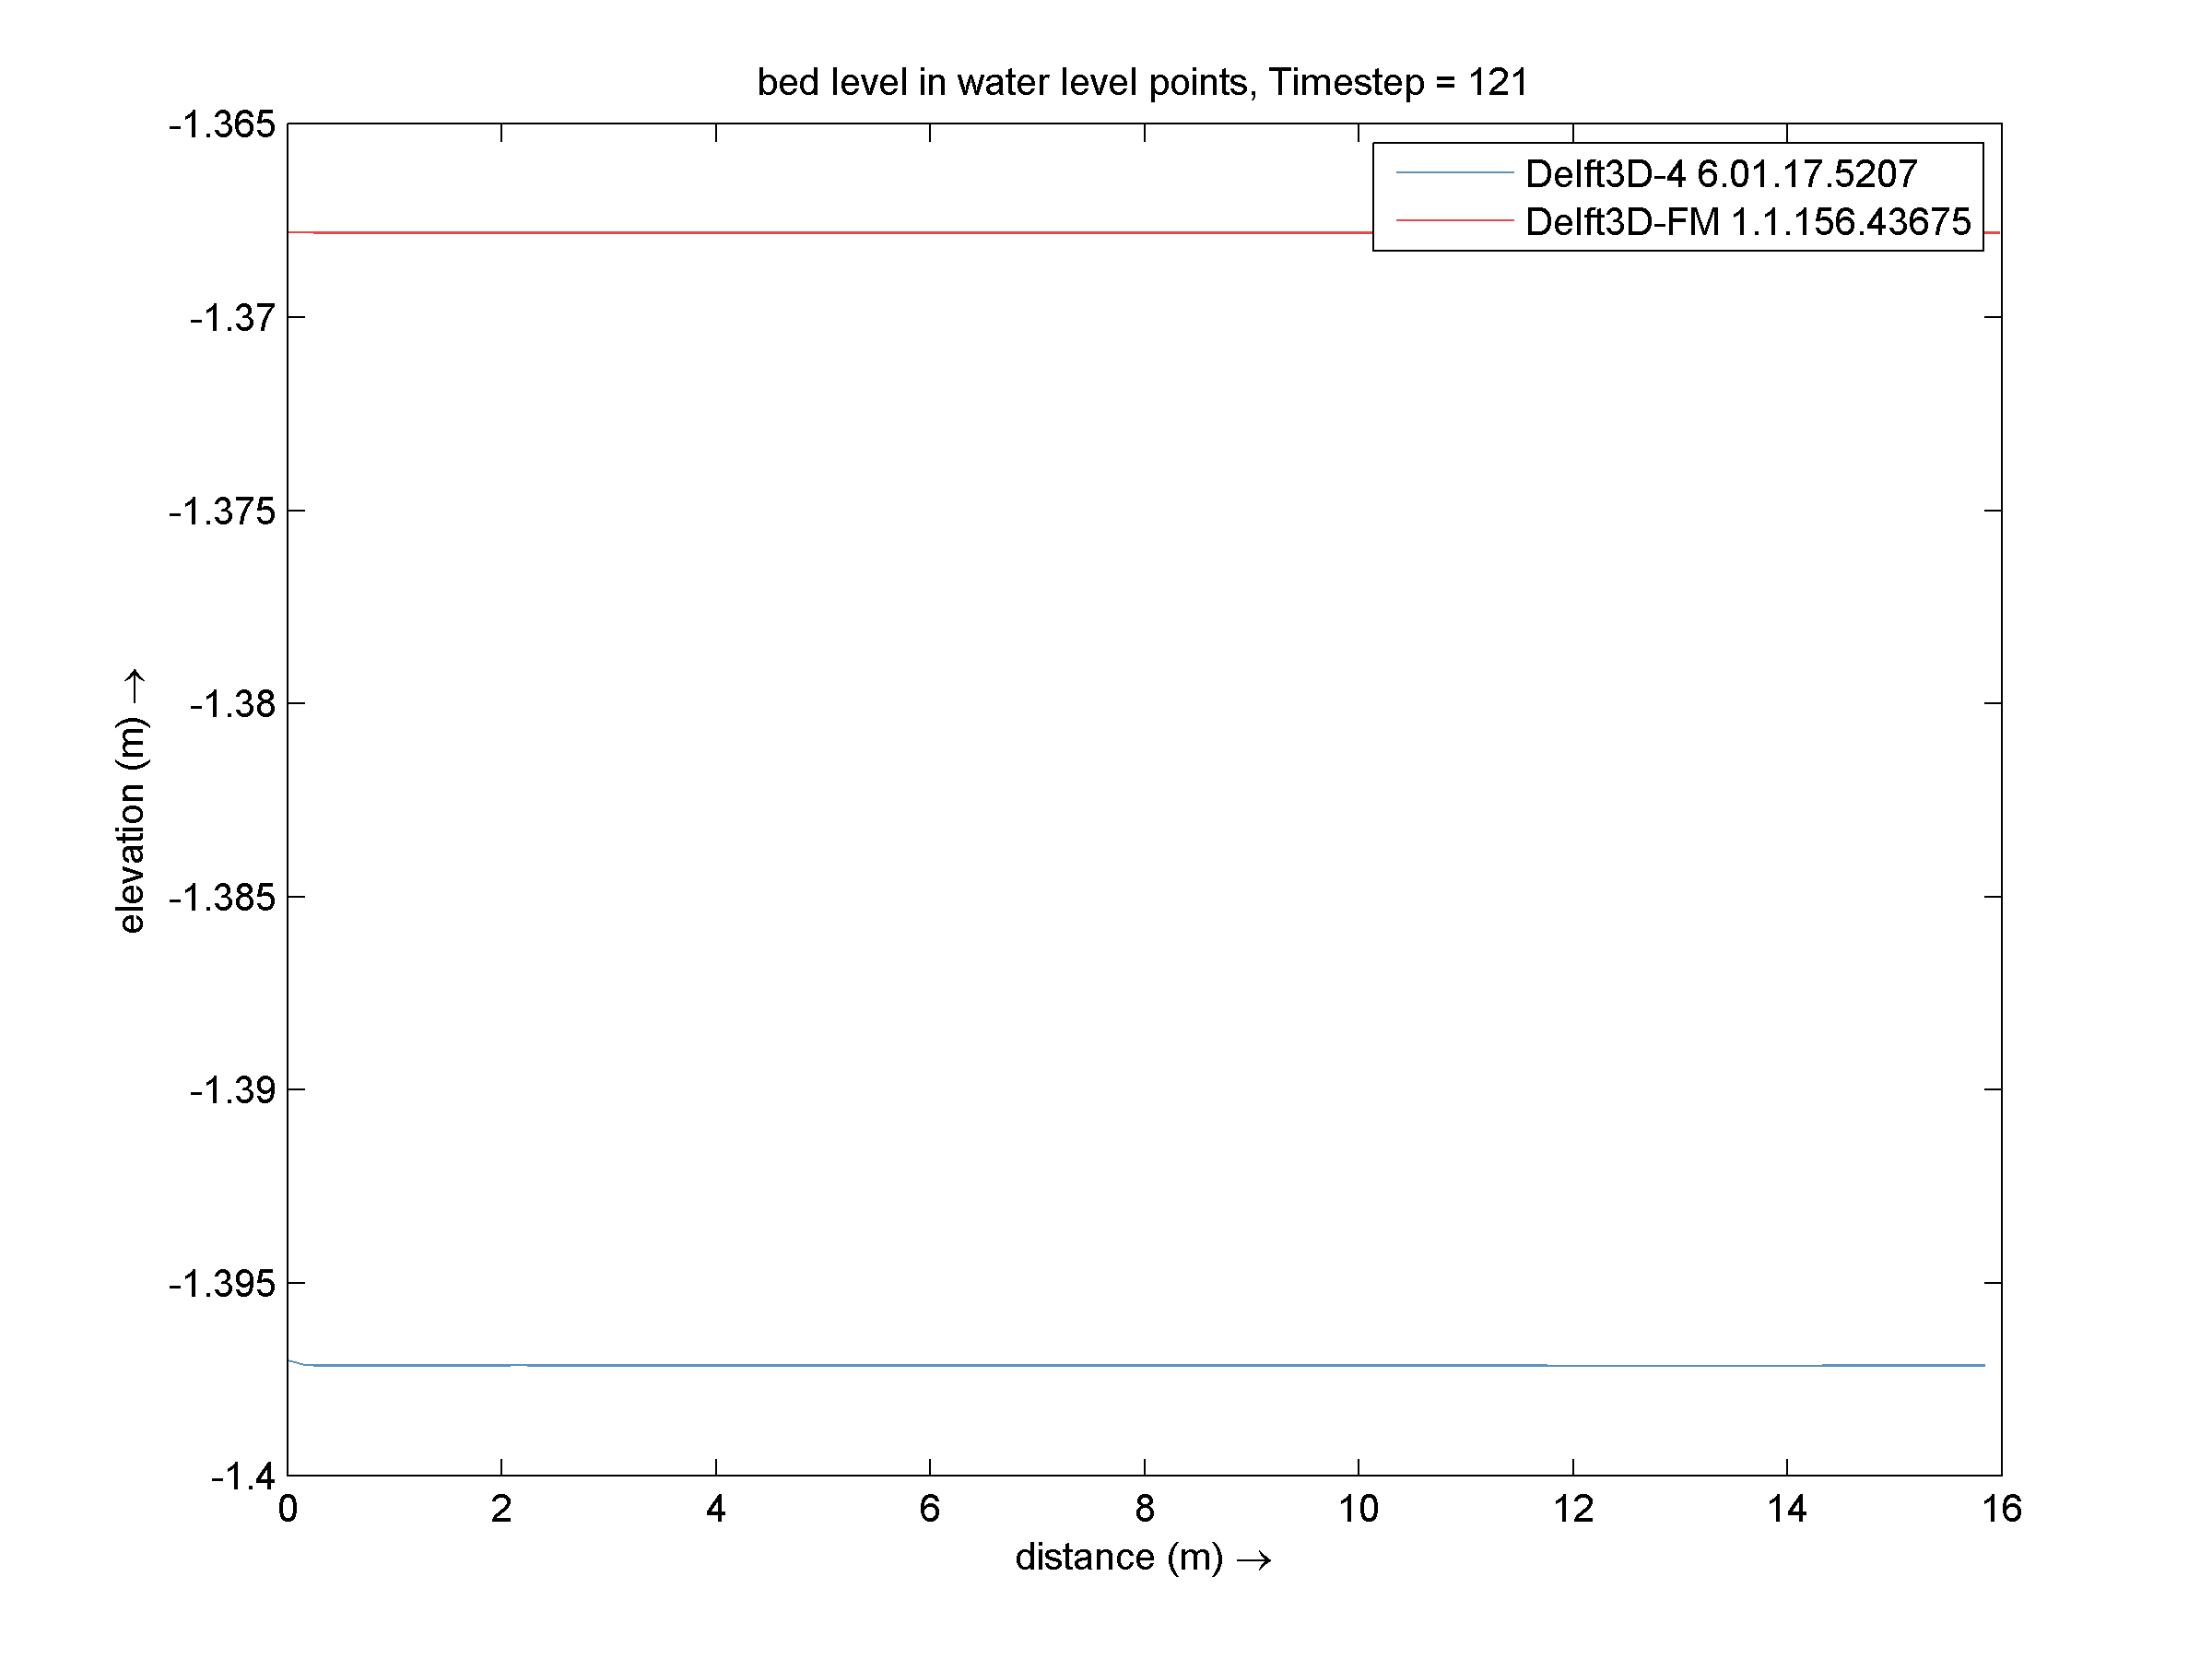
\includegraphics[width=0.70\textwidth]{figures/comparison_d3d_fm_blstr9.png}
	\end{center}
	\caption{Comparison of bed levels (fixed bed boundary condition).}\label{fig:e02-fxx-cxx:bedlevelstr9}
\end{figure}

\begin{figure}[htb]
	\begin{center}
		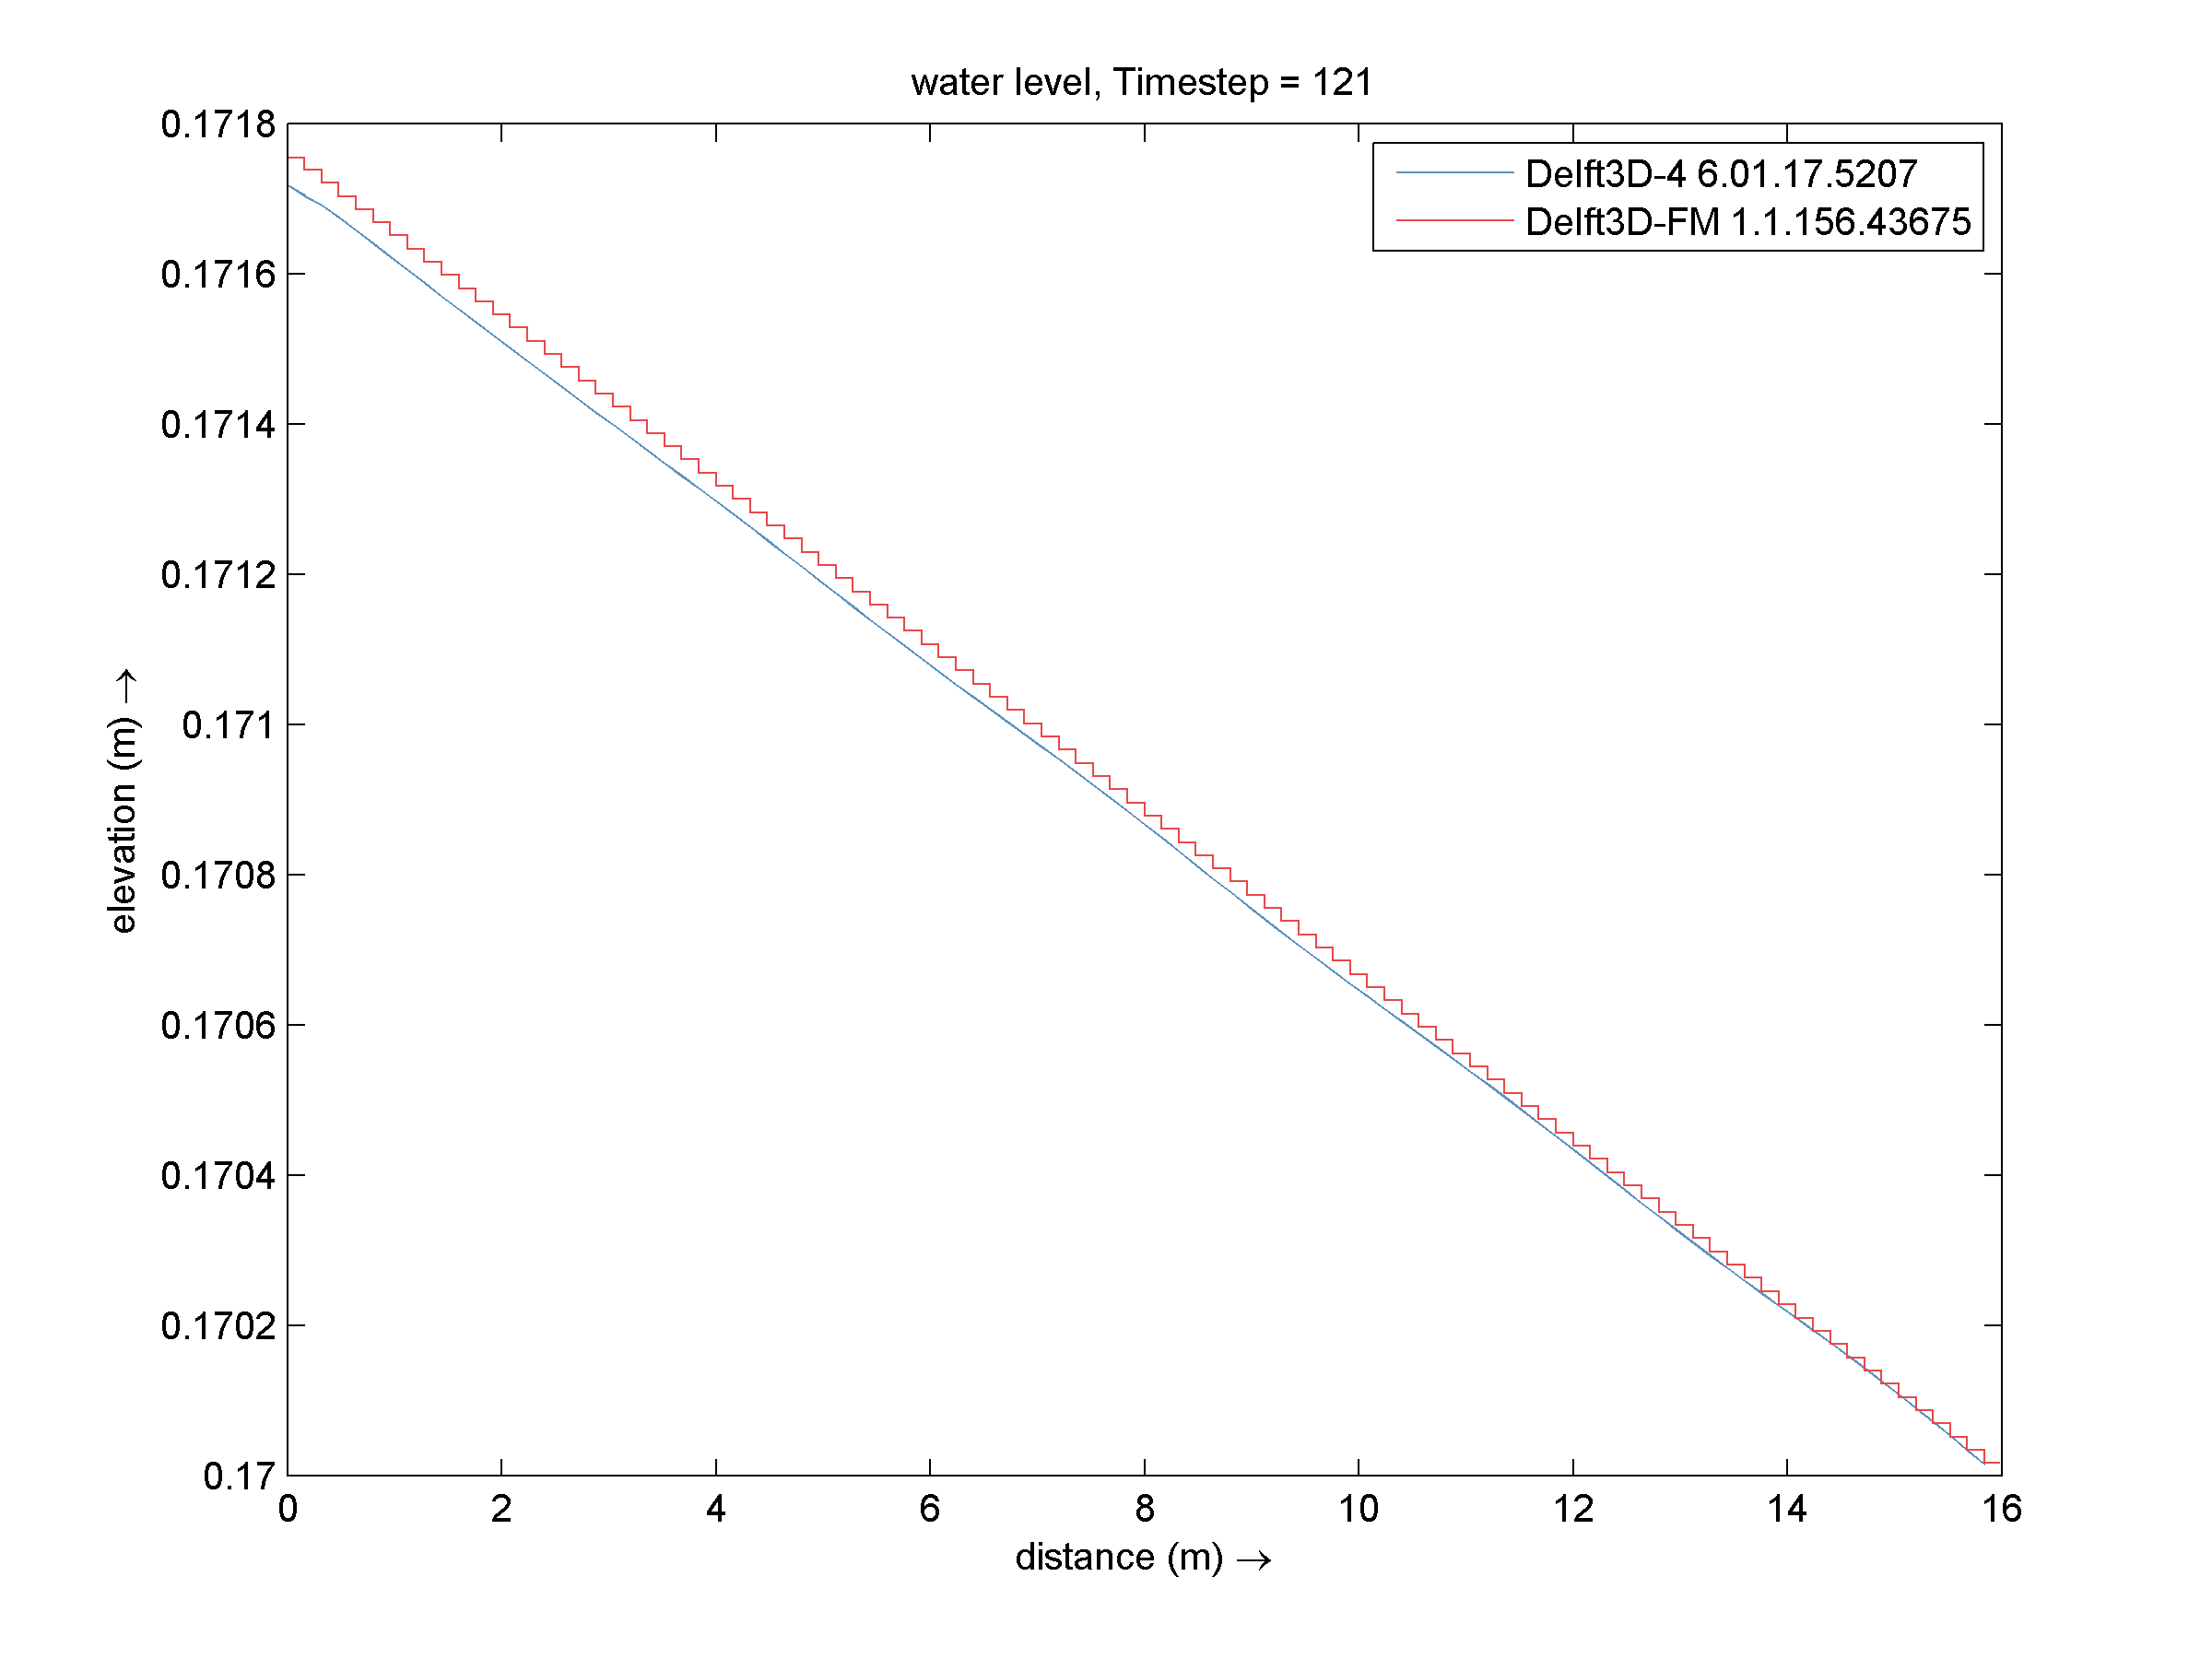
\includegraphics[width=0.70\textwidth]{figures/comparison_d3d_fm_wlstr9.png}
	\end{center}
	\caption{Comparison of water levels (fixed bed boundary condition).}\label{fig:e02-fxx-cxx:waterlevelstr9}
\end{figure}

\begin{figure}[htb]
	\begin{center}
		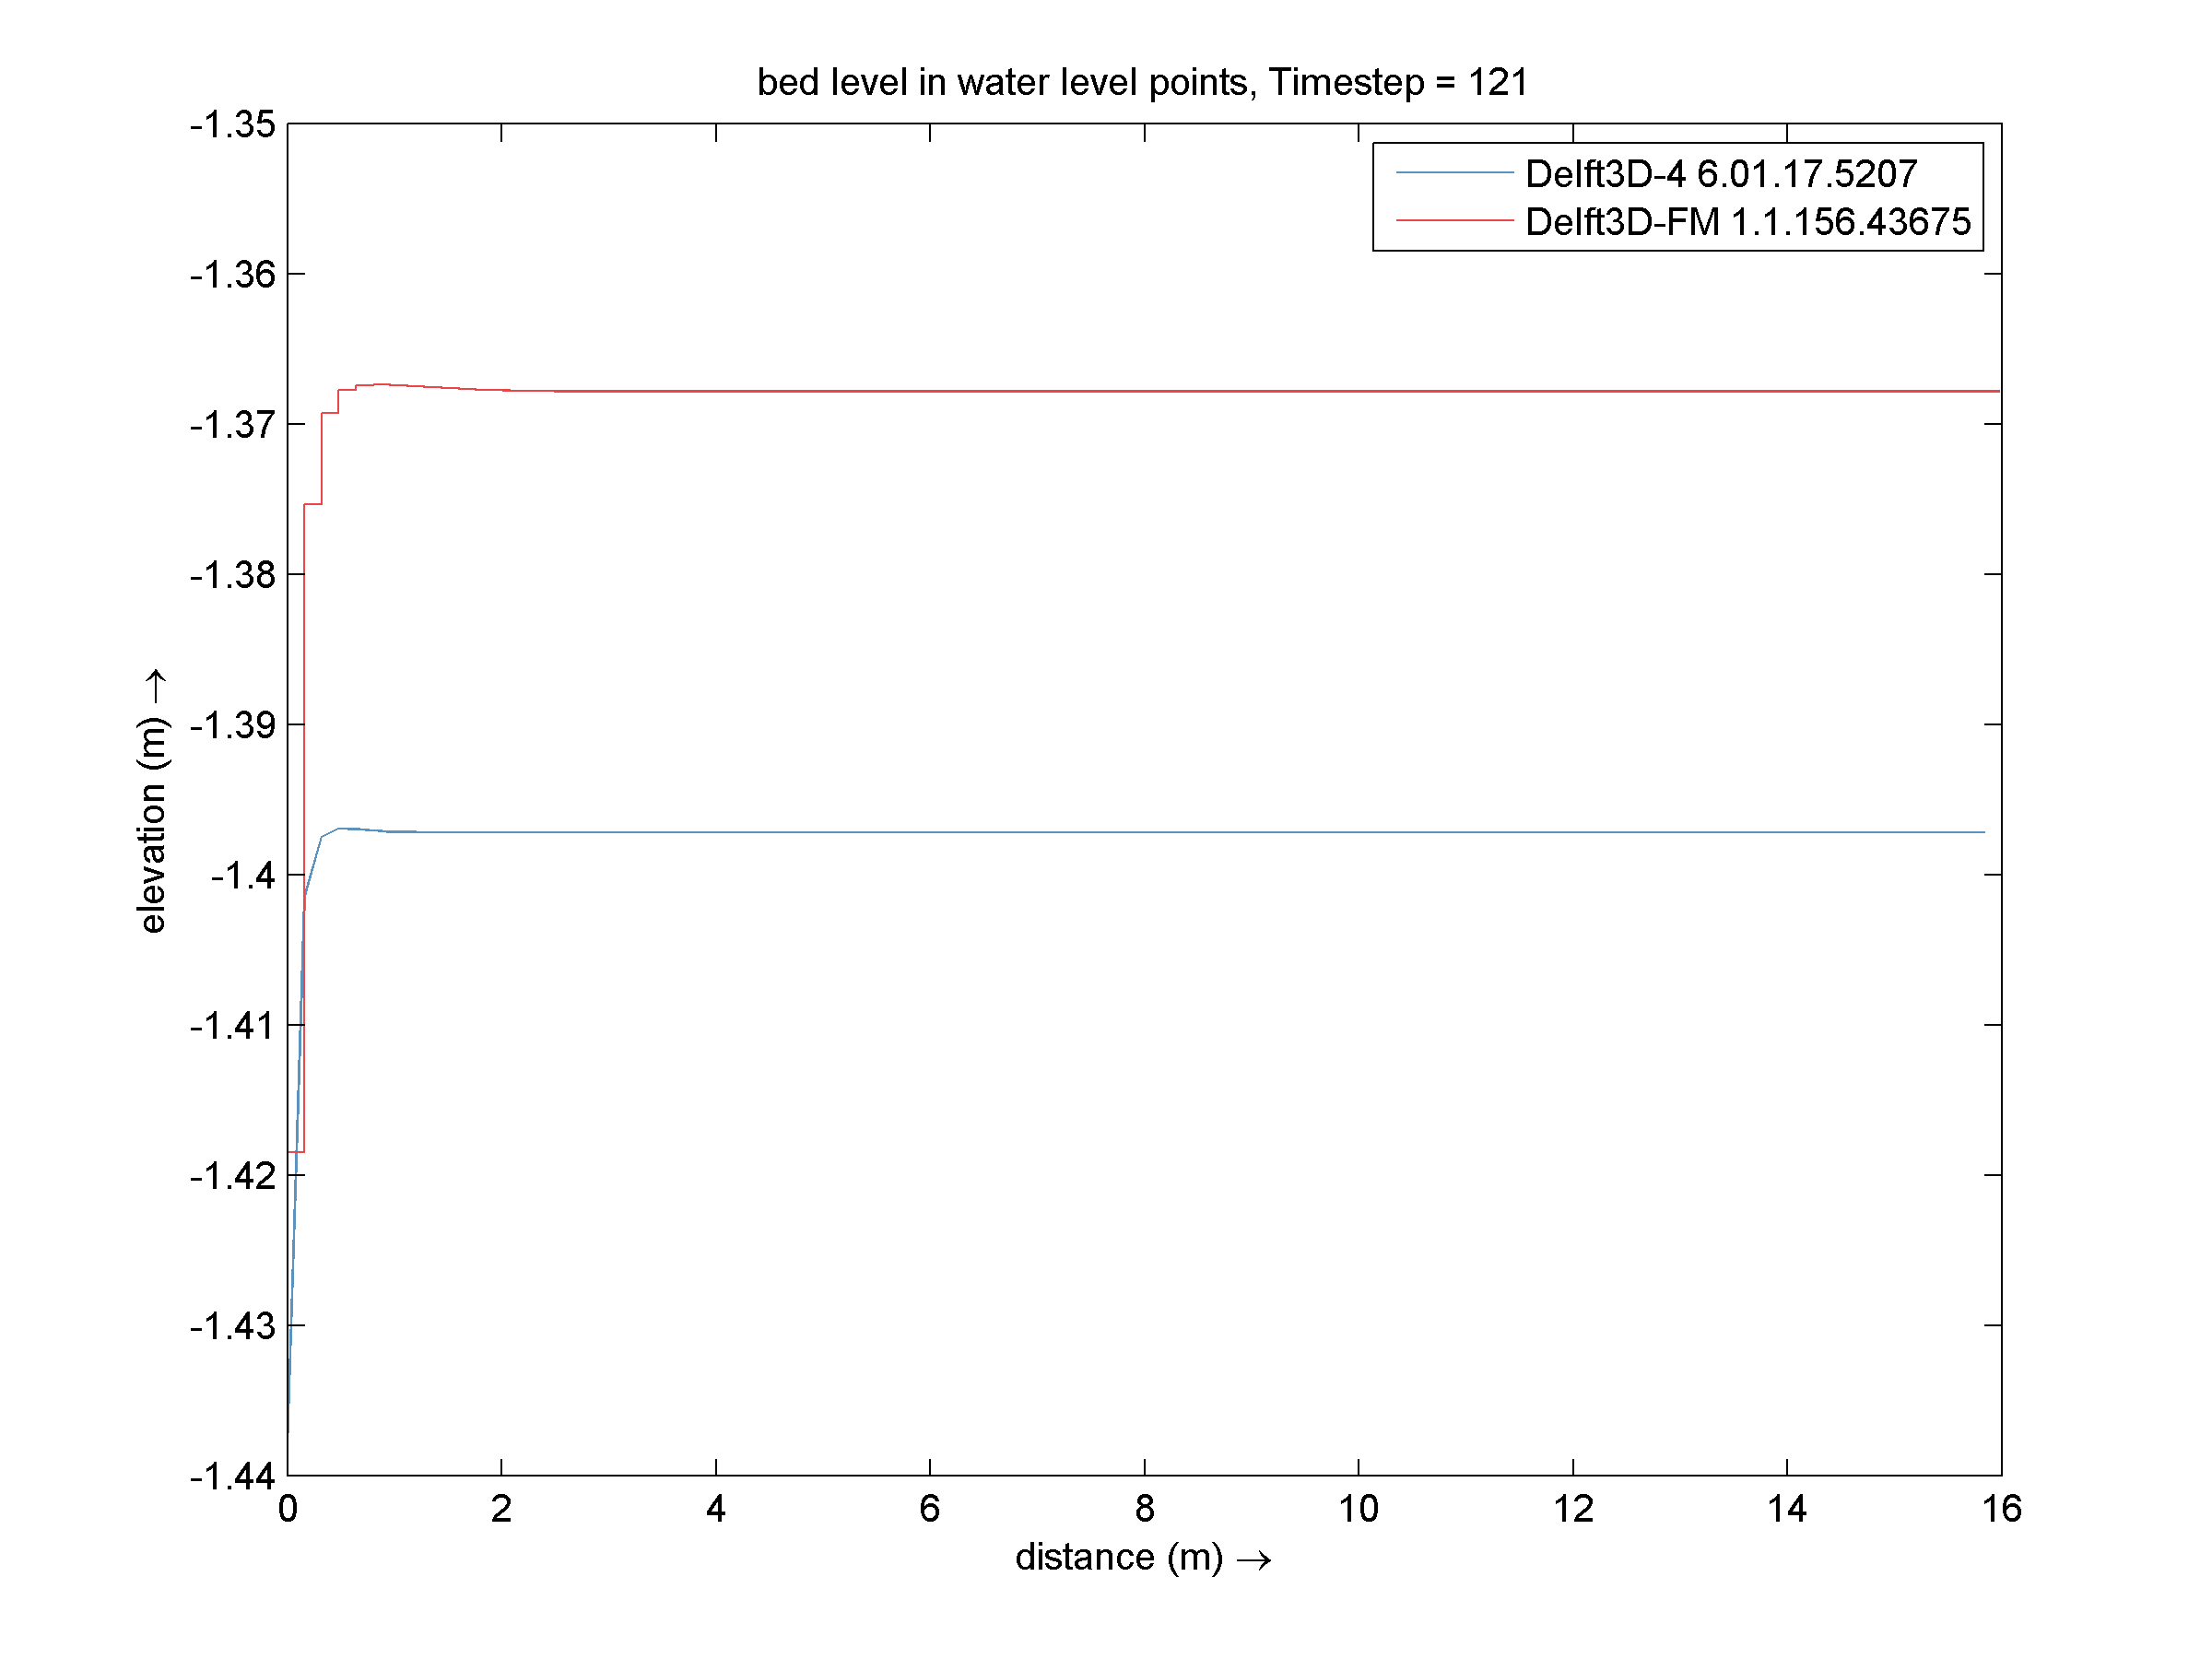
\includegraphics[width=0.70\textwidth]{figures/comparison_d3d_fm_blstr10.png}
	\end{center}
	\caption{Comparison of bed levels ('depth' changes from -1.4 to -1.8 m in 20 min of simulation time).}\label{fig:e02-fxx-cxx:bedlevelstr10}
\end{figure}

\begin{figure}[htb]
	\begin{center}
		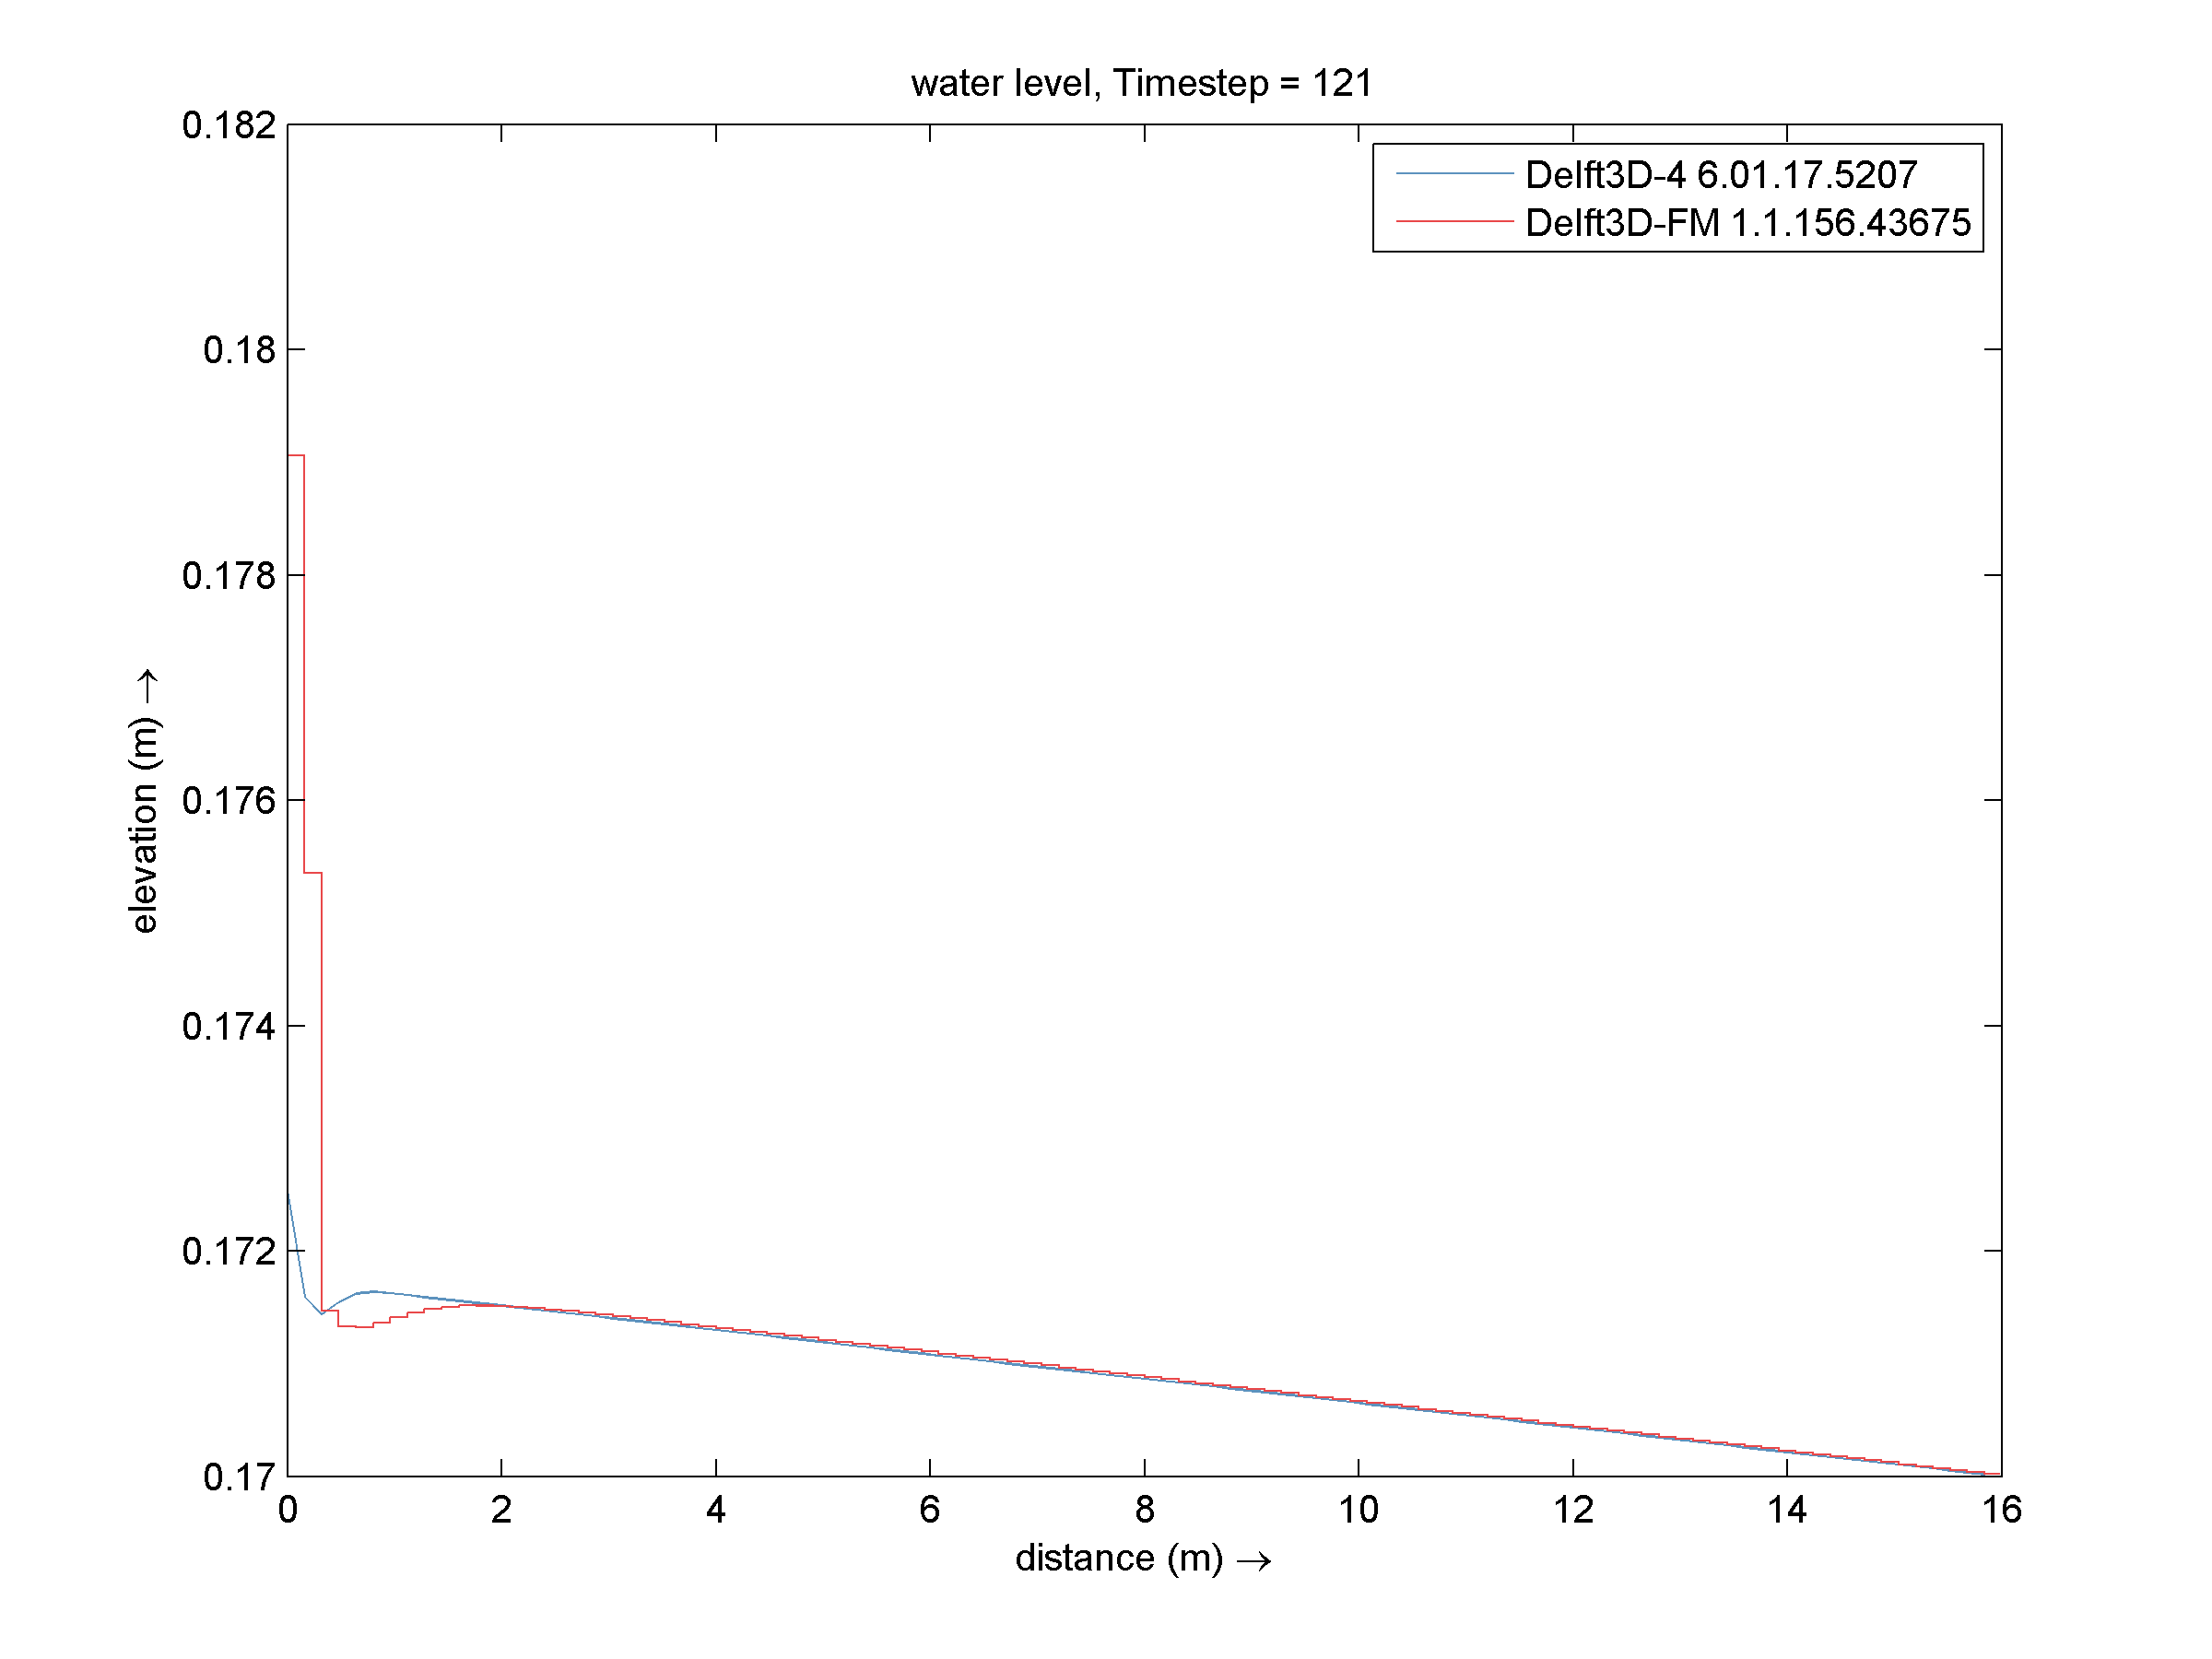
\includegraphics[width=0.70\textwidth]{figures/comparison_d3d_fm_wlstr10.png}
	\end{center}
	\caption{Comparison of water levels ('depth' changes from -1.4 to -1.8 m in 20 min of simuation time).}\label{fig:e02-fxx-cxx:waterlevelstr10}
\end{figure}

\begin{figure}[htb]
	\begin{center}
		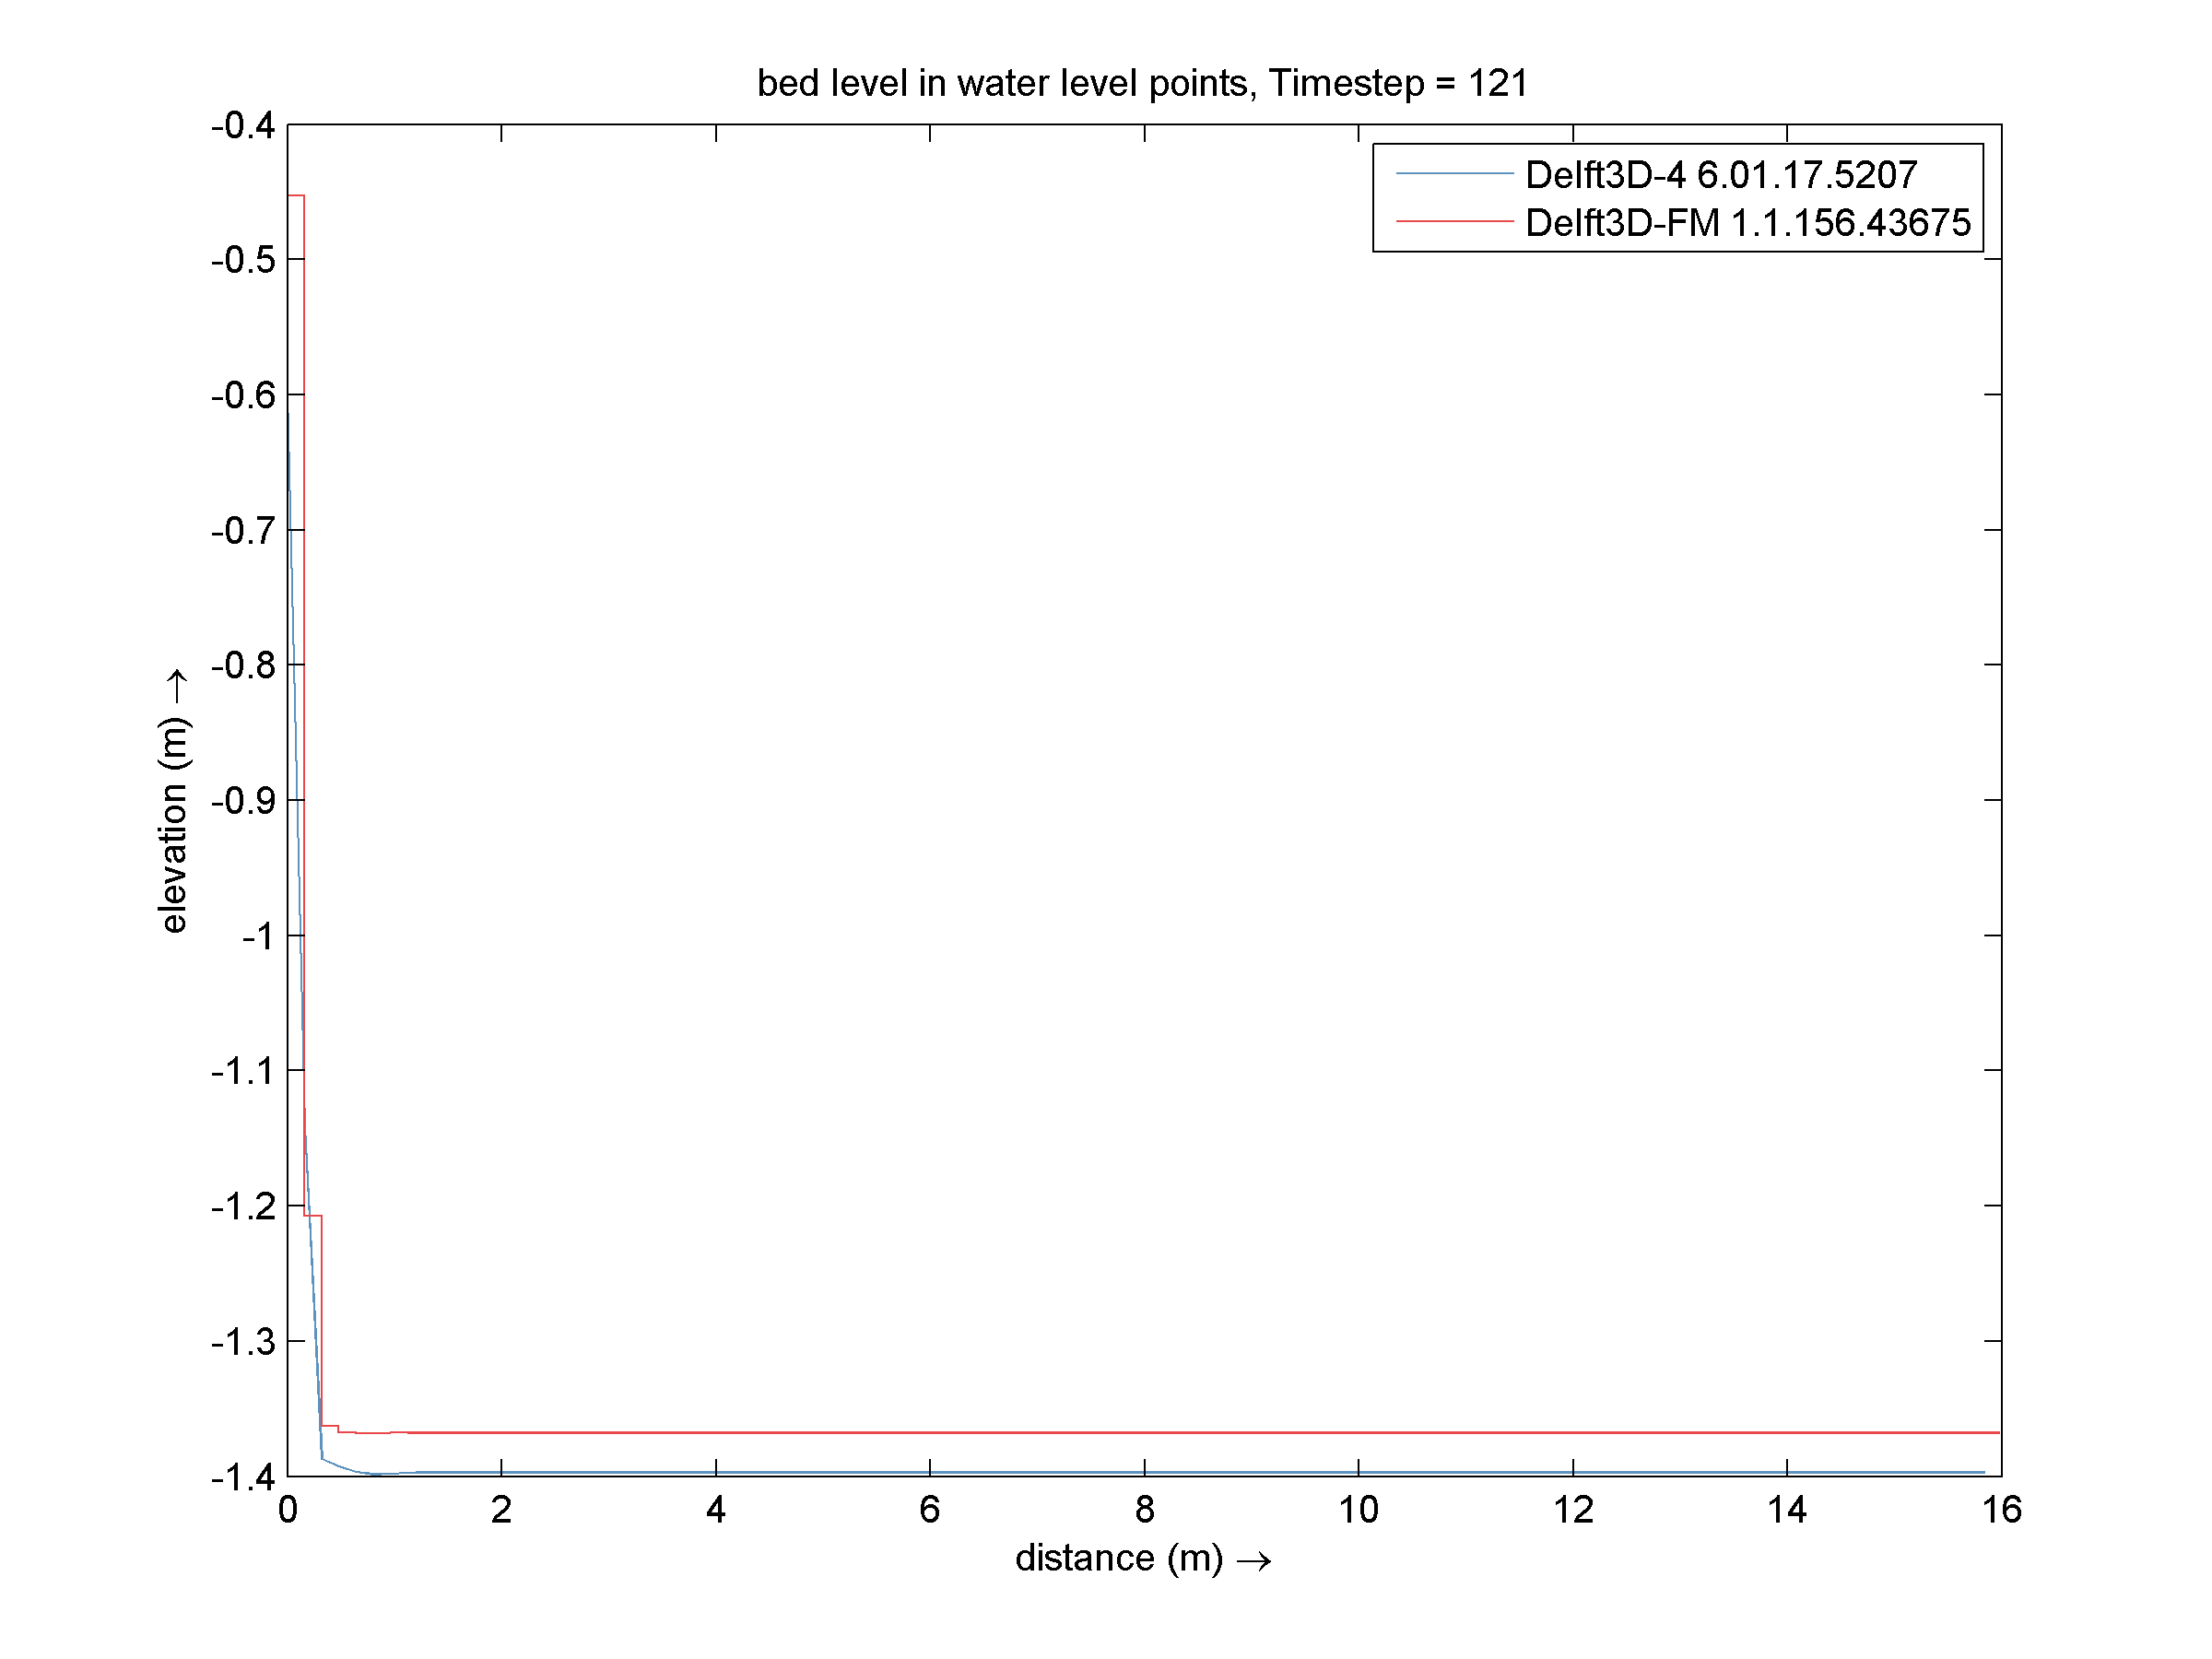
\includegraphics[width=0.70\textwidth]{figures/comparison_d3d_fm_blstr11.png}
	\end{center}
	\caption{Comparison of bed levels ('transport including pores' = 0.0002 m$^2$/s).}\label{fig:e02-fxx-cxx:bedlevelstr11}
\end{figure}

\begin{figure}[htb]
	\begin{center}
		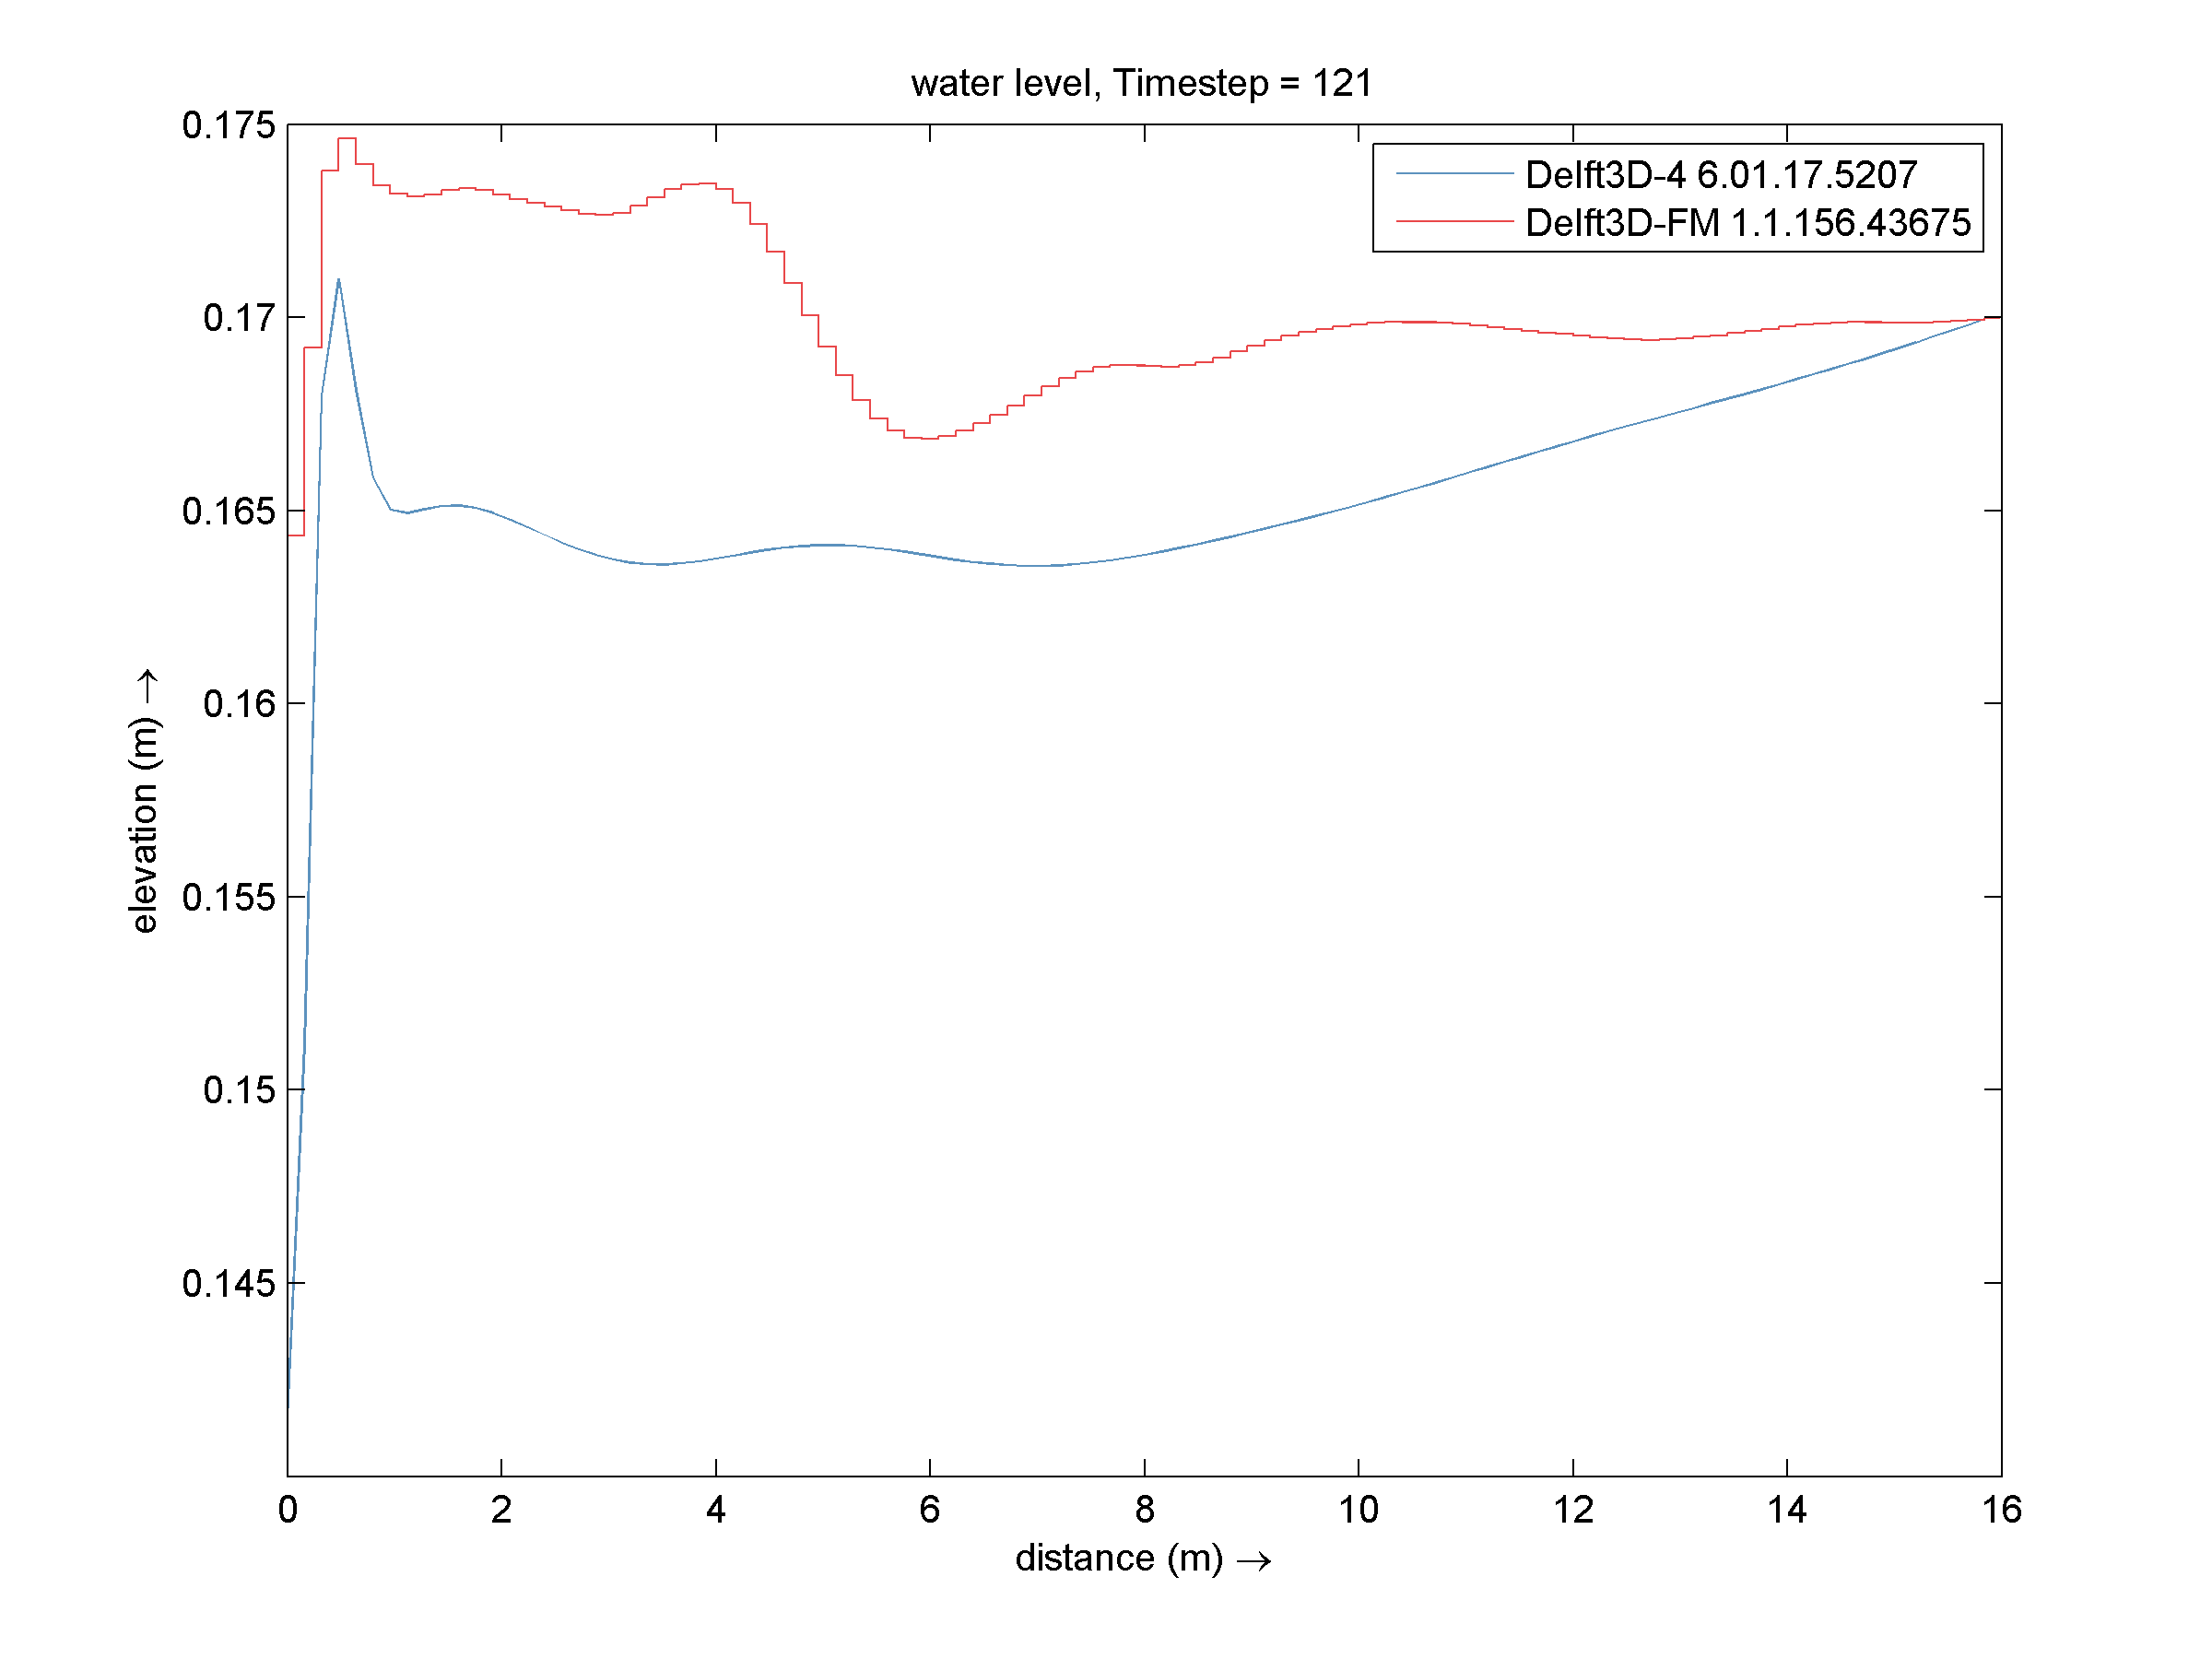
\includegraphics[width=0.70\textwidth]{figures/comparison_d3d_fm_wlstr11.png}
	\end{center}
	\caption{Comparison of water levels ('transport including pores' = 0.0002 m$^2$/s).}\label{fig:e02-fxx-cxx:waterlevelstr11}
\end{figure}

\begin{figure}[htb]
	\begin{center}
		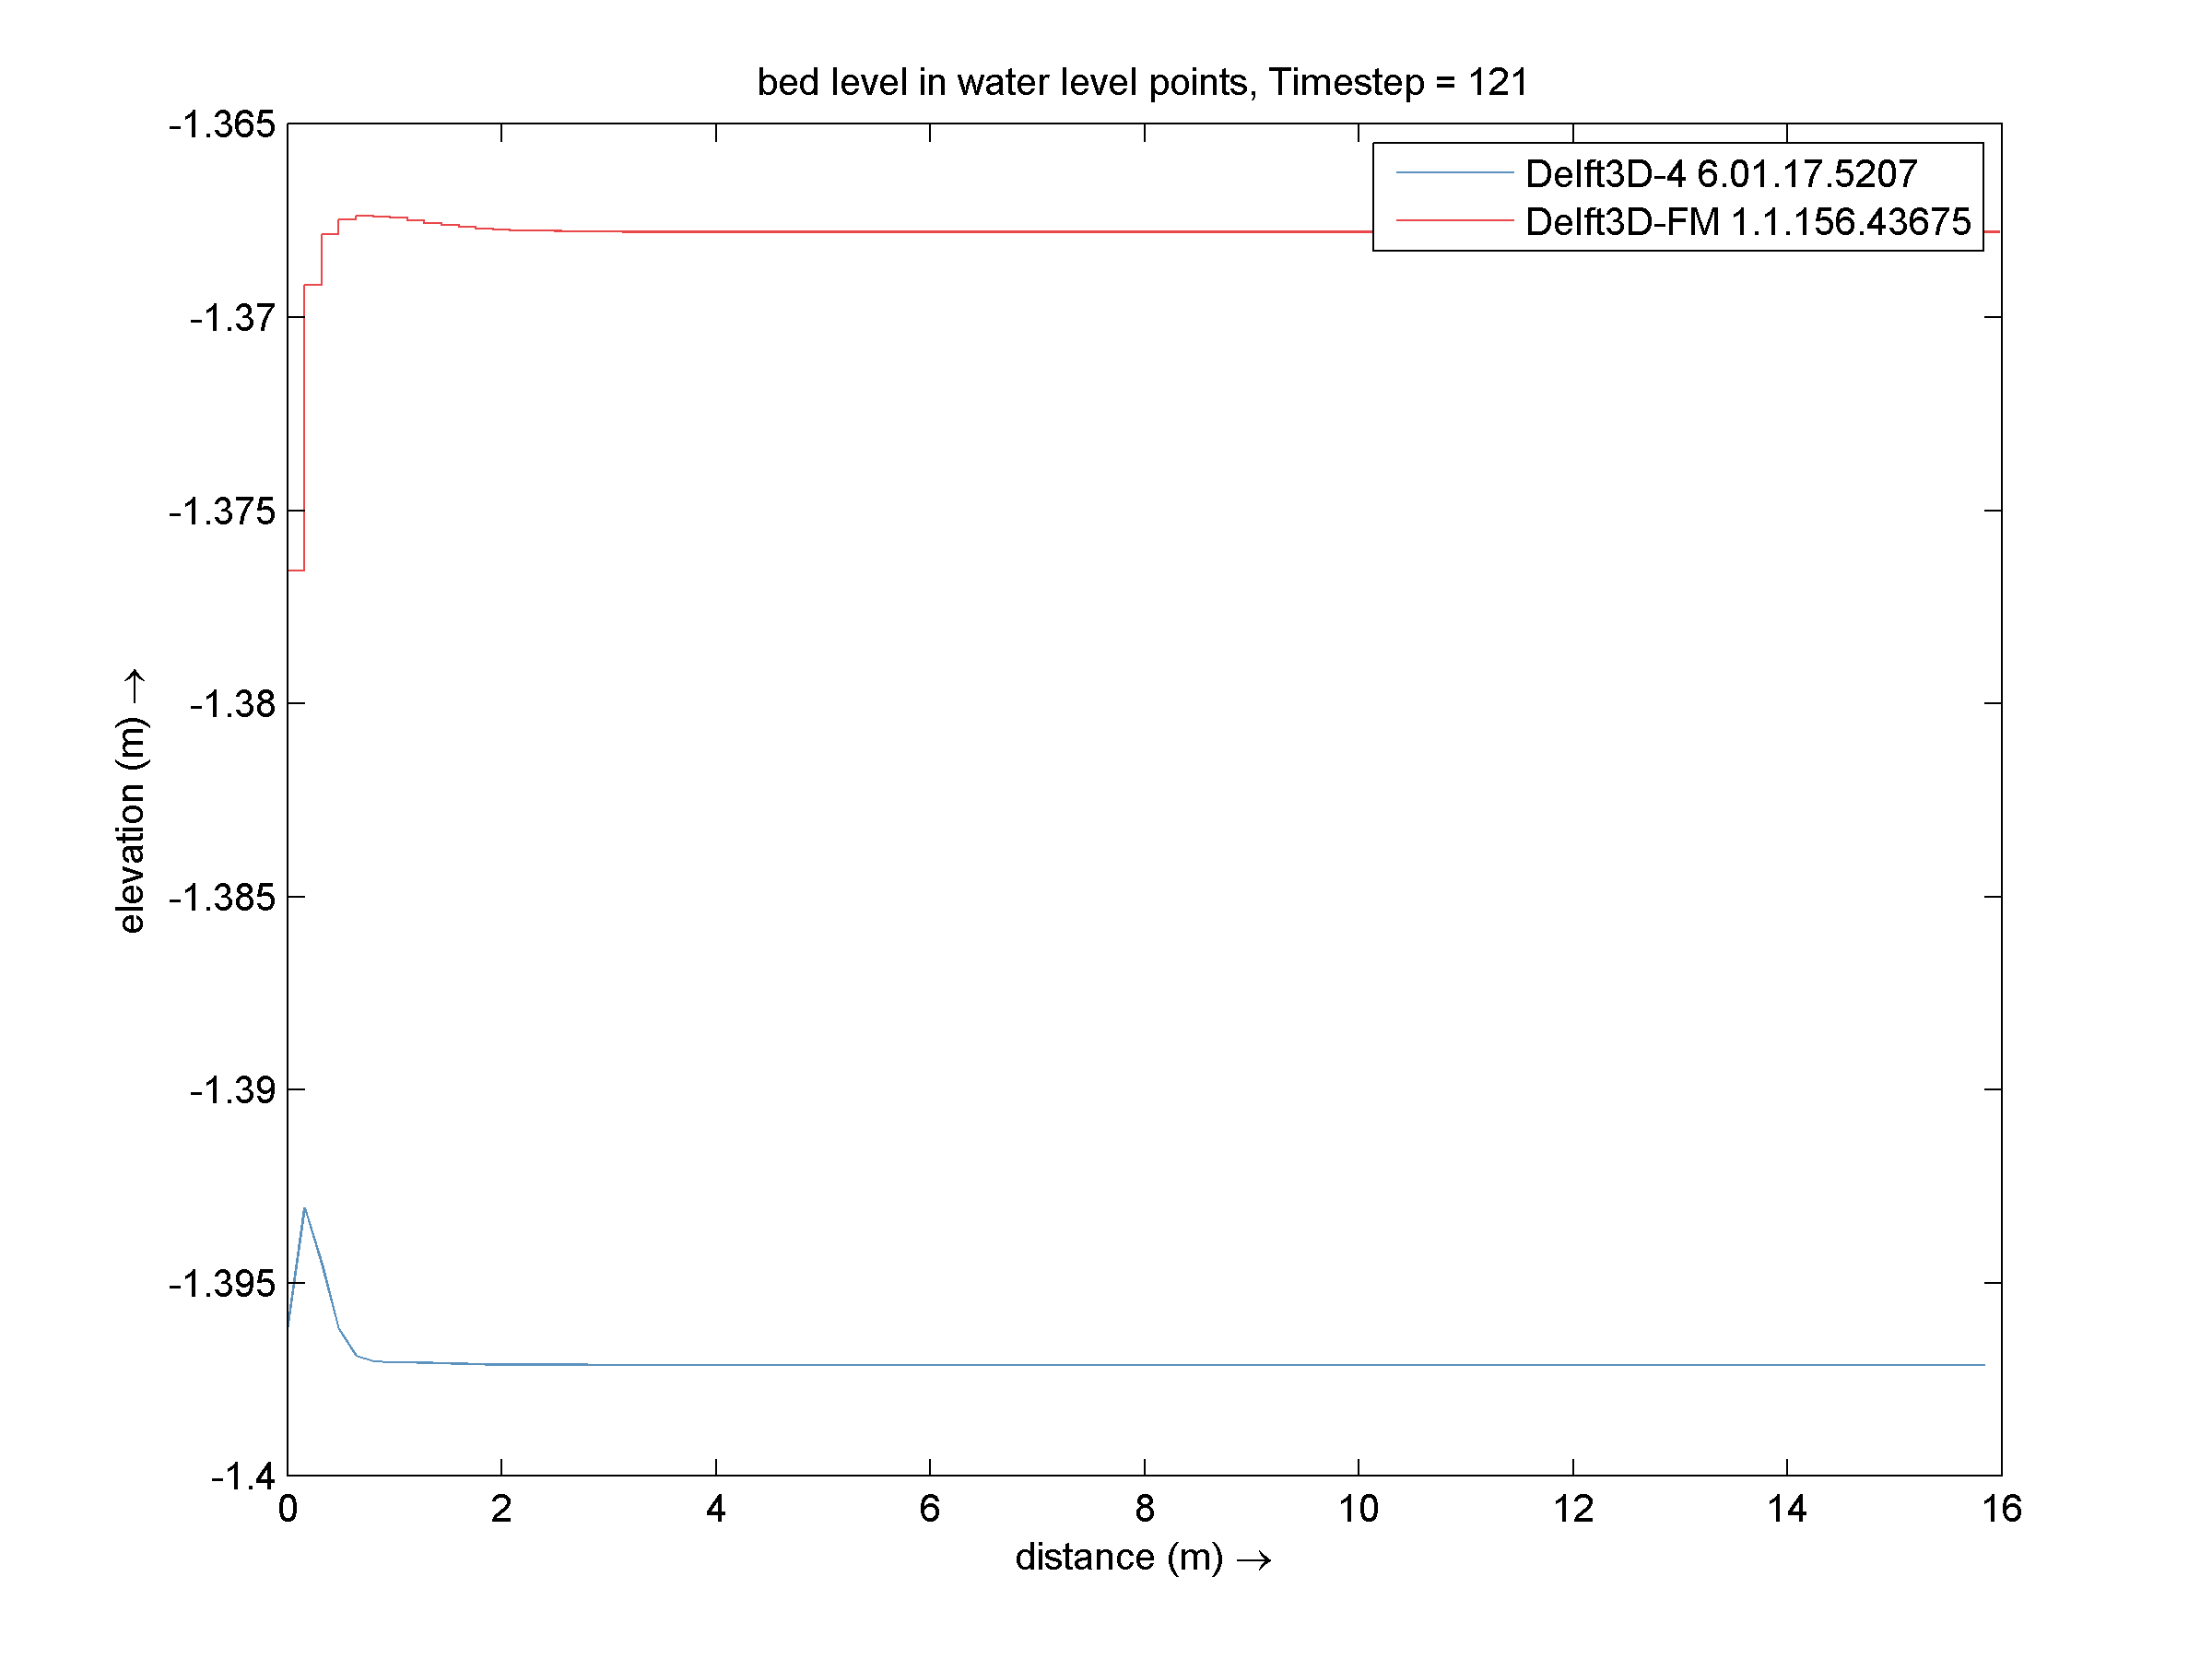
\includegraphics[width=0.70\textwidth]{figures/comparison_d3d_fm_blstr12.png}
	\end{center}
	\caption{Comparison of bed levels ('depth' = -1.4 m).}\label{fig:e02-fxx-cxx:bedlevelstr12}
\end{figure}

\begin{figure}[htb]
	\begin{center}
		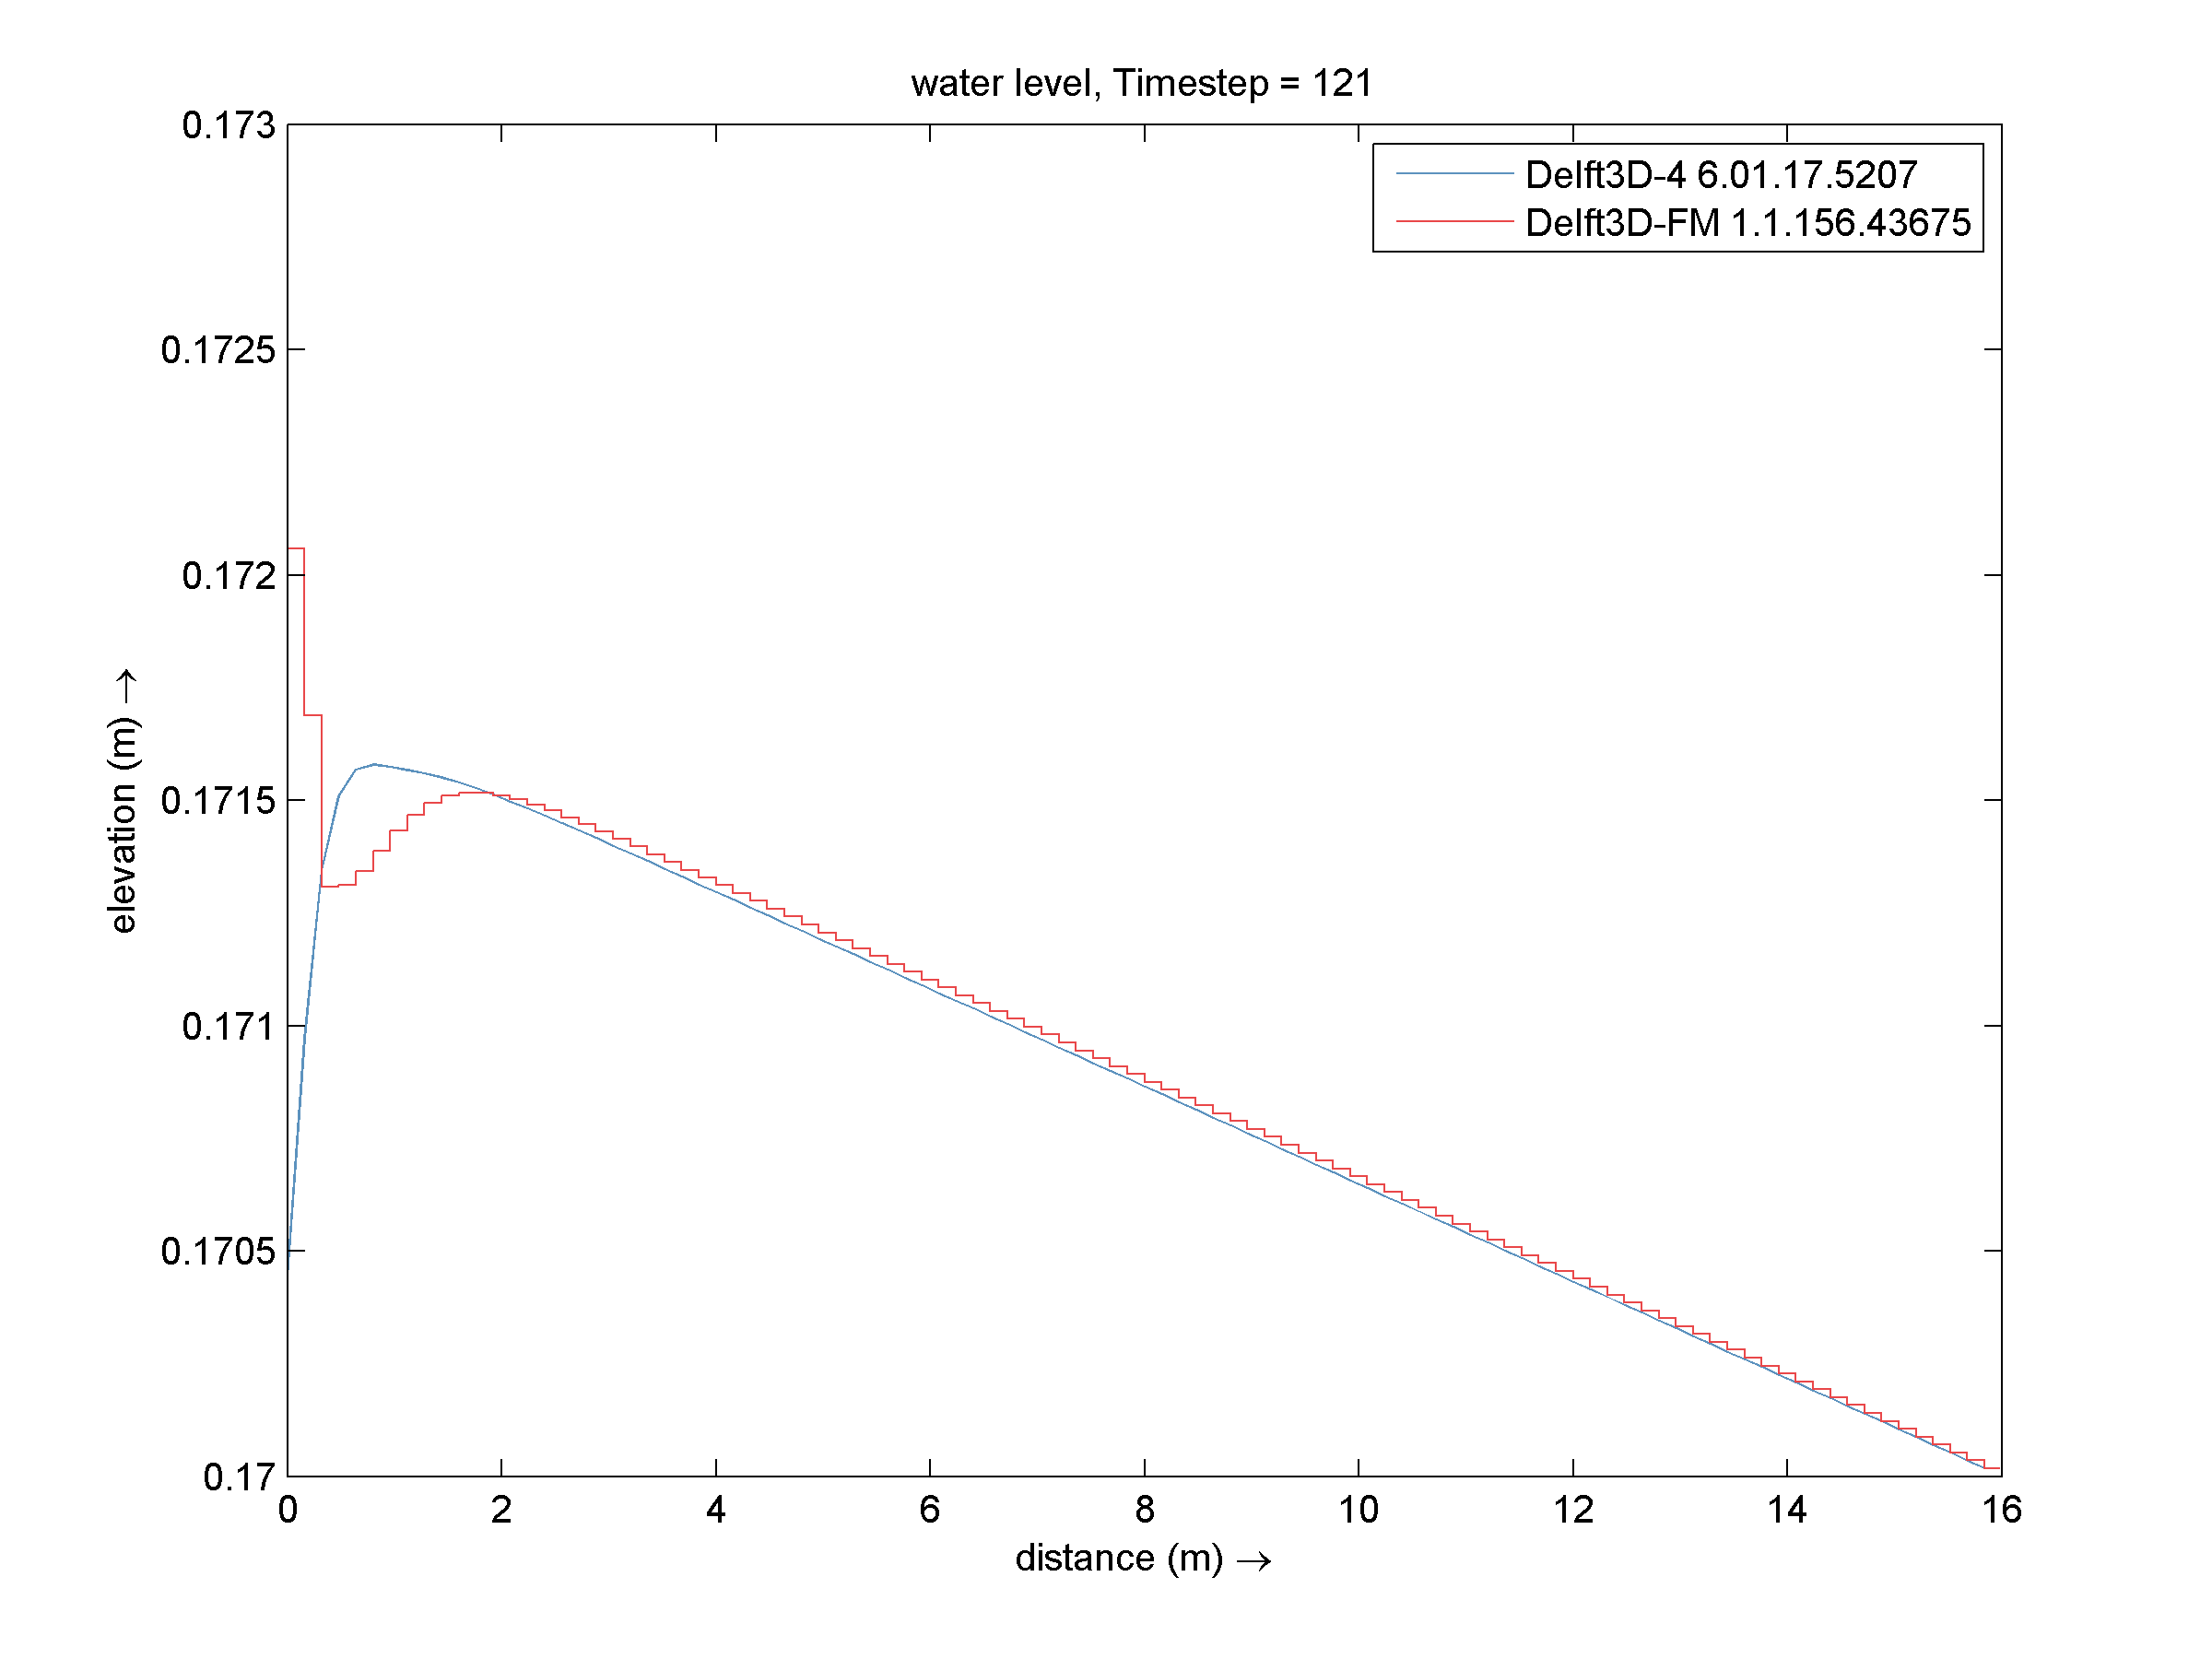
\includegraphics[width=0.70\textwidth]{figures/comparison_d3d_fm_wlstr12.png}
	\end{center}
	\caption{Comparison of water levels ('depth' = -1.4 m).}\label{fig:e02-fxx-cxx:waterlevelstr12}
\end{figure}


